\documentclass[letterpaper,12pt]{book}

\usepackage{amsmath, amsfonts, amscd, amssymb, amsthm}
%\usepackage{import}
\usepackage{versions}
\usepackage{crop}
\usepackage{multicol}
\usepackage{graphicx}
\usepackage{listings}
\lstset{basicstyle=\footnotesize\ttfamily, language=Python}
\usepackage{makeidx}
\usepackage[pageanchor=false]{hyperref}
\usepackage{ifthen}
\usepackage[format=hang,font=normalsize,labelfont=bf]{caption}
\usepackage{subcaption}
\usepackage{natbib}
\usepackage{chapterbib}
\usepackage[nottoc]{tocbibind}
\usepackage{setspace}
\usepackage{placeins}
\usepackage{framed}
\usepackage{enumitem}
\usepackage{threeparttable}
\usepackage{geometry}
\geometry{letterpaper,tmargin=1in,bmargin=1in,lmargin=1in,rmargin=1in}
\usepackage{multirow}
\usepackage{array}
\usepackage{delarray}
\usepackage{lscape}
\usepackage{float,color, colortbl}
%\usepackage[pdftex]{graphicx}
\usepackage{hyperref}
\usepackage{tabu}
\usepackage{appendix}
\usepackage{verbatim}


\usepackage{bm}
\usepackage{color}

\lstset{frame=single,
  language=Python,
  showstringspaces=false,
  columns=flexible,
  basicstyle={\small\ttfamily},
  numbers=none,
  breaklines=true,
  breakatwhitespace=true
  tabsize=3
}


\include{thmstyle}
\bibliographystyle{aer}
\providecommand{\abs}[1]{\lvert#1\rvert}
\newcommand\norm[1]{\left\lVert#1\right\rVert}
\newcommand{\ve}{\varepsilon}
\newcommand{\ip}[2]{\langle #1,#2 \rangle}

\hypersetup{colorlinks,linkcolor=red,urlcolor=blue,citecolor=red}
\theoremstyle{definition}
\newtheorem{theorem}{Theorem}[chapter] % Number theorems by chapter
\newtheorem{acknowledgement}[theorem]{Acknowledgement}
\newtheorem{algorithm}[theorem]{Algorithm}
\newtheorem{axiom}[theorem]{Axiom}
\newtheorem{case}[theorem]{Case}
\newtheorem{claim}[theorem]{Claim}
\newtheorem{conclusion}[theorem]{Conclusion}
\newtheorem{condition}[theorem]{Condition}
\newtheorem{conjecture}[theorem]{Conjecture}
\newtheorem{corollary}[theorem]{Corollary}
\newtheorem{criterion}[theorem]{Criterion}
\newtheorem{definition}{Definition}[chapter] % Number definitions by chapter
\newtheorem{derivation}{Derivation}[chapter] % Number derivations by chapter
\newtheorem{example}[theorem]{Example}
\newtheorem{exercise}{Exercise}[chapter] % Number exercises by chapter
\newtheorem{lemma}[theorem]{Lemma}
\newtheorem{notation}[theorem]{Notation}
\newtheorem{problem}[theorem]{Problem}
\newtheorem{proposition}{Proposition}[chapter] % Number propositions by chapter
\newtheorem{remark}[theorem]{Remark}
\newtheorem{solution}[theorem]{Solution}
\newtheorem{summary}[theorem]{Summary}
\numberwithin{equation}{chapter}
\renewcommand\theenumi{\roman{enumi}}
\DeclareMathOperator*{\argmin}{arg\,min}
\DeclareMathOperator*{\argmax}{arg\,max}
\newcommand{\ogusa}{\texttt{OG-USA}\,}
\newcommand{\ogindia}{\texttt{OG-India}\,}
\newcommand{\git}{\texttt{Git}\,}
\newcommand{\taxcalc}{\texttt{Tax-Calculator}\,}
\newcommand{\btax}{\texttt{B-Tax}\,}


%\numberwithin{Exercise}{chapter}

\sectionbib{\section*}{section}

\crop
\makeindex

\begin{document}

\frontmatter

\title{OG-India: Documentation for the Large-scale Dynamic General Equilibrium Overlapping Generations Model for Indian Policy Analysis}
\author{Richard W. Evans\\ \emph{University of Chicago} \and Jason DeBacker \\ \emph{University of South Carolina}}
\date{\LARGE{August 2019} \\
{\footnotesize{(version 2019.08.b)}}}
\maketitle

\chapter{Preface}

  The development of this model benefited from support from the Tax Policy Research Unit of India as well as from the Open Source Economics Laboratory at the University of Chicago an Open Research Group, Inc. All Python code for the computational model is available at \href{https://github.com/TPRU-India/OG-India}{https://github.com/TPRU-India/OG-India}. Contributions to the model code can also be viewed in detail on the OG-India \href{https://github.com/TPRU-India/OG-India/graphs/contributors}{contributions page}.

\setcounter{tocdepth}{1}
\tableofcontents


\mainmatter

\part{Introduction}
  \chapter{Introduction}\label{Chap_Intro}
    %!TEX root = ../OGUSAdoc.tex

The overlapping generations model is a workhorse of dynamic fiscal analysis. \ogindia is dynamic in that households in the model make consumption, savings, and labor supply decisions based on their expectations over their entire lifetime, not just the current period. Because \ogindia is a general equilibrium model, behavioral changes by households and firms can cause macroeconomic variables and prices to adjust.

But the main characteristic that differentiates the overlapping generations model from other dynamic general equilibrium models is its realistic modeling of the finite lifetimes of individuals and the cross-sectional age heterogeneity that exists in the economy. One can make a strong case that age heterogeneity and income heterogeneity are two of the main sources of diversity that explain much of the behavior in which we are interested for policy analysis.

\ogindia can be summarized as having the following characteristics.
\begin{itemize}
  \item Households
  \begin{itemize}
    \item overlapping generations of finitely lived households
    \item households are forward looking and see to maximize their expected lifetime utility, which is a function of consumption, labor supply, and bequests
    \item households choose consumption, savings, and labor supply every period.
    \item The only uncertainty households face is with respect to their mortality risk
    \item realistic demographics: mortality rates, fertility rates, immigration rates, population growth, and population distribution dynamics
    \item heterogeneous lifetime income groups within each age cohort, calibrated from U.S. tax data
    \item incorporation of detailed household tax data from \taxcalc microsimulation model
    \item calibrated intentional and unintentional bequests by households to surviving generations
  \end{itemize}
  \item Firms
  \begin{itemize}
    \item representative perfectly competitive firm maximizes static profits with general CES production function by choosing capital and labor demand
    \item exogenous productivity growth is labor augmenting technological change
    \item firms face a corporate income tax as well as various depreciation deductions and tax treatments
  \end{itemize}
  \item Government
  \begin{itemize}
    \item government collects tax revenue from households and firms
    \item government distributes transfers to households
    \item government spends resources on public goods
    \item government can run deficits and surpluses
    \item a stabilization rule (budget closure rule) must be implemented at some point in the time path if government debt is growing at a rate permanently different from GDP.
  \end{itemize}
  \item Aggregate, market clearing, and international
  \begin{itemize}
    \item Aggregate model is deterministic (no aggregate shocks)
    \item Three markets must clear: capital, labor, and goods markets
    \item
  \end{itemize}
\end{itemize}

%%% Put summary of the general incentives in the model, overall implications of the assumptions, and particularly how these interact with tax policy

We will update this document as more detail is added to the model.

  \chapter{Exogenous Inputs and Endogenous Output}\label{Chap_ExogEndog}
    %!TEX root = ../OGUSAdoc.tex

In this chapter, list the exogenous inputs to the model, options, and where the values come from (weak calibration vs. strong calibration). Point to the respective chapters for some of the inputs. Mention the code \texttt{parameters.py}.

Also go through the output of the model, endogenous variables, and potential tables and pictures to produce.


\section{Exogenous Parameters}\label{SecExEnd_Exog}

  List all the exogenous parameters that are outputs of the model here.

  \begin{table}[htbp] \centering \captionsetup{width=4.7in}
    \caption{\label{TabExogVars}\textbf{List of exogenous parameters and baseline calibration values}}
      \begin{threeparttable}
      \begin{tabular}{>{\footnotesize}c |>{\footnotesize}l |>{\footnotesize}c}
        \hline\hline
        Symbol & \multicolumn{1}{c}{\footnotesize{Description}} & Value \\
        \hline
        $S$ & Maximum periods in economically active & 80 \\[-1.5mm]
        & \quad household life & \\
        $E$ & Number of periods of youth economically & $\text{round}\left(\frac{S}{4}\right)=20$ \\[-1.5mm]
        & \quad outside the model & \\
        $R$ & Retirement age (period) & $E+\text{round}\left(\frac{9}{16}S\right)=65$ \\
        $T_1$ & Number of periods to steady state for initial & 160 \\[-1.5mm]
        & \quad time path guesses & \\
        $T_2$ & Maximum number of periods to steady state & 160 \\[-1.5mm]
        & \quad for nonsteady-state equilibrium & \\
        $\nu$ & Dampening parameter for TPI & 0.4 \\
        \hline
        $\{\{\omega_{s,0}\}_{s=1}^{E+S}\}_{t=0}^{T_2+S-1}$ & Initial population distribution by age & (see Ch. \ref{Chap_Demog}) \\
        $\{f_s\}_{s=1}^{E+S}$ & Fertility rates by age & (see Sec. \ref{SecDemogFert}) \\
        $\{i_s\}_{s=1}^{E+S}$ & Immigration rates by age & (see Sec. \ref{SecDemogMort}) \\
        $\{\rho_s\}_{s=0}^{E+S}$ & Mortality rates by age & (see Sec. \ref{SecDemogImm}) \\

        % $\bm{\hat{\Gamma}}_1$ & Initial distribution of savings & $\bm{\bar{\Gamma}}$ \\

        % $\{e_{j,s}\}_{j,s=1}^{J,S}$ & Deterministic ability process & (see \citealp{DEMPRW2015}) \\
        % $\{\lambda_j\}_{j=1}^J$ & Lifetime income group percentages & $[0.25,0.25,0.20,0.10,0.10,0.09,0.01]$ \\
        % $J$ & Number of lifetime income groups & 7 \\

        % \hline
        % $\tilde{l}$ & Maximum hours of labor supply & 1 \\
        % $\beta$ & Discount factor & $(0.96)^\frac{80}{S}$ \\
        % $\sigma$ & Coefficient of constant relative risk aversion & 1.5 \\
        % $b$ & Scale parameter in utility of leisure & 0.573 \\
        % $\upsilon$ & Shape parameter in utility of leisure & 2.856 \\
        % $\chi^n_s$ & Disutility of labor level parameters & [19.041, 76.623] \\
        % $\chi^b_j$ & Utility of bequests level parameters &  $[9.264 \times 10^{-5}, 118,648]$ \\ %$1.0 \ \forall j$ \\
        % \hline
        % $Z$ & Level parameter in production function & 1.0 \\
        % $\alpha$ & Capital share of income & 0.35 \\
        % $\delta$ & Capital depreciation rate & $1-(1-0.05)^\frac{80}{S}=0.05$ \\
        % $g_y$ & Growth rate of labor augmenting & $(1+0.03)^\frac{80}{S}-1 = 0.03$ \\[-2mm]
        % & \quad technological progress & \\
        % \hline

        \hline\hline
      \end{tabular}
      \end{threeparttable}
    \end{table}


\section{Endogenous Variables}\label{SecExEnd_Endog}

  List all the endogenous variables that are outputs of the model here.



\part{Households Theory}\label{PartHHtheory}
  \chapter{Demographics}\label{Chap_Demog}
    %!TEX root = ../OGUSAdoc.tex

We start the \ogindia section on modeling the household with a description of the demographics of the model. \citet{Nishiyama:2015} and \citet{DeBackerEtAl:2017} have recently shown that demographic dynamics are likely the biggest influence on macroeconomic time series, exhibiting more influence than fiscal variables or household preference parameters.

In this chapter, we characterize the equations and parameters that govern the transition dynamics of the population distribution by age. In \ogindia, we take the approach of taking mortality rates and fertility rates from outside estimates. But we estimate our immigration rates as residuals using the mortality rates, fertility rates, and at least two consecutive periods of population distribution data. This approach makes sense if one modeling a country in which in one is not confident in the immigration rate data. If the country has good immigration data, then the immigration residual approach we describe below can be skipped.

We define $\omega_{s,t}$ as the number of households of age $s$ alive at time $t$. A measure $\omega_{1,t}$ of households is born in each period $t$ and live for up to $E+S$ periods, with $S\geq 4$.\footnote{Theoretically, the model works without loss of generality for $S\geq 3$. However, because we are calibrating the ages outside of the economy to be one-fourth of $S$ (e.g., ages 21 to 100 in the economy, and ages 1 to 20 outside of the economy), it is convenient for $S$ to be at least 4.} Households are termed ``youth'', and do not participate in market activity during ages $1\leq s\leq E$. The households enter the workforce and economy in period $E+1$ and remain in the workforce until they unexpectedly die or live until age $s=E+S$. We model the population with households age $s\leq E$ outside of the workforce and economy in order most closely match the empirical population dynamics.

The population of agents of each age in each period $\omega_{s,t}$ evolves according to the following function,
\begin{equation}\label{EqPopLawofmotion}
  \begin{split}
    \omega_{1,t+1} &= (1 - \rho_0)\sum_{s=1}^{E+S} f_s\omega_{s,t} + i_1\omega_{1,t}\quad\forall t \\
    \omega_{s+1,t+1} &= (1 - \rho_s)\omega_{s,t} + i_{s+1}\omega_{s+1,t}\quad\forall t\quad\text{and}\quad 1\leq s \leq E+S-1
  \end{split}
\end{equation}
where $f_s\geq 0$ is an age-specific fertility rate, $i_s$ is an age-specific net immigration rate, $\rho_s$ is an age-specific mortality hazard rate, and $\rho_0$ is an infant mortality rate.\footnote{The parameter $\rho_s$ is the probability that a household of age $s$ dies before age $s+1$.} The total population in the economy $N_t$ at any period is simply the sum of households in the economy, the population growth rate in any period $t$ from the previous period $t-1$ is $g_{n,t}$, $\tilde{N}_t$ is the working age population, and $\tilde{g}_{n,t}$ is the working age population growth rate in any period $t$ from the previous period $t-1$.
\begin{equation}\label{EqPopN}
  N_t\equiv\sum_{s=1}^{E+S} \omega_{s,t} \quad\forall t
\end{equation}
\begin{equation}\label{EqPopGrowth}
  g_{n,t+1} \equiv \frac{N_{t+1}}{N_t} - 1 \quad\forall t
\end{equation}
\begin{equation}\label{EqPopNtil}
  \tilde{N}_t\equiv\sum_{s=E+1}^{E+S} \omega_{s,t} \quad\forall t
\end{equation}
\begin{equation}\label{EqPopGrowthTil}
  \tilde{g}_{n,t+1} \equiv \frac{\tilde{N}_{t+1}}{\tilde{N}_t} - 1 \quad\forall t
\end{equation}
We discuss the approach to estimating fertility rates $f_s$, mortality rates $\rho_s$, and immigration rates $i_s$ in Sections \ref{SecDemogFert}, \ref{SecDemogMort}, and \ref{SecDemogImm}.


\section{Fertility rates}\label{SecDemogFert}

  In \ogindia, we assume that the fertility rates for each age cohort $f_s$ are constant across time. However, this assumption is conceptually straightforward to relax. Our data for U.S. fertility rates by age come from \citet[Table 3, p. 18]{MartinEtAl:2015} National Vital Statistics Report, which is final fertility rate data for 2013. Figure \ref{FigFertRates} shows the fertility-rate data and the estimated average fertility rates for $E+S=100$.

  \begin{figure}[htbp]\centering \captionsetup{width=4.0in}
    \caption{\label{FigFertRates}\textbf{Fertility rates by age ($f_s$) for $E+S=100$}}
    \fbox{\resizebox{4.0in}{3.0in}{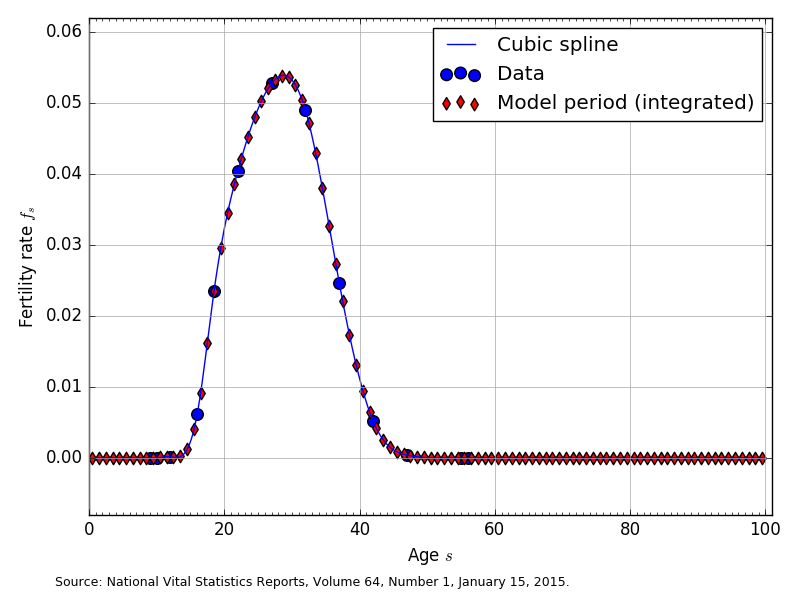
\includegraphics{./images/fert_rates.png}}}
  \end{figure}

  The large blue circles are the 2013 U.S. fertility rate data from \citet{MartinEtAl:2015}. These are 9 fertility rates $[0.3, 12.3, 47.1, 80.7, 105.5, 98.0, 49.3, 10.4, 0.8]$ that correspond to the midpoint ages of the following age (in years) bins $[10-14, 15-17, 18-19, 20-24, 25-29, 30-34, 35-39, 40-44, 45-49]$. In order to get our cubic spline interpolating function to fit better at the endpoints we added to fertility rates of zero to ages 9 and 10, and we added two fertility rates of zero to ages 55 and 56. The blue line in Figure \ref{FigFertRates} shows the cubic spline interpolated function of the data.

  The red diamonds in Figure \ref{FigFertRates} are the average fertility rate in age bins spanning households born at the beginning of period 1 (time = 0) and dying at the end of their 100th year. Let the total number of model years that a household lives be $E+S\leq 100$. Then the span from the beginning of period 1 (the beginning of year 0) to the end of period 100 (the end of year 99) is divided up into $E+S$ bins of equal length. We calculate the average fertility rate in each of the $E+S$ model-period bins as the average population-weighted fertility rate in that span. The red diamonds in Figure \ref{FigFertRates} are the average fertility rates displayed at the midpoint in each of the $E+S$ model-period bins.


\section{Mortality rates}\label{SecDemogMort}

  The mortality rates in our model $\rho_s$ are a one-period hazard rate and represent the probability of dying within one year, given that an household is alive at the beginning of period $s$. We assume that the mortality rates for each age cohort $\rho_s$ are constant across time. The infant mortality rate of $\rho_0=0.00587$ comes from the 2015 U.S. CIA World Factbook. Our data for U.S. mortality rates by age come from the Actuarial Life Tables of the U.S. Social Security Administration \citep[see][]{SocSec:2015}, from which the most recent mortality rate data is for 2011. Figure \ref{FigMortRates} shows the mortality rate data and the corresponding model-period mortality rates for $E+S=100$.

  \begin{figure}[htbp]\centering \captionsetup{width=4.0in}
    \caption{\label{FigMortRates}\textbf{Mortality rates by age ($\rho_s$) for $E+S=100$}}
    \fbox{\resizebox{4.0in}{3.0in}{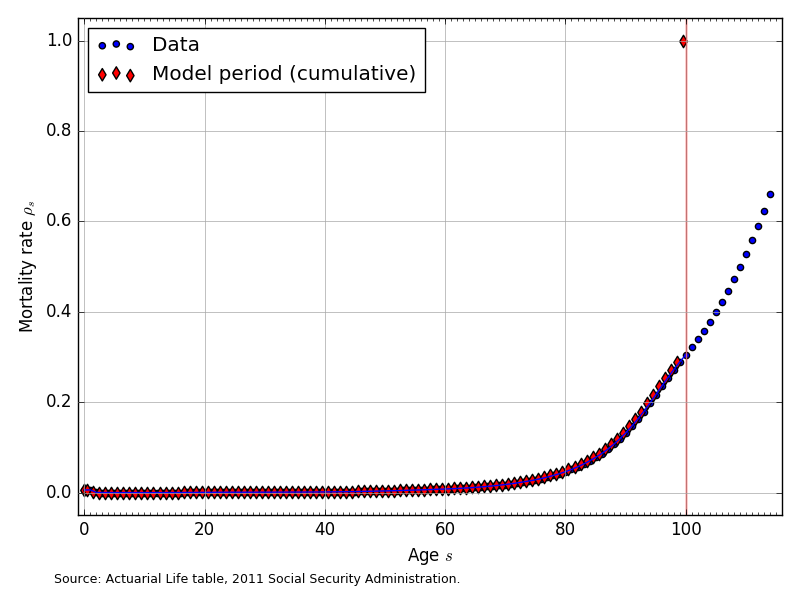
\includegraphics{./images/mort_rates.png}}}
  \end{figure}

  The mortality rates in Figure \ref{FigMortRates} are a population-weighted average of the male and female mortality rates reported in \citet{SocSec:2015}. Figure \ref{FigMortRates} also shows that the data provide mortality rates for ages up to 111-years-old. We truncate the maximum age in years in our model to 100-years old. In addition, we constrain the mortality rate to be 1.0 or 100 percent at the maximum age of 100.


\section{Immigration rates}\label{SecDemogImm}

  Because of the difficulty in getting accurate immigration rate data by age, we estimate the immigration rates by age in our model $i_s$ as the average residual that reconciles the current-period population distribution with next period's population distribution given fertility rates $f_s$ and mortality rates $\rho_s$. Solving equations \eqref{EqPopLawofmotion} for the immigration rate $i_s$ gives the following characterization of the immigration rates in given population levels in any two consecutive periods $\omega_{s,t}$ and $\omega_{s,t+1}$ and the fertility rates $f_s$ and mortality rates $\rho_s$.

  \begin{equation}\label{EqPopImmRates}
    \begin{split}
      i_1 &= \frac{\omega_{1,t+1} - (1 - \rho_0)\sum_{s=1}^{E+S}f_s\omega_{s,t}}{\omega_{1,t}}\quad\forall t \\
      i_{s+1} &= \frac{\omega_{s+1,t+1} - (1 - \rho_s)\omega_{s,t}}{\omega_{s+1,t}}\qquad\qquad\forall t\quad\text{and}\quad 1\leq s \leq E+S-1
    \end{split}
  \end{equation}

  \begin{figure}[htbp]\centering \captionsetup{width=4.0in}
    \caption{\label{FigImmRates}\textbf{Immigration rates by age ($i_s$), residual, $E+S=100$}}
    \fbox{\resizebox{4.0in}{3.0in}{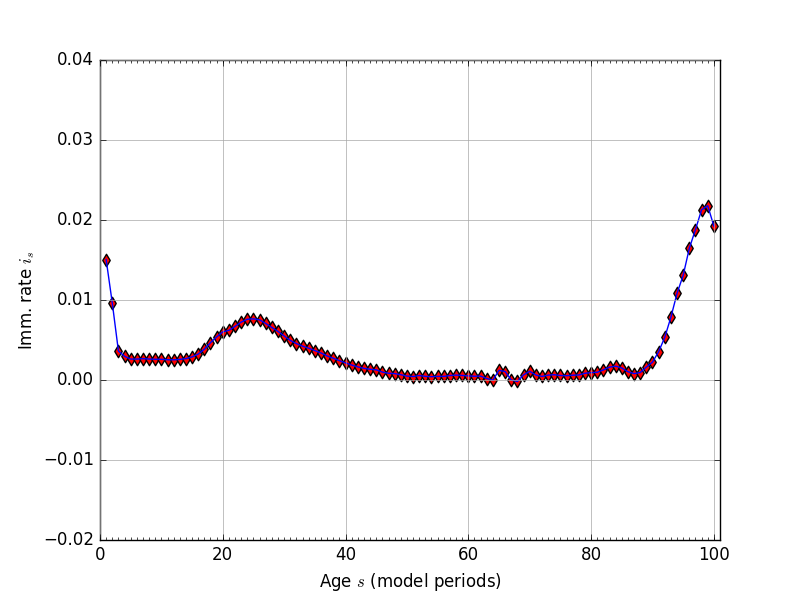
\includegraphics{./images/imm_rates_orig.png}}}
  \end{figure}

  We calculate our immigration rates for three different consecutive-year-periods of population distribution data (2010 through 2013). Our four years of population distribution by age data come from \citet{Census:2015}. The immigration rates $i_s$ that we use in our model are the the residuals described in \eqref{EqPopImmRates} averaged across the three periods. Figure \ref{FigImmRates} shows the estimated immigration rates for $E+S=100$ and given the fertility rates from Section \ref{SecDemogFert} and the mortality rates from Section \ref{SecDemogMort}.

  At the end of Section \ref{SecDemogPopSSTP}, we describe a small adjustment that we make to the immigration rates after a certain number of periods in order to make computation of the transition path equilibrium of the model compute more robustly.


\section{Population steady-state and transition path}\label{SecDemogPopSSTP}

  This model requires information about mortality rates $\rho_s$ in order to solve for the household's problem each period. It also requires the steady-state stationary population distribution $\bar{\omega}_{s}$ and population growth rate $\bar{g}_n$ as well as the full transition path of the stationary population distribution $\hat{\omega}_{s,t}$ and population grow rate $\tilde{g}_{n,t}$ from the current state to the steady-state. To solve for the steady-state and the transition path of the stationary population distribution, we write the stationary population dynamic equations \eqref{EqPopLawofmotionStat} and their matrix representation \eqref{EqPopLOMstatmat}.
  \begin{equation}\label{EqPopLawofmotionStat}
    \begin{split}
      \hat{\omega}_{1,t+1} &= \frac{(1-\rho_0)\sum_{s=1}^{E+S} f_s\hat{\omega}_{s,t} + i_1\hat{\omega}_{1,t}}{1+\tilde{g}_{n,t+1}}\quad\forall t \\
      \hat{\omega}_{s+1,t+1} &= \frac{(1 - \rho_s)\hat{\omega}_{s,t} + i_{s+1}\hat{\omega}_{s+1,t}}{1+\tilde{g}_{n,t+1}}\qquad\quad\:\forall t\quad\text{and}\quad 1\leq s \leq E+S-1
    \end{split}
  \end{equation}
  \begin{equation}\label{EqPopLOMstatmat}
    \begin{split}
      & \begin{bmatrix}
        \hat{\omega}_{1,t+1} \\ \hat{\omega}_{2,t+1} \\ \hat{\omega}_{2,t+1} \\ \vdots \\ \hat{\omega}_{E+S-1,t+1} \\ \hat{\omega}_{E+S,t+1}
      \end{bmatrix}= \frac{1}{1 + g_{n,t+1}} \times ... \\
      & \begin{bmatrix}
        (1-\rho_0)f_1+i_1 & (1-\rho_0)f_2 & (1-\rho_0)f_3 & \hdots & (1-\rho_0)f_{E+S-1} & (1-\rho_0)f_{E+S} \\
        1-\rho_1 & i_2 & 0 & \hdots & 0 & 0 \\
        0 & 1-\rho_2 & i_3 & \hdots & 0 & 0 \\
        \vdots & \vdots & \vdots & \ddots & \vdots & \vdots \\
        0 & 0 & 0 & \hdots & i_{E+S-1} & 0 \\
        0 & 0 & 0 & \hdots & 1-\rho_{E+S-1} & i_{E+S}
      \end{bmatrix}
      \begin{bmatrix}
        \hat{\omega}_{1,t} \\ \hat{\omega}_{2,t} \\ \hat{\omega}_{2,t} \\ \vdots \\ \hat{\omega}_{E+S-1,t} \\ \hat{\omega}_{E+S,t}
      \end{bmatrix}
    \end{split}
  \end{equation}
  We can write system \eqref{EqPopLOMstatmat} more simply in the following way.
  \begin{equation}\label{EqPopLOMstatmat2}
    \bm{\hat{\omega}}_{t+1} = \frac{1}{1+g_{n,t+1}}\bm{\Omega}\bm{\hat{\omega}}_t \quad\forall t
  \end{equation}
  The stationary steady-state population distribution $\bm{\bar{\omega}}$ is the eigenvector $\bm{\omega}$ with eigenvalue $(1+\bar{g}_n)$ of the matrix $\bm{\Omega}$ that satisfies the following version of \eqref{EqPopLOMstatmat2}.
  \begin{equation}\label{EqPopLOMss}
    (1+\bar{g}_n)\bm{\bar{\omega}} = \bm{\Omega}\bm{\bar{\omega}}
  \end{equation}

  \begin{proposition}
    If the age $s=1$ immigration rate is $i_1>-(1-\rho_0)f_1$ and the other immigration rates are strictly positive $i_s>0$ for all $s\geq 2$ such that all elements of $\bm{\Omega}$ are nonnegative, then there exists a unique positive real eigenvector $\bm{\bar{\omega}}$ of the matrix $\bm{\Omega}$, and it is a stable equilibrium.
  \end{proposition}

  \begin{proof}
    First, note that the matrix $\bm{\Omega}$ is square and non-negative.  This is enough for a general version of the Perron-Frobenius Theorem to state that a positive real eigenvector exists with a positive real eigenvalue. This is not yet enough for uniqueness. For it to be unique by a version of the Perron-Fobenius Theorem, we need to know that the matrix is irreducible. This can be easily shown. The matrix is of the form
    $$\bm{\Omega} =
    \begin{bmatrix}
      * & *  & * & \hdots & * & * & *\\
      * & * & 0 & \hdots & 0 & 0 & 0 \\
      0 & * & * & \hdots & 0 & 0 & 0 \\
      \vdots & \vdots & \vdots & \ddots & \vdots & \vdots & \vdots \\
      0 & 0 & 0 & \hdots & *  & * & 0 \\
      0 & 0 & 0 & \hdots & 0 & * & *
    \end{bmatrix}
    $$
    Where each * is strictly positive. It is clear to see that taking powers of the matrix causes the sub-diagonal positive elements to be moved down a row and another row of positive entries is added at the top. None of these go to zero since the elements were all non-negative to begin with.
    $$\bm{\Omega}^2 =
    \begin{bmatrix}
      * & *  & * & \hdots & * & * & *\\
      * & * & * & \hdots & * & * & * \\
      0 & * & * & \hdots & 0 & 0 & 0 \\
      \vdots & \vdots & \vdots & \ddots & \vdots & \vdots & \vdots \\
      0 & 0 & 0 & \hdots & *  & * & 0 \\
      0 & 0 & 0 & \hdots & 0 & * & *
    \end{bmatrix}; ~~~
    \bm{\Omega}^{S+E-1} =
    \begin{bmatrix}
      * & *  & * & \hdots & * & * & *\\
      * & * & * & \hdots & * & * & * \\
      * & * & * & \hdots & * & * & * \\
      \vdots & \vdots & \vdots & \ddots & \vdots & \vdots & \vdots \\
      * & * & * & \hdots & *  & * & * \\
      0 & 0 & 0 & \hdots & 0 & * & *
    \end{bmatrix}
    $$
    $$\bm{\Omega}^{S+E} =
    \begin{bmatrix}
      * & *  & * & \hdots & * & * & *\\
      * & * & * & \hdots & * & * & * \\
      * & * & * & \hdots & * & * & * \\
      \vdots & \vdots & \vdots & \ddots & \vdots & \vdots & \vdots \\
      * & * & * & \hdots & * & * & * \\
      * & * & * & \hdots & * & * & *
    \end{bmatrix}
    $$
    Existence of an $m \in \mathbb N $ such that $\left(\bf\Omega^m\right)_{ij} \neq 0 ~~ ( > 0)$ is one of the definitions of an irreducible (primitive) matrix. It is equivalent to saying that the directed graph associated with the matrix is strongly connected. Now the Perron-Frobenius Theorem for irreducible matrices gives us that the equilibrium vector is unique.

    We also know from that theorem that the eigenvalue associated with the positive real eigenvector will be real and positive. This eigenvalue, $p$, is the Perron eigenvalue and it is the steady state population growth rate of the model. By the PF Theorem for irreducible matrices, $| \lambda_i | \leq p$ for all eigenvalues $\lambda_i$ and there will be exactly $h$ eigenvalues that are equal, where $h$ is the period of the matrix. Since our matrix $\bf\Omega$ is aperiodic, the steady state growth rate is the unique largest eigenvalue in magnitude. This implies that almost all initial vectors will converge to this eigenvector under iteration.
  \end{proof}

  For a full treatment and proof of the Perron-Frobenius Theorem, see \citet{Suzumura:1983}. Because the population growth process is exogenous to the model, we calibrate it to annual age data for age years $s=1$ to $s=100$.

  Figure \ref{FigOrigVsFixSSpop} shows the steady-state population distribution $\bm{\bar{\omega}}$ and the population distribution after 120 periods $\bm{\hat{\omega}}_{120}$. Although the two distributions look very close to each other, they are not exactly the same.

  \begin{figure}[htbp]\centering \captionsetup{width=4.0in}
    \caption{\label{FigOrigVsFixSSpop}\textbf{Theoretical steady-state population distribution vs. population distribution at period $t=120$}}
    \fbox{\resizebox{4.0in}{3.0in}{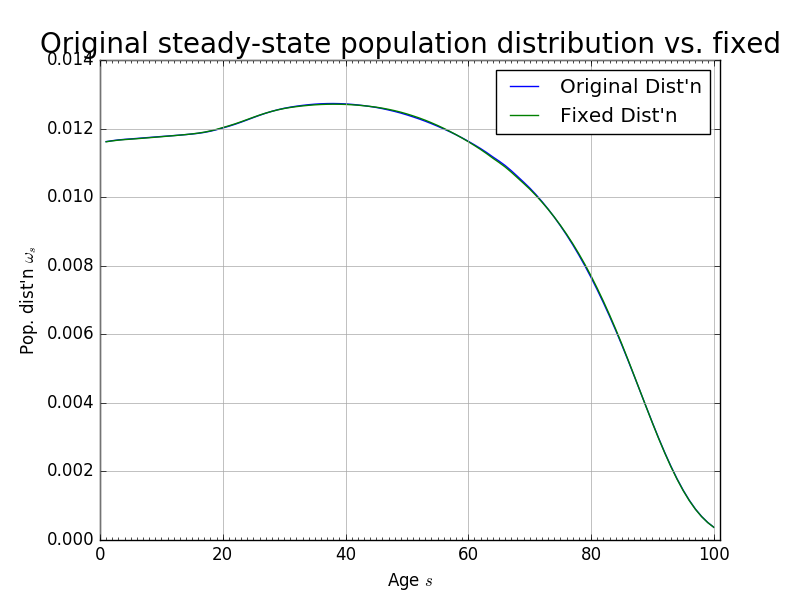
\includegraphics{./images/OrigVsFixSSpop.png}}}
  \end{figure}

  Further, we find that the maximum absolute difference between the population levels $\hat{\omega}_{s,t}$ and $\hat{\omega}_{s,t+1}$ was $1.3852\times 10^{-5}$ after 160 periods. That is to say, that after 160 periods, given the estimated mortality, fertility, and immigration rates, the population has not achieved its steady state. For convergence in our solution method over a reasonable time horizon, we want the population to reach a stationary distribution after $T$ periods. To do this, we artificially impose that the population distribution in period $t=120$ is the steady-state. As can be seen from Figure \ref{FigOrigVsFixSSpop}, this assumption is not very restrictive. Figure \ref{FigImmRateChg} shows the change in immigration rates that would make the period $t=120$ population distribution equal be the steady-state. The maximum absolute difference between any two corresponding immigration rates in Figure \ref{FigImmRateChg} is 0.0028.

  \begin{figure}[htbp]\centering \captionsetup{width=4.0in}
    \caption{\label{FigImmRateChg}\textbf{Original immigration rates vs. adjusted immigration rates to make fixed steady-state population distribution}}
    \fbox{\resizebox{4.0in}{3.0in}{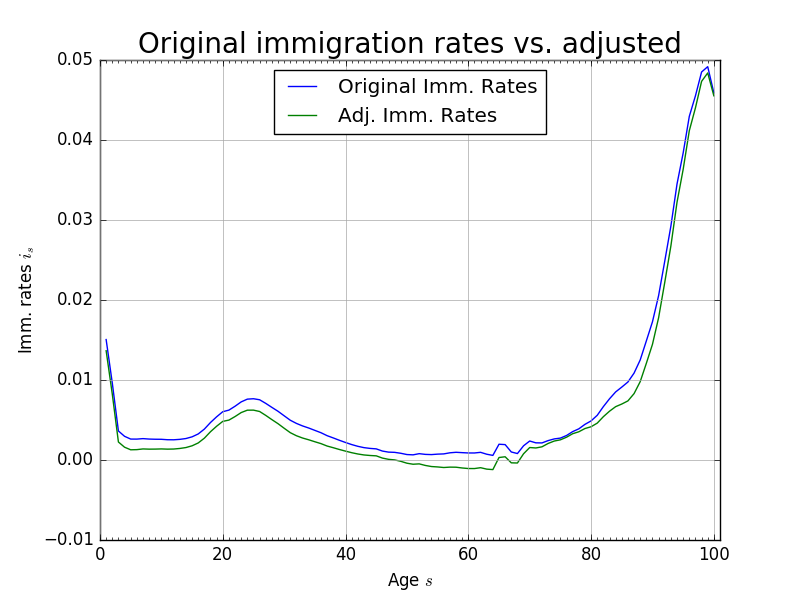
\includegraphics{./images/OrigVsAdjImm.png}}}
  \end{figure}

  The most recent year of population data come from \citet{Census:2015} population estimates for both sexes for 2013. We those data and use the population transition matrix \eqref{EqPopLOMstatmat2} to age it to the current model year of 2015. We then use \eqref{EqPopLOMstatmat2} to generate the transition path of the population distribution over the time period of the model. Figure \ref{FigPopDistPath} shows the progression from the 2013 population data to the fixed steady-state at period $t=120$. The time path of the growth rate of the economically active population $\tilde{g}_{n,t}$ is shown in Figure \ref{FigGrowthPath}.

  \begin{figure}[htbp]\centering \captionsetup{width=4.0in}
    \caption{\label{FigPopDistPath}\textbf{Stationary population distribution at periods along transition path}}
    \fbox{\resizebox{4.0in}{3.0in}{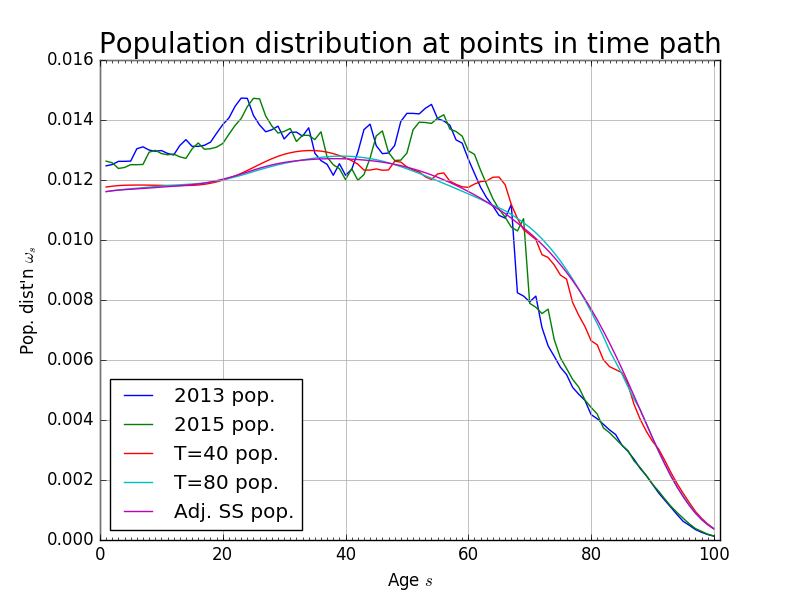
\includegraphics{./images/PopDistPath.png}}}
  \end{figure}

  \begin{figure}[htbp]\centering \captionsetup{width=4.0in}
    \caption{\label{FigGrowthPath}\textbf{Time path of the population growth rate $\tilde{g}_{n,t}$}}
    \fbox{\resizebox{4.0in}{3.0in}{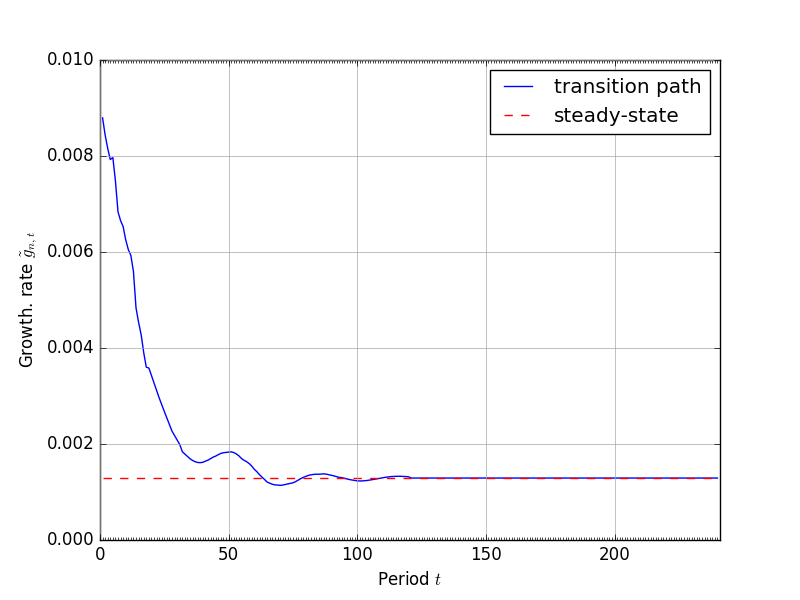
\includegraphics{./images/GrowthPath.png}}}
  \end{figure}

  \chapter{Lifetime Earnings Profiles}\label{Chap_LfEarn}
    %!TEX root = ../OGUSAdoc.tex

Among households in \ogindia, we model both age heterogeneity and within-age ability heterogeneity. We use this ability or productivity heterogeneity to generate the income heterogeneity that we see in the data.

Differences among workers' productivity in terms of ability is one of the key dimensions of heterogeneity to model in a micro-founded macroeconomy. In this chapter, we characterize this heterogeneity as deterministic lifetime productivity paths to which new cohorts of agents in the model are randomly assigned. In \ogindia, households' labor income comes from the equilibrium wage and the agent's endogenous quantity of labor supply. In this section, we augment the labor income expression with an individual productivity $e_{j,s}$, where $j$ is the index of the ability type or path of the individual and $s$ is the age of the individual with that ability path.
\begin{equation}\tag{\ref{EqTaxCalcLabInc}}
  \text{labor income:}\quad x_{j,s,t}\equiv w_t e_{j,s}n_{j,s,t} \quad\forall j,t \quad\text{and}\quad E+1\leq s\leq E+S
\end{equation}
In this specification, $w_t$ is an equilibrium wage representing a portion of labor income that is common to all workers. Individual quantity of labor supply is $n_{j,s,t}$, and $e_{j,s}$ represents a labor productivity factor that augments or diminishes the productivity of a worker's labor supply relative to average productivity.

We calibrate deterministic ability paths such that each lifetime income group has a different life-cycle profile of earnings. The distribution on income and wealth are often focal components of macroeconomic models. As such, we use a calibration of deterministic lifetime ability paths from \citet{DeBackerEtAl:2017b} that can represent U.S. earners in the top 1\% of the distribution of lifetime income. \citet{PikettySaez:2003} show that income and wealth attributable to these households has shown the greatest growth in recent decades. The data come from the U.S. Internal Revenue Services's (IRS) Statistics of Income program (SOI) Continuous Work History Sample (CWHS). \citet{DeBackerEtAl:2017b} match the SOI data with Social Security Administration (SSA) data on age and Current Population Survey (CPS) data on hours in order to generate a non-top-coded measure of hourly wage.

\begin{figure}[htbp]\centering \captionsetup{width=4.0in}
  \caption{\label{FigLogAbil}\textbf{Exogenous life cycle income ability paths $\log(e_{j,s})$ with $S=80$ and $J=7$}}
  \fbox{\resizebox{4.0in}{3.0in}{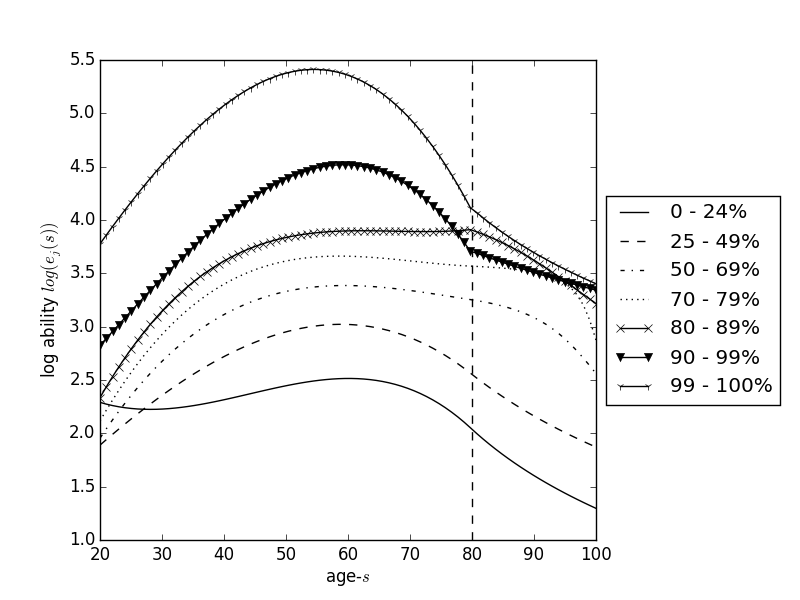
\includegraphics{images/ability_log_2D.png}}}
\end{figure}

Figure \ref{FigLogAbil} shows a calibration for $J=7$ deterministic lifetime ability paths $e_{j,s}$ corresponding to labor income percentiles $\bm{\lambda}=[0.25, 0.25, 0.20, 0.10, 0.10, 0.09, 0.01]$. Because there are few individuals above age 80 in the data, \citet{DeBackerEtAl:2017b} extrapolate these estimates for model ages 80-100 using an arctan function.

We calibrate the model such that each lifetime income group has a different life-cycle profile of earnings. Since the distribution on income and wealth are key aspects of our model, we calibrate these processes so that we can represent earners in the top 1 percent of the distribution of lifetime income. It is income and wealth attributable to these households that has shown the greatest growth in recent decades (see, for example, \citet{PikettySaez:2003}). In order to have observations on the earnings of those at very top of the distribution that are not subject to top-coding we use data from the Internal Revenue Services's (IRS) Statistics of Income program (SOI).


\section{Continuous Work History Sample}\label{SecLFEarnCWHS}

  The SOI data we draw from are the Continuous Work History Sample (CWHS).  From this CWHS, we use a panel that is a 1-in-5000 random sample of tax filers from 1991 to 2009.  For each filer-year observation we are able to observe detailed information reported on Form 1040 and the associated forms and schedules.  We are also able to merge these tax data with Social Security Administration (SSA) records to get information on the age and gender of the primary and secondary filers.  Our model variable of effective labor units maps into wage rates, because the market wage rate in the model, $w_{t}$, is constant across households.  Earnings per hour thus depend upon effective labor units and equal $e_{j,s,t}\times w_{t}$ for household in lifetime income group $j$, with age $s$, in year $t$.  Income tax data, however, do not contain information on hourly earnings or hours works.  Rather, we only observe total earned income (wage and salaries plus self-employment income) over the tax year.  In order to find hourly earnings for tax filers, we use an imputation procedure.  This is described in detail in \citet{DeBackerRamnath:2017}.  The methodology applies an imputation for hours worked for a filing unit based on a model of hours worked for a filing unit estimated from the Current Population Survey (CPS) for the years 1992-2010.\footnote{The CPS survey asks retrospective questions about income in the last year and average hours worked per week (and weeks worked) in the last year).  Therefore, these CPS surveys line up with tax years 1991-2009.} We then use the imputed hours to calculate hourly earnings rates for tax filing units in the CWHS.

  We exclude from our sample filer-year observations with earned income (wages and salaries plus business income) of less than \$1,250. We further exclude those with positive annual wages, but with hourly wages below \$5.00 (in 2005\$). We also drop one observation where the hourly wage rate exceeds \$25,000.\footnote{This threshold is equivalent to \$50 million of wage income in one year at full time (40 hours per week) of work.} Economic life in the model runs from age 21 to 100. Our data have few observations on filers with ages exceeding 80 years old. Our sample is therefore restricted to those from ages 21 to 80. After these restrictions, our final sample size is 333,381 filer-year observations.


\section{Lifetime Income}\label{SecLFearnLifInc}

  In our model, labor supply and savings, and thus lifetime income, are endogenous. We therefore define lifetime income as the present value of lifetime labor endowments and not the value of lifetime labor earnings. Note that our data are at the tax filing unit.  We take this unit to be equivalent to a household.  Because of differences in household structure (i.e., singles versus couples), our definition of lifetime labor income will be in per adult terms.  In particular, for filing units with a primary and secondary filer, our imputed wage represents the average hourly earnings between the two. When calculating lifetime income we assign single and couple households the same labor endowment.  This has the effect of making our lifetime income metric a per adult metric, there is therefore not an over-representation of couple households in the higher lifetime income groups simply because their time endowment is higher than for singles. We use the following approach to measure the lifetime income.

  First, since our panel data do not allow us to observe the complete life cycle of earnings for each household (because of sample attrition, death or the finite sample period of the data), we use an imputation to estimate wages in the years of the household's economic life for which they do not appear in the CWHS. To do this, we estimate the following equation, separately by household type (where household types are single male, single female, couple with male head, or couple with female head):
  \begin{equation}\label{eqn:wage_step1}
    ln(w_{i,t}) = \alpha_{i} + \beta_{1}age_{i,t} + \beta_{2}age_{i,t}^{2} + \beta_{3}*age_{i,t}^{3} + \varepsilon_{i,t}
  \end{equation}

  \begin{table}[htbp]\centering\captionsetup{width=5.8in}
    \caption{\label{tab:wage_step1}\textbf{Initial Log Wage Regressions}}
    \begin{threeparttable}
    \begin{tabular}{>{\scriptsize}l |>{\scriptsize}c >{\scriptsize}c >{\scriptsize}c >{\scriptsize}c}
    \hline\hline
    \multicolumn{1}{c}{\scriptsize{Dependent}} & Single & Single & Married, & Married, \\[-2mm]
    \multicolumn{1}{c}{\scriptsize{variables}}  & males & females & male head  & female head \\
    \hline
    $Age$ & 0.177*** & 0.143*** & 0.134*** & 0.065** \\
          & (0.006) & (0.005) & (0.004) & (0.027) \\
    $Age^{2}$ & -0.003*** & -0.002*** & -0.002*** & -0.000 \\
              & (0.000) & (0.000) & (0.000) & (0.001) \\
    $Age^{3}$ & 0.000*** & 0.000*** & 0.000*** & 0.000 \\
              & (0.000) & (0.000) & (0.000) & (0.000) \\
    Constant & -0.839*** & -0.648*** & -0.042 & 1.004*** \\
             & (0.072) & (0.070) & (0.058) & (0.376) \\
    \hline
    Adj $R^{2}$  & -0.007 & 0.011 & -0.032 & -0.324 \\
    Observations & 88,833 & 96,670 & 141,564 & 6,314 \\
    \hline\hline
    \end{tabular}
    \begin{tablenotes}
      \scriptsize{\item[]Source: CWHS data, 1991 -- 2009.
      \item[**]Significant at the 5 percent level ($p<0.05$).
      \item[***]Significant at the 1 percent level ($p<0.01$).}
    \end{tablenotes}
    \end{threeparttable}
  \end{table}

  The parameter estimates, including the household fixed effects, from Equation \ref{eqn:wage_step1} are shown in Table \ref{tab:wage_step1}. These estimates are then used to impute values for log wages in years of each households' economic life for which we do not have data.  This creates a balanced panel of log wages of households with heads aged 21 to 80. The actual and imputed wage values are then used to calculate the net present value of lifetime labor endowments per adult for each household. Specifically, we define lifetime income for household $i$ as:

  \begin{equation}\label{eqn:LI}
    LI_{i} = \sum_{t=21}^{80}\left(\frac{1}{1+r}\right)^{t-21}(w_{i,t}*4000)
  \end{equation}

  \noindent\noindent Note that households are all have the same time endowment in each year (4000 hours).  Thus the amount of the time endowment scales lifetime income up or down, but does not change the lifetime income of one household relative to another. This is not the case with the interest rate, $r$, which we fix at 4\%. Changes in the interest rate differentially impact the lifetime income calculation for different individuals because they may face different earnings profiles. For example, a higher interest rate would reduced the discounted present value of lifetime income for those individuals whose wage profiles peaked later in their economic life by a larger amount than it would reduce the discounted present value of lifetime income for individuals whose wage profiles peaked earlier.


\section{Profiles by Lifetime Income}

  With observations of lifetime income for each household, we next sort households and find the percentile of the lifetime income distribution that each household falls in.  With these percentiles, we create our lifetime income groupings.
  \begin{equation}\label{EqLfEarnLambda_j}
    \lambda_{j}=[0.25, 0.25, 0.2, 0.1, 0.1, 0.09, 0.01]
  \end{equation}
  That is, lifetime income group one includes those in below the 25th percentile, group two includes those from the 25th to the median, group three includes those from the median to the 70th percentile, group four includes those from the 70th to the 80th percentile, group 5 includes those from the 80th to 90th percentile, group 6 includes those from the 90th to 99th percentile, and group 7 consists of the top one percent in the lifetime income distribution.  Table \ref{tab:li_group_stats} presents descriptive statistics for each of these groups.

  \begin{table}[htbp] \centering \captionsetup{width=6.0in}
  \caption{\label{tab:li_group_stats}\textbf{Descriptive Statistics by Lifetime Income Category}}
    \begin{threeparttable}
    \begin{tabular}{>{\scriptsize}l |>{\scriptsize}r >{\scriptsize}r >{\scriptsize}r >{\scriptsize}r >{\scriptsize}r >{\scriptsize}r >{\scriptsize}r >{\scriptsize}r}
      \hline\hline
      \multicolumn{1}{c}{\scriptsize{Lifetime Income}} & & & & & & & & \\
      \multicolumn{1}{c}{\scriptsize{Category:}} & \multicolumn{1}{c}{\scriptsize{1}} & \multicolumn{1}{c}{\scriptsize{2}} & \multicolumn{1}{c}{\scriptsize{3}} & \multicolumn{1}{c}{\scriptsize{4}} & \multicolumn{1}{c}{\scriptsize{5}} & \multicolumn{1}{c}{\scriptsize{6}} & \multicolumn{1}{c}{\scriptsize{7}} & \multicolumn{1}{c}{\scriptsize{All}} \\
      \hline
      Percentiles & 0-25  & 25-50 & 50-70 & 70-80 & 80-90 & 90-99 & 99-100 & 0-100 \\
      Observations & 65,698 & 101,484 & 74,253 & 33,528 & 31,919 & 24,370 & 2,129 & 333,381 \\
      Fraction Single & & & & & & & & \\
      \ \ \ Females & 0.30  & 0.24  & 0.25  & 0.32  & 0.38  & 0.40  & 0.22  & 0.28 \\
      \ \ \  Males & 0.18  & 0.22  & 0.30  & 0.35  & 0.38  & 0.37  & 0.20  & 0.26 \\
      Fraction Married & & & & & & & & \\
      \ \ \ Female Head & 0.08  & 0.00  & 0.00  & 0.00  & 0.00  & 0.00  & 0.00  & 0.02 \\
      \ \ \ Male Head & 0.45  & 0.53  & 0.45  & 0.32  & 0.23  & 0.23  & 0.57  & 0.39 \\
      Mean: & & & & & & & & \\
      Age, Primary & 51.72 & 44.15 & 38.05 & 34.09 & 31.53 & 30.79 & 40.17 & 39.10 \\
      Hourly Wage & 11.60 & 16.98 & 20.46 & 23.04 & 26.06 & 40.60 & 237.80 & 21.33 \\
      Annual Wages & 25,178 & 44,237 & 54,836 & 57,739 & 61,288 & 92,191 & 529,522 & 51,604 \\
      Lifetime Income & 666,559 & 1,290,522 & 1,913,029 & 2,535,533 & 3,249,287 & 5,051,753 & 18,080,868 & 2,021,298 \\
      \hline\hline
    \end{tabular}%
    \begin{tablenotes}
      \tiny{\item[*] CWHS data, 1991-2009, all nominal values in 2005\$.}
    \end{tablenotes}
    \end{threeparttable}
  \end{table}

  To get a life-cycle profile of effective labor units for each group, we estimate the wage profile for each lifetime income group.  We do this by estimating the following regression model separately for each lifetime income group using data on actual (not imputed) wages:
  \begin{equation}\label{eqn:wage_profile}
    ln(w_{i,t})=\alpha +  \beta_{1}age_{i,t} + \beta_{2}age_{i,t}^{2} + \beta_{3}*age_{i,t}^{3}+ \varepsilon_{i,t}
  \end{equation}
  The estimated parameters from equation \eqref{eqn:wage_profile} are given in Table \ref{tab:wage_profiles}. The life-cycle earnings profiles implied by these parameters are plotted in Figure \ref{FigLogAbil}. Note that there are few individuals above age 80 in the data. To extrapolate these estimates for model ages 80-100, we use an arctan function of the following form:
  \begin{equation}\label{EqLfEarnArctan}
    y = \left(\frac{-a}{\pi}\right)*arctan(bx+c)+\frac{a}{2}
  \end{equation}
  where $x$ is age, and $a$, $b$, and $c$ are the parameters we search over for the best fit of the function to the following three criteria: 1) the value of the function should match the value of the data at age 80 2) the slope of the arctan should match the slope of the data at age 80 and 3) the value of the function should match the value of the data at age 100 times a constant.  This constant is .5 for all lifetime income groups, except the 2nd highest ability is .7 (otherwise, the 2nd highest has a lower income than the 3rd highest ability group in the last few years).

  \begin{table}[htbp] \centering \captionsetup{width=6.0in}
  \caption{\label{tab:wage_profiles}\textbf{Log Wage Regressions, by Lifetime Income Group}}
    \begin{threeparttable}
    \begin{tabular}{>{\scriptsize}l |>{\scriptsize}c >{\scriptsize}c >{\scriptsize}c >{\scriptsize}c |>{\scriptsize}c}
      \hline\hline
      \multicolumn{1}{c}{\scriptsize{Lifetime}} & & & & & \\
      \multicolumn{1}{c}{\scriptsize{income groups}}   & & & & & \\
      \multicolumn{1}{c}{\scriptsize{(percentiles)}} & Constant & $Age$ & $Age^2$ & $Age^3$ & Observations \\
      \hline
      0 to 25 & 3.41000000*** & -0.09720122*** & 0.00247639*** & -0.00001842*** & 65,698 \\
              & (0.08718100) & (0.00543339) & (0.00010901) & (0.00000071) &  \\
      25 to 50 & 0.69689692*** & 0.05995294*** & -0.00004086 & -0.00000521*** & 101,484 \\
            & (0.05020758) & (0.00345549) & (0.00007627) & (0.00000054) &  \\
      50 to 70 & -0.78761958*** & 0.17654618*** & -0.00240656*** & 0.00001039*** & 74,253 \\
               & (0.04519637) & (0.00338371) & (0.00008026) & (0.00000061) &  \\
      70 to 80 & -1.11000000*** & 0.21168263*** & -0.00306555*** & 0.00001438*** & 33,528 \\
            & (0.06838352) & (0.00530190) & (0.00012927) & (0.00000099) &  \\
      80 to 90  & -0.93939272*** & 0.21638731*** & -0.00321041*** & 0.00001579*** & 31,919 \\
            & (0.08333727) & (0.00664647) & (0.00016608) & (0.00000130) &  \\
      90 to 99 & 1.60000000*** & 0.04500235*** & 0.00094253*** & -0.00001470*** & 24,370 \\
            & (0.11723131) & (0.00931334) & (0.00022879) & (0.00000176) &  \\
      99 to 100 & 1.89000000*** & 0.09229392** & 0.00012902 & -0.00001169* & 2,129 \\
            & (0.50501510) & (0.03858202) & (0.00090072) & (0.00000657) &  \\
      \hline\hline
    \end{tabular}
    \begin{tablenotes}
      \scriptsize{\item[]Source: CWHS data, 1991 -- 2009.
      \item[*]Significant at the 10 percent level ($p<0.10$).
      \item[**]Significant at the 5 percent level ($p<0.05$).
      \item[***]Significant at the 1 percent level ($p<0.01$).}
    \end{tablenotes}
    \end{threeparttable}
  \end{table}

  \chapter{Households}\label{Chap_House}
    %!TEX root = ../OGUSAdoc.tex

In this chapter, we describe what is arguably the most important economic agent in the \ogindia model: the household. We model households in \ogindia rather than individuals, because we want to abstract from the concepts of gender, marital status, and number of children. Furthermore, the household is the usual unit of account in tax data. Because \ogindia is primarily a fiscal policy model using U.S. data, it is advantageous to have the most granular unit of account be the household.


\section{Budget Constraint}\label{SecHHBC}

  We described the derivation and dynamics of the population distribution in Chapter \ref{Chap_Demog}. A measure $\omega_{1,t}$ of households is born each period, become economically relevant at age $s=E+1$ if they survive to that age, and live for up to $E+S$ periods ($S$ economically active periods), with the population of age-$s$ individuals in period $t$ being $\omega_{s,t}$. Let the age of a household be indexed by $s = \{1,2,...E+S\}$.

  At birth, each household age $s=1$ is randomly assigned one of $J$ ability groups, indexed by $j$. Let $\lambda_j$ represent the fraction of individuals in each ability group, such that $\sum_j\lambda_j=1$. Note that this implies that the distribution across ability types in each age is given by $\bm{\lambda}=[\lambda_1,\lambda_2,...\lambda_J]$. Once an household is born and assigned to an ability type, it remains that ability type for its entire lifetime. This is deterministic ability heterogeneity as described in Chapter \ref{Chap_LfEarn}. Let $e_{j,s}>0$ be a matrix of ability-levels such that an individual of ability type $j$ will have lifetime abilities of $[e_{j,1},e_{j,2},...e_{j,E+S}]$. The budget constraint for the age-$s$ household in lifetime income group $j$ at time $t$ is the following,
  \begin{equation}\label{EqHHBC}
    \begin{split}
      c_{j,s,t} + b_{j,s+1,t+1} &= (1 + r_{t})b_{j,s,t} + w_t e_{j,s} n_{j,s,t} + \zeta_{j,s}\frac{BQ_t}{\lambda_j\omega_{s,t}} + \eta_{j,s,t}\frac{TR_{t}}{\lambda_j\omega_{s,t}} - T_{s,t}  \\
      &\quad\forall j,t\quad\text{and}\quad s\geq E+1 \quad\text{where}\quad b_{j,E+1,t}=0\quad\forall j,t
    \end{split}
  \end{equation}
  where $c_{j,s,t}$ is consumption, $b_{j,s+1,t+1}$ is savings for the next period, $r_t$ is the interest rate (return on savings), $b_{j,s,t}$ is current period wealth (savings from last period), $w_t$ is the wage, and $n_{j,s,t}$ is labor supply.

  The next term on the right-hand-side of the budget constraint \eqref{EqHHBC} represents the portion of total bequests $BQ_t$ that go to the age-$s$, income-group-$j$ household. Let $\zeta_{j,s}$ be the fraction of total bequests $BQ_t$ that go to the age-$s$, income-group-$j$ household, such that $\sum_{s=E+1}^{E+S}\sum_{j=1}^J\zeta_{j,s}=1$. We must divide that amount by the population of $(j,s)$ households $\lambda_j\omega_{s,t}$. Chapter \ref{Chap_Beq} details how to calibrate the $\zeta_{j,s}$ values from consumer finance data.

  The last two terms on the right-hand-side of the budget constraint \eqref{EqHHBC} have to do with government transfers and taxes, respectively. $TR_{t}$ is total government transfers to households in period $t$ and $\eta_{j,s,t}$ is the percent of those transfers that go to households of age $s$ and lifetime income group $j$ such that $\sum_{s=E+1}^{E+S}\sum_{j=1}^J\eta_{j,s,t}=1$. This term is divided by the population of type $(j,s)$ households. We assume government transfers to be lump sum, so they do not create any direct distortions to household decisions.

  The term $T_{s,t}$ is the total tax liability of the household. In contrast to government transfers $tr_{j,s,t}$, tax liability can be a function of labor income $(x_{j,s,t}\equiv w_t e_{j,s}n_{j,s,t})$ and capital income $(y_{j,s,t}\equiv r_t b_{j,s,t})$. The tax liability can, therefore, be a distortionary influence on household decisions. It becomes valuable to represent total tax liability as an effective tax rate $\tau^{etr}$ multiplied by total income,
  \begin{equation}\tag{\ref{EqTaxCalcLiabETR}}
    T_{s,t} = \tau^{etr}_{s,t}(x_{j,s,t}, y_{j,s,t})\left(x_{j,s,t} + y_{j,s,t}\right)
  \end{equation}
  where the effective tax rate can be a function of both labor income and capital income $\tau^{etr}(x,y)$. Chapter \ref{Chap_TaxCalc} details exactly how we estimate these tax functions from microsimulation model data.

  where many of the variables now have $j$ subscripts. The variables with three subscripts $(j,s,t)$ tell you to which ability type $j$ and age $s$ individual the variable belongs and in which period $t$.


\section{Elliptical Disutility of Labor Supply}\label{SecHHellipUtil}

  In \ogindia, the period utility function of each household is a function of consumption $c_{j,s,t}$, savings $b_{j,s+1,t+1}$, and labor supply $n_{j,s,t}$.\footnote{Savings enters the period utility function to provide a ``warm glow'' bequest motive.} We detail this utility function, its justification, and functional form in Section \ref{SecHHeulers}. With endogenous labor supply $n_{j,s,t}$, we must specify how labor enters an agent's utility function and what are the constraints. Assume that each household is endowed with a measure of time $\tilde{l}$ each period that it can choose to spend as either labor $n_{j,s,t}\in[0,\tilde{l}]$ or leisure $l_{j,s,t}\in[0,\tilde{l}]$.
  \begin{equation}\label{EqLabConstr}
    n_{j,s,t} + l_{j,s,t} = \tilde{l} \quad\forall s, t
  \end{equation}

  The functional form for the utility of leisure or the disutility of labor supply has important implications for the computational tractability of the model. One difference of the household's labor supply decision $n_{j,s,t}$ from the consumption decision $c_{j,s,t}$ is that the consumption decision only has a lower bound $c_{j,s,t}\geq 0$ whereas the labor supply decision has both upper and lower bounds $n_{j,s,t}\in[0,\tilde{l}]$. \citet{EvansPhillips:2017} show that many of the traditional functional forms for the disutility of labor---Cobb-Douglas, constant Frisch elasticty, constant relative risk aversion (CRRA)---do not have Inada conditions on both the upper and lower bounds of labor supply. To solve these in a heterogeneous agent model would require occasionally binding constraints, which is a notoriously difficult computational problem.

  \begin{figure}[htb]\centering \captionsetup{width=4.0in}
    \caption{\label{FigMDUcompar}\textbf{Comparison of CFE marginal disutility of leisure $\theta=0.9$ to fitted elliptical utility}}
    \fbox{\resizebox{4.0in}{3.2in}{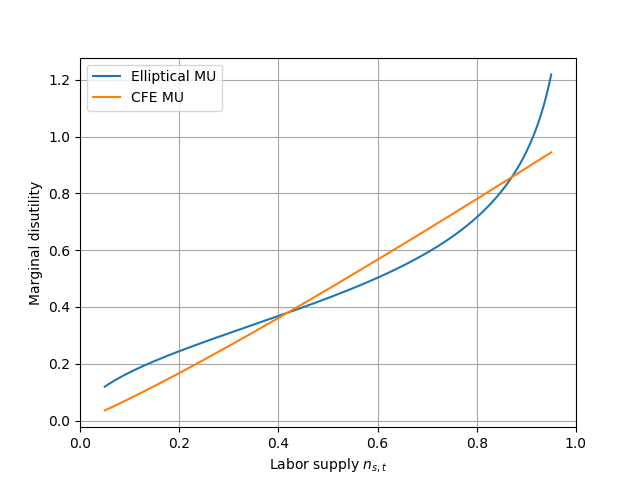
\includegraphics{images/EllipVsCFE_MargUtil.png}}}
  \end{figure}

  \citet{EvansPhillips:2017} propose using an equation for an ellipse to match the disutility of labor supply to whatever traditional functional form one wants. Our preferred specification in \ogindia is to fit an elliptical disutility of labor supply function to approximate a linearly separable constant Frisch elasticity (CFE) functional form. Let $v(n)$ be a general disutility of labor function. A CFE disutility of labor function is the following,
  \begin{equation}\label{EqCFE}
    v(n) \equiv \frac{n^{1+\frac{1}{\theta}}}{1+\frac{1}{\theta}}, \quad\theta > 0
  \end{equation}
  where $\theta>0$ represents the Frisch elasticity of labor supply. The elliptical disutility of labor supply functional form is the following,
  \begin{equation}\label{EqEllipDisut}
    v(n) = -b\left[1 - \left(\frac{n}{\tilde{l}}\right)^\upsilon\right]^{\frac{1}{\upsilon}}, \quad b,\upsilon>0
  \end{equation}
  where $b>0$ is a scale parameter and $\upsilon>0$ is a curvature parameter. This functional form satisfies both $v'(n)>0$ and $v''(n)>0$ for all $n\in(0,1)$. Further, it has Inada conditions at both the upper and lower bounds of labor supply $\lim_{n\rightarrow 0}v'(n) = 0$ and $\lim_{n\rightarrow \tilde{l}}v'(n) = -\infty$.

  Because it is the marginal disutility of labor supply that matters for household decision making, we want to choose the parameters of the elliptical disutility of labor supply function $(b,\upsilon)$ so that the elliptical marginal utilities match the marginal utilities of the CFE disutility of labor supply. Figure \ref{FigMDUcompar} shows the fit of marginal utilities for a Frisch elasticity of $\theta=0.9$ and a total time endowment of $\tilde{l}=1.0$. The estimated elliptical utility parameters in this case are $b=0.527$ and $\upsilon=1.497$.\footnote{\citet{Peterman:2016} shows that in a macro-model that has only an intensive margin of labor supply and no extensive margin and represents a broad composition of individuals supplying labor---such as \ogindia---a Frisch elasticity of around 0.9 is probably appropriate. He tests the implied macro elasticity when the assumed micro elasticities are small on the intensive margin but only macro aggregates---which include both extensive and intensive margin agents---are observed.}


\section{Optimality Conditions}\label{SecHHeulers}

  Households choose lifetime consumption $\{c_{j,s,t+s-1}\}_{s=1}^S$, labor supply $\{n_{j,s,t+s-1}\}_{s=1}^S$, and savings $\{b_{j,s+1,t+s}\}_{s=1}^{S}$ to maximize lifetime utility, subject to the budget constraints and non negativity constraints. The household period utility function is the following.
  \begin{equation}\label{EqHHPerUtil}
    \begin{split}
      u(c_{j,s,t},n_{j,s,t},b_{j,s+1,t+1}) &\equiv \frac{(c_{j,s,t})^{1-\sigma} - 1}{1-\sigma} + e^{g_y t(1-\sigma)}\chi^n_s\biggl(b\left[1 - \left(\frac{n_{j,s,t}}{\tilde{l}}\right)^\upsilon\right]^{\frac{1}{\upsilon}}\biggr) + \\
      &\chi^b_j \rho_s \frac{(b_{j,s+1,t+1})^{1-\sigma} - 1}{1-\sigma} \quad\forall j,t \quad\text{and}\quad E+1 \leq s \leq E+S
    \end{split}
  \end{equation}
  The period utility function \eqref{EqHHPerUtil} is linearly separable in $c_{j,s,t}$, $n_{j,s,t}$, and $b_{j,s+1,t+1}$. The first term is a constant relative risk aversion (CRRA) utility of consumption. The second term is the elliptical disutility of labor described in Section \ref{SecHHellipUtil}. The constant $\chi^n_s$ adjusts the disutility of labor supply relative to consumption and can vary by age $s$, which is helpful for calibrating the model to match labor market moments. See Chapter \ref{Chap_Calibr} for a discussion of the calibration.

  It is necessary to multiply the disutility of labor in \eqref{EqHHPerUtil} by $e^{g_y(1-\sigma)}$ because labor supply $n_{j,s,t}$ is stationary, but both consumption $c_{j,s,t}$ and savings $b_{j,s+1,t+1}$ are growing at the rate of technological progress (see Chapter \ref{Chap_Stnrz}). The $e^{g_y(1-\sigma)}$ term keeps the relative utility values of consumption, labor supply, and savings in the same units.

  The final term in the period utility function \eqref{EqHHPerUtil} is the ``warm glow'' bequest motive. It is a CRRA utility of savings, discounted by the mortality rate $\rho_s$.\footnote{See Section \ref{SecDemogMort} of Chapter \ref{Chap_Demog} for a detailed discussion of mortality rates in \ogindia.} Intuitively, it signifies the utility a household gets in the event that they don't live to the next period with probability $\rho_s$. It is a utility of savings beyond its usual benefit of allowing for more consumption in the next period. This utility of bequests also has constant $\chi^b_j$ which adjusts the utility of bequests relative to consumption and can vary by lifetime income group $j$. This is helpful for calibrating the model to match wealth distribution moments. See Chapter \ref{Chap_Calibr} for a discussion of the calibration. Note that any bequest before age $E+S$ is unintentional as it was bequeathed due an event of death that was uncertain. Intentional bequests are all bequests given in the final period of life in which death is certain $b_{j,E+S+1,t}$.

  The household lifetime optimization problem is to choose consumption $c_{j,s,t}$, labor supply $n_{j,s,t}$, and savings $b_{j,s+1,t+1}$ in every period of life to maximize expected discounted lifetime utility, subject to budget constraints and upper-bound and lower-bound constraints.
  \begin{align}
    &\max_{\{(c_{j,s,t}),(n_{j,s,t}),(b_{j,s+1,t+1})\}_{s=E+1}^{E+S}}\: \sum_{s=1}^S\beta^{s-1}\left[\Pi_{u=E+1}^{E+s}(1 - \rho_u)\right]u(c_{j,s,t+s-1},n_{j,s,t+s-1},b_{j,s+1,t+s}) \label{EqHHmaxprob} \\
    &\quad\text{s.t.}\quad c_{j,s,t} + b_{j,s+1,t+1} = (1 + r_{t})b_{j,s,t} + w_t e_{j,s} n_{j,s,t} + \zeta_{j,s}\frac{BQ_t}{\lambda_j\omega_{s,t}} + \eta_{j,s,t}\frac{TR_{t}}{\lambda_j\omega_{s,t}} - T_{s,t} \tag{\ref{EqHHBC}} \\
    &\qquad\text{and}\quad c_{j,s,t}\geq 0,\: n_{j,s,t} \in[0,\tilde{l}],\:\text{and}\: b_{j,1,t}=0 \quad\forall j, t, \:\text{and}\: E+1\leq s\leq E+S \nonumber
  \end{align}
  The nonnegativity constraint on consumption does not bind in equilibrium because of the Inada condition $\lim_{c\rightarrow 0}u_1(c,n,b') = \infty$, which implies consumption is always strictly positive in equilibrium $c_{j,s,t}>0$ for all $j$, $s$, and $t$. The warm glow bequest motive in \eqref{EqHHPerUtil} also has an Inada condition for savings at zero, so $b_{j,s,t}>0$ for all $j$, $s$, and $t$. This is an implicit borrowing constraint.\footnote{It is important to note that savings also has an implicit upper bound $b_{j,s,t}\leq k$ above which consumption would be negative in current period. However, this upper bound on savings in taken care of by the Inada condition on consumption.} And finally, as discussed in Section \ref{SecHHellipUtil}, the elliptical disutility of labor supply functional form in \eqref{EqHHPerUtil} imposes Inada conditions on both the upper and lower bounds of labor supply such that labor supply is strictly interior in equilibrium $n_{j,s,t}\in(0,\tilde{l})$ for all $j$, $s$, and $t$.

  The household maximization problem can be further reduced by substituting in the household budget constraint, which binds with equality. This simplifies the household's problem to choosing labor supply $n_{j,s,t}$ and savings $b_{j,s+1,t+1}$ every period to maximize lifetime discounted expected utility. The $2S$ first order conditions for every type-$j$ household that characterize the its $S$ optimal labor supply decisions and $S$ optimal savings decisions are the following.

  \begin{equation}\label{EqHHeul_n}
    \begin{split}
      &w_t e_{j,s}\bigl(1 - \tau^{mtrx}_{s,t}\bigr)(c_{j,s,t})^{-\sigma} = e^{g_y(1-\sigma)}\chi^n_{s}\biggl(\frac{b}{\tilde{l}}\biggr)\biggl(\frac{n_{j,s,t}}{\tilde{l}}\biggr)^{\upsilon-1}\Biggl[1 - \biggl(\frac{n_{j,s,t}}{\tilde{l}}\biggr)^\upsilon\Biggr]^{\frac{1-\upsilon}{\upsilon}} \\
      &\qquad\qquad\qquad\qquad\qquad\qquad\qquad\qquad\forall j,t, \quad\text{and}\quad E+1\leq s\leq E+S \\
    \end{split}
  \end{equation}

  \begin{equation}\label{EqHHeul_b}
    \begin{split}
      &(c_{j,s,t})^{-\sigma} = \chi^b_j\rho_s(b_{j,s+1,t+1})^{-\sigma} + \beta\bigl(1 - \rho_s\bigr)\Bigl(1 + r_{t+1}\bigl[1 - \tau^{mtry}_{s+1,t+1}\bigr]\Bigr)(c_{j,s+1,t+1})^{-\sigma} \\
      &\qquad\qquad\qquad\qquad\qquad\qquad\qquad\qquad\forall j,t, \quad\text{and}\quad E+1\leq s\leq E+S-1 \\
    \end{split}
  \end{equation}

  \begin{equation}\label{EqHHeul_bS}
    (c_{j,E+S,t})^{-\sigma} = \chi^b_j(b_{j,E+S+1,t+1})^{-\sigma} \quad\forall j,t \quad\text{and}\quad s = E+S
  \end{equation}



  The distortion of taxation on household decisions can be seen in Euler equations \eqref{EqHHeul_n} and \eqref{EqHHeul_b} in the terms that have a marginal tax rate $(1-\tau^{mtr})$. This comes from the expression for total tax liabilities as a function of the effective tax rate and total income as expressed in \eqref{EqTaxCalcLiabETR}. Using the chain rule, we can break up the derivatives of total tax liability with respect to $n_{j,s,t}$ and $b_{j,s,t}$, respectively, into simpler functions of marginal tax rates. We discuss this in more detail in Chapter \ref{Chap_TaxCalc}.

  \begin{equation}\tag{\ref{EqMTRx_derive}}
    \frac{\partial T_{s,t}}{\partial n_{j,s,t}}  = \frac{\partial T_{s,t}}{\partial w_t e_{j,s}n_{j,s,t}}\frac{\partial w_{t}e_{j,s}n_{j,s,t}}{\partial n_{j,s,t}} = \frac{\partial T_{s,t}}{\partial w_{t}e_{j,s}n_{j,s,t}}w_t e_{j,s} = \tau^{mtrx}_{s,t}w_t e_{j,s}
  \end{equation}

  \begin{equation}\tag{\ref{EqMTRy_derive}}
    \frac{\partial T_{s,t}}{\partial b_{j,s,t}} = \frac{\partial T_{s,t}}{\partial r_{t}b_{j,s,t}}\frac{\partial r_t b_{j,s,t}}{\partial b_{j,s,t}} = \frac{\partial T_{s,t}}{\partial r_t b_{j,s,t}}r_{t} = \tau^{mtry}_{s,t}r_t
  \end{equation}


\section{Expectations}\label{SecHHexp}

  To conclude the household's problem, we must make an assumption about how the age-$s$ household can forecast the time path of interest rates, wages, and total bequests $\{r_u, w_u, BQ_u\}_{u=t}^{t+S-s}$ over his remaining lifetime. As we will show in Chapters \ref{Chap_SSeqlb} and \ref{Chap_NSSeqlb}, the equilibrium interest rate $r_t$, wage $w_t$, and total bequests $BQ_t$ will be functions of the state vector $\bm{\Gamma}_t$, which turns out to be the entire distribution of savings at in period $t$.

  Define $\bm{\Gamma}_t$ as the distribution of household savings across households at time $t$.
  \begin{equation}\label{EqSavDist}
    \bm{\Gamma}_t \equiv \bigl\{b_{j,s,t}\bigr\}_{s=E+2}^{E+S} \quad\forall j,t
  \end{equation}
  Let general beliefs about the future distribution of capital in period $t+u$ be characterized by the operator $\Omega(\cdot)$ such that:
  \begin{equation}\label{EqBeliefs}
    \bm{\Gamma}^e_{t+u} = \Omega^u\left(\bm{\Gamma}_t\right) \quad \forall t, \quad u\geq 1
  \end{equation}
  where the $e$ superscript signifies that $\bm{\Gamma}^e_{t+u}$ is the expected distribution of wealth at time $t+u$ based on general beliefs $\Omega(\cdot)$ that are not constrained to be correct.\footnote{In Chapter \ref{Chap_NSSeqlb} we will assume that beliefs are correct (rational expectations) for the non-steady-state equilibrium in Definition \ref{DefNSSEql}.}

  \chapter{Calibrated Bequests}\label{Chap_Beq}
    %!TEX root = ../OGUSAdoc.tex

This chapter describes how we calibrate the distribution of total bequests $BQ_t$ to each living household of age $s$ and lifetime income group $j$. The matrix that governs this distribution $\zeta_{j,s}$ is seen in the household budget constraint \ref{EqHHBC}.

A large number of papers study the effects of different bequest motives and specifications on the distribution of wealth, though there is no consensus regarding the true bequest transmission process.\footnote{See \citet{DeNardiYang:2014}, \citet{DeNardi:2004}, \citet{Nishiyama:2002}, \citet{Laitner:2001}, \citet{GokhaleEtAl:2000}, \citet{GaleScholz:1994}, \citet{Hurd:1989}, \citet{VentiWise:1988}, \citet{KotlikoffSummers:1981}, and \citet{Wolff:2015}.}


\part{Firms Theory}\label{PartFirmTheory}
  \chapter{Firms}\label{Chap_Firms}
    %!TEX root = ../OGUSAdoc.tex

The production side of the \ogindia model is populated by a unit measure of identical perfectly competitive firms that rent capital $K_t$ and hire labor $L_t$ to produce output $Y_t$. Firms also face a flat corporate income tax $\tau^{corp}$ as well as a tax on the amount of capital they depreciate $\tau^\delta$.


\section{Production Function}\label{EqFirmsProdFunc}

  Firms produce output $Y_t$ using inputs of capital $K_t$ and labor $L_t$ according to a general constant elasticity (CES) of substitution production function,
  \begin{equation}\label{EqFirmsCESprodfun}
    Y_t = F(K_t, L_t) \equiv Z_t\biggl[(\gamma)^\frac{1}{\ve}(K_t)^\frac{\ve-1}{\ve} + (1-\gamma)^\frac{1}{\ve}(e^{g_y t}L_t)^\frac{\ve-1}{\ve}\biggr]^\frac{\ve}{\ve-1} \quad\forall t
  \end{equation}
  where $Z_t$ is an exogenous scale parameter (total factor productivity) that can be time dependent, $\gamma$ represents the capital share of income, and $\ve$ is the constant elasticity of substitution between capital and labor. We have included constant productivity growth $g_y$ as the rate of labor augmenting technological progress.

  A nice feature of the CES production function is that the Cobb-Douglas production function is a nested case for $\ve=1$.
  \begin{equation}\label{EqFirmsCDprodfun}
    Y_t = Z_t(K_t)^\gamma(e^{g_y t}L_t)^{1-\gamma} \quad\text{for}\quad \ve=1 \quad\forall t
  \end{equation}


\section{Optimality Conditions}\label{EqFirmsFOC}

  The profit function of the representative firm is the following.
  \begin{equation}\label{EqFirmsProfit}
    PR_t = (1 - \tau^{corp})\Bigl[F(K_t,L_t) - w_t L_t\Bigr] - \bigl(r_t + \delta\bigr)K_t + \tau^{corp}\delta^\tau K_t \quad\forall t
  \end{equation}
  Gross income for the firms is given by the production function $F(K,L)$ because we have normalized the price of the consumption good to 1. Labor costs to the firm are $w_t L_t$, and capital costs are $(r_t +\delta)K_t$. The per-period economic depreciation rate is given by $\delta$.

  Taxes enter the firm's profit function \eqref{EqFirmsProfit} in two places. The first is the corporate income tax rate $\tau^{corp}$, which is a flat tax on corporate income. As is the case in the U.S., corporate income is defined as gross income minus labor costs. This will cause the corporate tax to only distort the firms' capital demand decision.

  The next place where tax policy enters the profit function \eqref{EqFirmsProfit} is through a refund of a percent of depreciation costs $\delta^\tau$ refunded at the corporate income tax rate $\tau^{corp}$. When $\delta^\tau=0$, no depreciation expense is deducted from the firm's tax liability. When $\delta^\tau=\delta$, all economic depreciation is deducted from corporate income.

  Taking the derivative of the profit function \eqref{EqFirmsProfit} with respect to labor $L_t$ and setting it equal to zero and taking the derivative of the profit function with respect to capital $K_t$ and setting it equal to zero, respectively, characterizes the optimal labor and capital demands.
  \begin{align}
    w_t &= e^{g_y t}(Z_t)^\frac{\ve-1}{\ve}\left[(1-\gamma)\frac{Y_t}{e^{g_y t}L_t}\right]^\frac{1}{\ve} \quad\forall t \label{EqFirmFOC_L} \\
    r_t &= (1 - \tau^{corp})(Z_t)^\frac{\ve-1}{\ve}\left[\gamma\frac{Y_t}{K_t}\right]^\frac{1}{\ve} - \delta + \tau^{corp}\delta^\tau \quad\forall t \label{EqFirmFOC_K}
  \end{align}

  We discuss how to calibrate the values of $\tau^{corp}$ and $\tau^\delta$ from the \btax microsimulation model in Chapter \ref{Chap_BTax}.


\part{Government Theory}\label{PartGovtTheory}
  \chapter{Household Taxes and Tax-Calculator}\label{Chap_TaxCalc}
    %!TEX root = ../OGUSAdoc.tex

The government is not an optimizing agent in \ogindia. The government levies taxes on households, provides transfers to households, levies taxes on firms, spends resources on public goods, and makes rule-based adjustments to stabilize the economy in the long-run. The government can run budget deficits or surpluses in a given year and must, therefore, be able to accumulate debt or savings.

The government sector influences households through two terms in the budget constraint \eqref{EqHHBC}---government transfers $TR_{t}$ and through the total tax liability function $T_{s,t}$, which can be decomposed into the effective tax rate times total income \eqref{EqTaxCalcLiabETR}. In this chapter, we detail the household tax component of government activity $T_{s,t}$ in \ogindia, along with our method of incorporating detailed microsimulation data into a dynamic general equilibrium model.

Incorporating realistic tax and incentive detail into a general equilibrium model is notoriously difficult for two reasons. First, it is impossible in a dynamic general equilibrium model to capture all of the dimensions of heterogeneity on which the real-world tax rate depends. For example, a household's tax liability in reality depends on filing status, number of dependents, many types of income, and some characteristics correlated with age. A good heterogeneous agent DGE model tries to capture the most important dimensions of heterogeneity, and necessarily neglects the other dimensions.

The second difficulty in modeling realistic tax and incentive detail is the need for good microeconomic data on the individuals who make up the economy from which to simulate behavioral responses and corresponding tax liabilities and tax rates.

\ogindia follows the method of \citet{DeBackerEtAl:2017} of generating detailed tax data on effective tax rates and marginal tax rates for a sample of tax filers along with their respective income and demographic characteristics and then using that data to estimate parametric tax functions that can be incorporated into \ogindia.


\section{Effective and Marginal Tax Rates}\label{SecTaxCalcRateTheory}

  Before going into more detail regarding how we handle these two difficulties in \ogindia, we need to define some functions and make some notation. For notational simplicity, we will use the variable $x$ to summarize labor income, and we will use the variable $y$ to summarize capital income.
  \begin{align}
    x_{j,s,t} &\equiv w_{t}e_{j,s}n_{j,s,t} \quad\forall j, t \quad\text{and}\quad E+1\leq s\leq E+S \label{EqTaxCalcLabInc} \\
    y_{j,s,t} &\equiv r_{t}b_{j,s,t} \qquad\:\:\:\,\forall j, t \quad\text{and}\quad E+1\leq s\leq E+S \label{EqTaxCalcLabInc}
  \end{align}

  We can express total tax liability $T_{s,t}$ from the household budget constraint \eqref{EqHHBC} as an effective tax rate multiplied by total income.
  \begin{equation}\label{EqTaxCalcLiabETR}
    T_{s,t} = \tau^{etr}_{s,t}(x_{j,s,t}, y_{j,s,t})\left(x_{j,s,t} + y_{j,s,t}\right)
  \end{equation}
  Rearranging \eqref{EqTaxCalcLiabETR} gives the definition of an effective tax rate ($ETR$) as total tax liability divided by unadjusted gross income, or rather, total tax liability as a percent of unadjusted gross income.

  A marginal tax rate ($MTR$) is defined as the change in total tax liability from a small change income. In \ogindia, we differentiate between the marginal tax rate on labor income ($MTRx$) and the marginal tax rate on labor income ($MTRy$).
  \begin{align}
    \tau^{mtrx} &\equiv \frac{\partial T_{s,t}}{\partial w_t e_{j,s}n_{j,s,t}} = \frac{\partial T_{s,t}}{\partial x_{j,s,t}} \quad\forall j,t \quad\text{and}\quad E+1\leq s\leq E+S \label{EqTaxCalcMTRx} \\
    \tau^{mtry} &\equiv \frac{\partial T_{s,t}}{\partial r_t b_{j,s,t}} = \frac{\partial T_{s,t}}{\partial y_{j,s,t}} \qquad\quad\forall j,t \quad\text{and}\quad E+1\leq s\leq E+S \label{EqTaxCalcMTRy}
  \end{align}
  As we show in Section \ref{SecHHeulers}, the derivative of total tax liability with respect to labor supply $\frac{\partial T_{s,t}}{n_{j,s,t}}$ and the derivative of total tax liability next period with respect to savings $\frac{\partial T_{s+1,t+1}}{b_{j,s+1,t+1}}$ show up in the household Euler equations for labor supply \eqref{EqHHeul_n} and savings \eqref{EqHHeul_b}, respectively. It is valuable to be able to express those marginal tax rates, for which we have no data, as marginal tax rates for which we do have data. The following two expressions show how the marginal tax rates of labor supply can be expressed as the marginal tax rate on labor income times the household-specific wage and how the marginal tax rate of savings can be expressed as the marginal tax rate of capital income times the interest rate.
  \begin{equation}\label{EqMTRx_derive}
    \frac{\partial T_{s,t}}{\partial n_{j,s,t}}  = \frac{\partial T_{s,t}}{\partial w_t e_{j,s}n_{j,s,t}}\frac{\partial w_{t}e_{j,s}n_{j,s,t}}{\partial n_{j,s,t}} = \frac{\partial T_{s,t}}{\partial w_{t}e_{j,s}n_{j,s,t}}w_t e_{j,s} = \tau^{mtrx}_{s,t}w_t e_{j,s}
  \end{equation}
  \begin{equation}\label{EqMTRy_derive}
    \frac{\partial T_{s,t}}{\partial b_{j,s,t}} = \frac{\partial T_{s,t}}{\partial r_{t}b_{j,s,t}}\frac{\partial r_t b_{j,s,t}}{\partial b_{j,s,t}} = \frac{\partial T_{s,t}}{\partial r_t b_{j,s,t}}r_{t} = \tau^{mtry}_{s,t}r_t
  \end{equation}


\section{Microeconomic Data}\label{SecTaxCalcMicro}

  For \ogindia, we use an open source microsimulation model called \taxcalc that uses microeconomic data on U.S. households from the Internal Revenue Service (IRS) Statistics of Income (SOI) Public Use File (PUF).\footnote{\taxcalc is available through an open source repository \href{https://github.com/open-source-economics/Tax-Calculator}{https://github.com/open-source-economics/Tax-Calculator} as well as through a web application \href{https://www.ospc.org/taxbrain/}{https://www.ospc.org/taxbrain/}. Documentation for \taxcalc is available at \href{http://open-source-economics.github.io/Tax-Calculator/}{http://open-source-economics.github.io/Tax-Calculator/} and \href{http://taxcalc.readthedocs.io/en/latest/public_api.html}{http://taxcalc.readthedocs.io/en/latest/public\_api.html}. For users that have not paid for access to the Public Use File (PUF), \taxcalc has an option to use a CPS matched dataset that is publicly available free of charge that has the same general properties as the PUF.}

  \taxcalc starts with the underlying population microeconomic data, in which each observation is a filer with a population weight that renders the sample representative. It then processes the relevant income and demographic characteristics in order to calculate the tax liability of each individual, according to all the rich tax law of the United States tax code. \taxcalc can then calculate effective tax rates for all of these individuals, thereby creating a sample of how ETR's are related to other variables in our \ogindia model, such as total income $x + y$, labor income $x$, and capital income $y$. \taxcalc can also generate marginal tax rates by adding a dollar to each filer's income of a particular type and calculate how the filer's tax liability changes. This is a finite difference calculation of a derivative.

  Figure \ref{FigTaxCalcETRtotinc} shows a scatter plot of $ETR$'s for 43-year-olds in 2017 and unadjusted gross income $x + y$. It is clear that $ETR$ is positively related to income. It is also clear that a significant number of filers have a negative $ETR$. We will discuss in Section \ref{SecTaxCalcFuncs} the functional form \ogindia uses to best capture the main characteristics of these ETR data.

  \begin{figure}[htbp]\captionsetup{width=4.0in}
    \centering
    \caption{\label{FigTaxCalcETRtotinc}\textbf{Plot of estimated $ETR$ functions: $t=2017$ and $s=43$ under current law}}
    \fbox{\resizebox{4.0in}{3.0in}{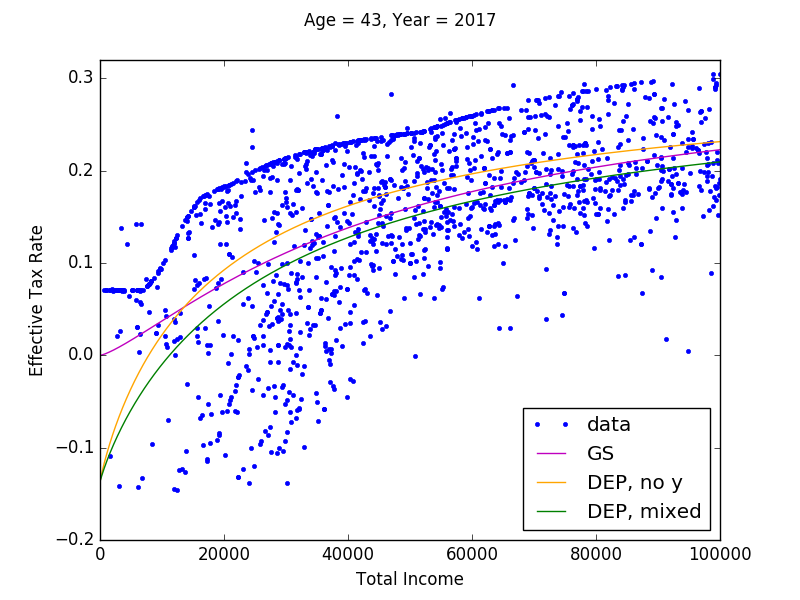
\includegraphics{./images/Compare_ETR_functions.png}}}
  \end{figure}

  Figure \ref{FigTaxCalc3Dtaxrates} shows 3D scatter plots of $ETR$, $MTRx$, and $MTRy$ (and a histogram of the data) with the labor income and capital income, separately, of each age-42 filer in 2017, generated by \taxcalc. This figure presents the main visual evidence for the functional form we use to fit tax functions to these data in Section \ref{SecTaxCalcFuncs}. Figure \ref{FigTaxCalc3Dtaxrates} presents strong evidence that the tax rate---$ETR$, $MTRx$, and $MTRy$---is most accurately modeled as a function of labor income and capital income, separately: $\tau(x,y)$.

  \begin{figure*}[t]\captionsetup{width=6.0in}
    \caption{\label{FigTaxCalc3Dtaxrates}\textbf{Scatter plot of ETR, MTRx, MTRy, and histogram as functions of labor income and capital income from microsimulation model: $t=2017$ and $s=42$ under current law}}
    \fbox{\resizebox{6.0in}{5.0in}{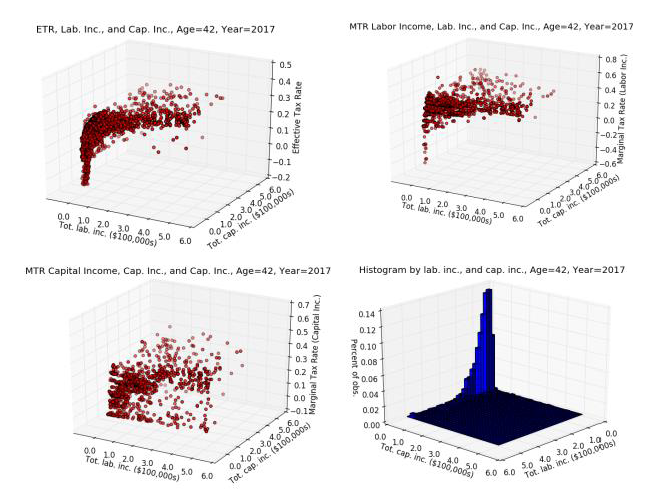
\includegraphics{./images/Age42_2017_scatters.png}}}
    \scriptsize{$^*$Note: Axes in the histogram in the lower-right panel have been switched relative to the other three figures in order to see the distribution more clearly.}
  \end{figure*}


\section{Fitting Tax Functions}\label{SecTaxCalcFuncs}

  In looking at the 2D scatter plot on effective tax rates as a function of total income in Figure \ref{FigTaxCalcETRtotinc} and the 3D scatter plots of $ETR$, $MTRx$, and $MTRy$ in Figure \ref{FigTaxCalc3Dtaxrates}, it is clear that all of these rates exhibit negative exponential or logistic shape. This empirical regularity allows us to make an important and nonrestrictive assumption. We can fit parametric tax rate functions to these data that are constrained to be monotonically increasing in labor income and capital income. This assumption of monotonicity is computationally important as it preserves a convex budget set for each household, which is important for being able to solve many household lifetime problems over a large number of periods.

  \ogindia follows the approach of \citet{DeBackerEtAl:2017} in using the following functional form to estimate tax functions for each age $s=E+1, E+2, ... E+S$ in each time period $t$. Equation \ref{EqTaxCalcTaxFuncForm} is written as a generic tax rate, but we use this same functional form for $ETR$'s, $MTRx$'s, and $MTRy$'s.
  \begin{equation}\label{EqTaxCalcTaxFuncForm}
    \begin{split}
      \tau(x,y) = &\Bigl[\tau(x) + shift_x\Bigr]^\phi\Bigl[\tau(y) + shift_y\Bigr]^{1-\phi} + shift \\
      &\text{where}\quad \tau(x) \equiv (max_x - min_x)\left(\frac{Ax^2 + Bx}{Ax^2 + Bx + 1}\right) + min_x \\
      &\quad\text{and}\quad \tau(y) \equiv (max_y - min_y)\left(\frac{Cy^2 + Dy}{Cy^2 + Dy + 1}\right) + min_y \\
      &\text{where}\quad A,B,C,D,max_x,max_y,shift_x,shift_y > 0 \quad\text{and}\quad\phi\in[0,1] \\
      &\quad\text{and}\quad max_x > min_x \quad\text{and}\quad max_y > min_y
    \end{split}
  \end{equation}
  The parameters values will, in general, differ across the different functions (effective and marginal rate functions) and by age, $s$, and tax year, $t$.  We drop the subscripts for age and year from the above exposition for clarity.

  By assuming each tax function takes the same form, we are breaking the analytical link between the the effective tax rate function and the marginal rate functions.  In particular, one could assume an effective tax rate function and then use the analytical derivative of that to find the marginal tax rate function.  However, we've found it useful to separately estimate the marginal and average rate functions.  One reason is that we want the tax functions to be able to capture policy changes that have differential effects on marginal and average rates.  For example, a change in the standard deduction for tax payers would have a direct effect on their average tax rates.  But it will have secondary effect on marginal rates as well, as some filers will find themselves in different tax brackets after the policy change. These are smaller and second order effects. When tax functions are are fit to the new policy, in this case a lower standard deduction, we want them to be able to represent this differential impact on the marginal and average tax rates. The second reason is related to the first. As the additional flexibility allows us to model specific aspects of tax policy more closely, it also allows us to better fit the parameterized tax functions to the data.

  The key building blocks of the functional form Equation \eqref{EqTaxCalcTaxFuncForm} are the $\tau(x)$ and $\tau(y)$ univariate functions. The ratio of polynomials in the $\tau(x)$ function $\frac{Ax^2 + Bx}{Ax^2 + Bx + 1}$ with positive coefficients $A,B>0$ and positive support for labor income $x>0$ creates a negative-exponential-shaped function that is bounded between 0 and 1, and the curvature is governed by the ratio of quadratic polynomials. The multiplicative scalar term $(max_x-min_x)$ on the ratio of polynomials and the addition of $min_x$ at the end of $\tau(x)$ expands the range of the univariate negative-exponential-shaped function to $\tau(x)\in[min_x, max_x]$. The $\tau(y)$ function is an analogous univariate negative-exponential-shaped function in capital income $y$, such that $\tau(y)\in[min_y,max_y]$.

  The respective $shift_x$ and $shift_y$ parameters in Equation \eqref{EqTaxCalcTaxFuncForm} are analogous to the additive constants in a Stone-Geary utility function. These constants ensure that the two sums $\tau(x) + shift_x$ and $\tau(y) + shift_y$ are both strictly positive. They allow for negative tax rates in the $\tau(\cdot)$ functions despite the requirement that the arguments inside the brackets be strictly positive. The general $shift$ parameter outside of the Cobb-Douglas brackets can then shift the tax rate function so that it can accommodate negative tax rates. The Cobb-Douglas share parameter $\phi\in[0,1]$ controls the shape of the function between the two univariate functions $\tau(x)$ and $\tau(y)$.

  This functional form for tax rates delivers flexible parametric functions that can fit the tax rate data shown in Figure \ref{FigTaxCalc3Dtaxrates} as well as a wide variety of policy reforms. Further, these functional forms are monotonically increasing in both labor income $x$ and capital income $y$. This characteristic of monotonicity in $x$ and $y$ is essential for guaranteeing convex budget sets and thus uniqueness of solutions to the household Euler equations. The assumption of monotonicity does not appear to be a strong one when viewing the the tax rate data shown in Figure \ref{FigTaxCalc3Dtaxrates}. While it does limit the potential tax systems to which one could apply our methodology, tax policies that do not satisfy this assumption would result in non-convex budget sets and thus require non-standard DGE model solutions methods and would not guarantee a unique equilibrium. The 12 parameters of our tax rate functional form from \eqref{EqTaxCalcTaxFuncForm} are summarized in Table \ref{TabTaxCalcTfuncParams}.

  \begin{table}[htbp] \centering \captionsetup{width=5.0in}
  \caption{\label{TabTaxCalcTfuncParams}\textbf{Description of tax rate function $\tau(x,y)$ parameters}}
    \begin{threeparttable}
    \begin{tabular}{>{\footnotesize}c |>{\footnotesize}l }
      \hline\hline
      Symbol & \quad\quad\quad\quad Description  \\
      \hline
      $A$ & Coefficient on squared labor income term $x^2$ in $\tau(x)$ \\
      $B$ & Coefficient on labor income term $x$ in $\tau(x)$ \\
      $C$ & Coefficient on squared capital income term $y^2$ in $\tau(y)$ \\
      $D$ & Coefficient on capital income term $y$ in $\tau(y)$ \\
      $max_x$ & Maximum tax rate on labor income $x$ given $y=0$  \\
      $min_x$ & Minimum tax rate on labor income $x$ given $y=0$ \\
      $max_y$ & Maximum tax rate on capital income $y$ given $x=0$ \\
      $min_y$ & Minimum tax rate on capital income $y$ given $x=0$ \\
      $shift_x$ & shifter $>|min_x|$ ensures that $\tau(x) + shift_x > 0$ despite potentially \\
      & \quad negative values for $\tau(x)$ \\
      $shift_y$ & shifter $>|min_y|$ ensures that $\tau(y) + shift_y > 0$  despite potentially \\
      & \quad negative values for $\tau(y)$ \\
      $shift$ & shifter (can be negative) allows for support of $\tau(x,y)$ to include \\
      & \quad negative tax rates \\
      $\phi$ & Cobb-Douglas share parameter between 0 and 1 \\
      \hline\hline
    \end{tabular}
    % \begin{tablenotes}
    %   \scriptsize{\item[]Note: Maybe put sources here.}
    % \end{tablenotes}
    \end{threeparttable}
  \end{table}

  \begin{figure*}[t]\captionsetup{width=6.0in}
    \caption{\label{FigTaxCalc3DvsPred}\textbf{Estimated tax rate functions of ETR, MTRx, MTRy, and histogram as functions of labor income and capital income from microsimulation model: $t=2017$ and $s=42$ under current law}}
    \fbox{\resizebox{6.0in}{5.0in}{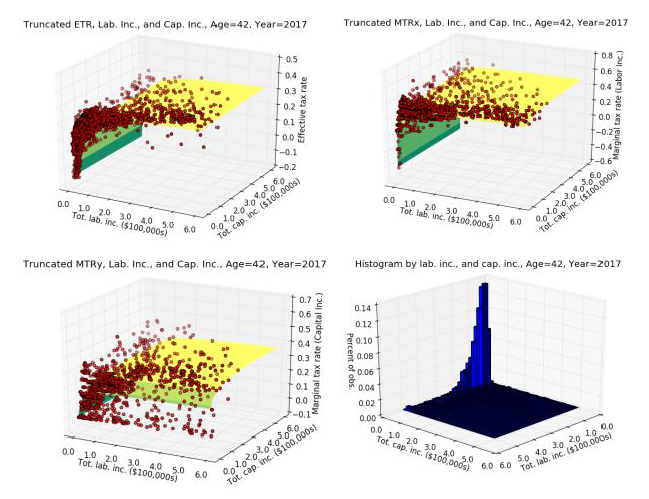
\includegraphics{./images/Age42_2017_vsPred.png}}}
    \scriptsize{$^*$Note: Axes in the histogram in the lower-right panel have been switched relative to the other three figures in order to see the distribution.}
  \end{figure*}

  \begin{table}[htbp] \centering \captionsetup{width=3.0in}
  \caption{\label{TabTaxCalcEst42}\textbf{Estimated baseline current law tax rate function $\tau_{s,t}(x,y)$ parameters for $s=42$, $t=2017$}}
    \begin{threeparttable}
    \begin{tabular}{>{\footnotesize}l |>{\footnotesize}r >{\footnotesize}r >{\footnotesize}r}
    \hline\hline
    Parameter & \multicolumn{1}{c}{\footnotesize{$ETR$}} & \multicolumn{1}{c}{\footnotesize{$MTRx$}} & \multicolumn{1}{c}{\footnotesize{$MTRy$}} \\
    \hline
    $A$ & 6.28E-12 & 3.43E-23 & 4.32E-11 \\
    $B$ & 4.36E-05 & 4.50E-04 & 5.52E-05 \\
    $C$ & 1.04E-23 & 9.81E-12 & 5.62E-12 \\
    $D$ & 7.77E-09 & 5.30E-08 & 3.09E-06 \\
    $max\_{x}$ & 0.80  & 0.71  & 0.44  \\
    $min\_{x}$ & -0.14 & -0.17 & 0.00E+00 \\
    $max\_{y}$ & 0.80  & 0.80  & 0.13 \\
    $min\_{y}$ & -0.15 & -0.42 & 0.00E+00 \\
    $shift\_{x}$ & 0.15  & 0.18  & 4.45E-03 \\
    $shift\_{y}$ & 0.16  & 0.43  & 1.34E-03 \\
    $shift$ & -0.15 & -0.42 & 0.00E+00 \\
    $share$ & 0.84  & 0.96  & 0.86 \\
    \hline
    Obs. (N) & 3,105 & 3,105 & 1,990 \\
    SSE   & 9122.68 & 15041.35 & 7756.54 \\
    \hline\hline
    \end{tabular}
    % \begin{tablenotes}
    %   \scriptsize{\item[]Note: Maybe put sources here.}
    % \end{tablenotes}
    \end{threeparttable}
  \end{table}

  Let $\bm{\theta}_{s,t}=(A,B,C,D,max_x,min_x,max_y,min_y,shift_x,shift_y,shift,\phi)$ be the full vector of 12 parameters of the tax function for a particular type of tax rate, age of filers, and year. We first directly specify $min_x$ as the minimum tax rate and $max_x$ as the maximum tax rate in the data for age-$s$ and period-$t$ individuals for capital income close to 0 ($\$0<y<\$3,000$), and $min_y$ as the minimum tax rate and $max_y$ as the maximum tax rate for labor income close to 0 ($\$0<x<\$3,000$). We then set $shift_x = \min(0,|min_x|)+\ve$ and $shift_y = \min(0,|min_y|)+\ve$ so that the respective arguments in the brackets of \eqref{EqTaxCalcTaxFuncForm} are strictly positive. Then let $shift$ be be the minimum tax rate in the corresponding data minus $\ve$. Let $\bar{\bm{\theta}}_{s,t}=\{min_x,max_x,min_y,max_y,shift_x,shift_y, shift\}$ be the set of parameters we take directly from the data in this way.

  We then estimate five remaining parameters $\tilde{\bm{\theta}}_{s,t}=(A,B,C,D,shift,\phi)$ using the following nonlinear weighted least squares criterion,
  \begin{equation}\label{EqTaxCalcThetaWSSQ}
    \begin{split}
      \bm{\hat{\theta}}_{s,t} = \tilde{\bm{\theta}}_{s,t}:\quad &\min_{\tilde{\bm{\theta}}_{s,t}}\sum_{i=1}^{N} \Bigl[\tau_{i}-\tau_{s,t}\bigl(x_i,y_i|\tilde{\bm{\theta}}_{s,t},\bar{\bm{\theta}}_{s,t}\bigr)\Bigr]^{2} w_i, \\
      &\qquad\text{subject to}\quad A, B, C, D > 0 \quad\text{and}\quad \phi\in[0,1]
    \end{split}
  \end{equation}
  where $\tau_{i}$ is the tax rate for observation $i$ from the microsimulation output, $\tau_{s,t}(x_i,y_i|\tilde{\bm{\theta}}_{s,t},\bar{\bm{\theta}}_{s,t})$ is the predicted tax rate for filing-unit $i$ with $x_{i}$ labor income and $y_{i}$ capital income given parameters $\bm{\theta}_{s,t}$, and $w_{i}$ is the CPS sampling weight of this observation. The number $N$ is the total number of observations from the microsimulation output for age $s$ and year $t$. Figure \ref{FigTaxCalc3DvsPred} shows the typical fit of an estimated tax function $\tau_{s,t}\bigl(x,y|\hat{\bm{\theta}}_{s,t}\bigr)$ to the data. The data in Figure \ref{FigTaxCalc3DvsPred} are the same age $s=42$ and year $t=2017$ as the data Figure \ref{FigTaxCalc3Dtaxrates}.

  The underlying data can limit the number of tax functions that can be estimated. For example, we use the age of the primary filer from the PUF-CPS match to be equivalent to the age of the DGE model household. The DGE model we use allows for individuals up to age 100, however the data contain few primary filers with age above age 80. Because we cannot reliably estimate tax functions for $s>80$, we apply the tax function estimates for 80 year-olds to those with model ages 81 to 100. In the case certain ages below age 80 have too few observations to enable precise estimation of the model parameters, we use a linear interpolation method to find the values for those ages $21\leq s <80$ that cannot be precisely estimated.\footnote{We use two criterion to determine whether the function should be interpolated. First, we require a minimum number of observations of filers of that age and in that tax year. Second, we require that that sum of squared errors meet a predefined threshold.}

  In \ogindia, we estimate the 12-parameter functional form \eqref{EqTaxCalcTaxFuncForm} using weighted nonlinear least squares to fit an effective tax rate function $(\tau^{etr}_{s,t})$, a marginal tax rate of labor income function $(\tau^{mtrx}_{s,t})$, and a marginal tax rate of capital income function $(\tau^{mtry}_{s,t})$ for each age $E+1\leq s\leq E+S$ and each of the first 10 years from the current period.\footnote{We assume that whatever parameters the tax functions have in year 10 persist forever.} That means we have to perform 2,400 estimations of 12 parameters each. Figure \ref{FigTaxCalc3DvsPred} shows the predicted surfaces for $\tau^{etr}_{s=42,t=2017}$, $\tau^{mtrx}_{s=42,t=2017}$, and $\tau^{mtry}_{s=42,t=2017}$ along with the underlying scatter plot data from which those functions were estimated. Table \ref{TabTaxCalcEst42} shows the estimated values of those functional forms.

  The full set of estimated values are calculated in the \href{https://github.com/open-source-economics/OG-USA/blob/master/ogusa/txfunc.py}{\texttt{OG-USA/ogusa/txfunc.py}} module in the \ogindia repository. And the estimated values are stored in the \href{https://github.com/open-source-economics/OG-USA/blob/master/TxFuncEst_baseline.pkl}{\texttt{TxFuncEst\_baseline.pkl}} file.


\section{Factor Transforming Income Units}\label{SecTaxCalcFactor}

  The tax functions $\tau^{etr}_{s,t}$, $\tau^{mtrx}_{s,t}$, and $\tau^{mtry}_{s,t}$ are estimated based on current U.S. tax filer reported incomes in dollars. However, the consumption units of the \ogindia model are not in the same units as the real-world U.S. incomes data. For this reason, we have to transform the income by a $factor$ so that it is in the same units as the income data on which the tax functions were estimated.

  The tax rate functions are each functions of capital income and labor income $\tau(x,y)$. In order to make the tax functions return accurate tax rates associated with the correct levels of income, we multiply the model income $x^m$ and $y^m$ by a $factor$ so that they are in the same units as the real-world U.S. income data $\tau(factor\times x^m, factor\times y^m)$. We define the $factor$ such that average steady-state household total income in the model times the $factor$ equals the U.S. data average total income.
  \begin{equation}\label{EqTaxCalcFactor}
    factor\Biggl[\sum_{s=E+1}^{E+S}\sum_{j=1}^J\lambda_j\bar{\omega}_s\left(\bar{w}e_{j,s}\bar{n}_{j,s} + \bar{r}\bar{b}_{j,s}\right)\Biggr] = \text{Avg. household income in data}
  \end{equation}

  We do not know the steady-state wage, interest rate, household labor supply, and savings \textit{ex ante}. So the income $factor$ is an endogenous variable in the steady-state equilibrium computational solution. We hold the factor constant throughout the nonsteady-state equilibrium solution.


\section{Household Transfers}\label{SecTaxCalcTfers}

  Total transfers to households by the government in a given period $t$ is $TR_t$. The percent of those transfers given to all households of age $s$ and lifetime income group $j$ is $\eta_{j,s}$ such that $\sum_{s=E+1}^{E+S}\sum_{j=1}^J\eta_{j,s,t}=1$. \ogindia currently has the transfer distribution function set to distribute transfers uniformly among the population.
  \begin{equation}\label{EqTaxCalcEtajs}
    \eta_{j,s,t} = \frac{\lambda_j\omega_{s,t}}{\tilde{N}_t} \quad\forall j,t \quad\text{and}\quad E+1\leq s\leq E+S
  \end{equation}
  However, this distribution function $\eta_{j,s,t}$ could also be modified to more accurately reflect the way transfers are distributed in the United States.

  \chapter{Corporate Taxes and B-Tax}\label{Chap_BTax}
    %!TEX root = ../OGUSAdoc.tex

TODO: Have Jason update this chapter to describe how \btax is used to calibrate the values of $\tau^{corp}$ and $\delta^\tau$ from the firm's profit function in \eqref{EqFirmsProfit}.

  \chapter{Unbalanced Government Budget Constraint}\label{Chap_UnbalGBC}
    %!TEX root = ../OGUSAdoc.tex

In \ogindia, the government enters by levying taxes on households, providing transfers to households, levying taxes on firms, spending resources on public goods, and making rule-based adjustments to stabilize the economy in the long-run. It is this last activity that is the focus of this chapter.


\section{Government Tax Revenue}\label{SecUnbalGBCrev}

  We see from the household's budget constraint that taxes $T_{s,t}$ and transfers $TR_{t}$ enter into the household's decision,
  \begin{equation}\tag{\ref{EqHHBC}}
    \begin{split}
      c_{j,s,t} + b_{j,s+1,t+1} &= (1 + r_{t})b_{j,s,t} + w_t e_{j,s} n_{j,s,t} + \zeta_{j,s}\frac{BQ_t}{\lambda_j\omega_{s,t}} + \eta_{j,s,t}\frac{TR_{t}}{\lambda_j\omega_{s,t}} - T_{s,t}  \\
      &\quad\forall j,t\quad\text{and}\quad s\geq E+1 \quad\text{where}\quad b_{j,E+1,t}=0\quad\forall j,t
    \end{split}
  \end{equation}
  where we defined the tax liability function $T_{s,t}$ in \eqref{EqTaxCalcLiabETR} as an effective tax rate times total income and the transfer distribution function $\eta_{j,s,t}$ is uniform across all households as in \eqref{EqTaxCalcEtajs}. And government revenue from the corporate income tax rate $\tau^{corp}$ and the tax on depreciation expensing $\tau^\delta$ enters the firms' profit function.
  \begin{equation}\tag{\ref{EqFirmsProfit}}
    PR_t = (1 - \tau^{corp})\bigl(Y_t - w_t L_t\bigr) - \bigl(r_t + \delta\bigr)K_t + \tau^{corp}\delta^\tau K_t \quad\forall t
  \end{equation}
  We define total government revenue from taxes as the following.
  \begin{equation}\label{EqUnbalGBCgovRev}
    Rev_t = \underbrace{\tau^{corp}\bigl[Y_t - w_t L_t\bigr] - \tau^{corp}\delta^\tau K_t}_{\text{corporate tax revenue}} + \underbrace{\sum_{s=E+1}^{E+S}\sum_{j=1}^J\lambda_j\omega_{s,t}\tau^{etr}_{s,t}\left(x_{j,s,t},y_{j,s,t}\right)\bigl(x_{j,s,t} + y_{j,s,t}\bigr)}_{\text{household tax revenue}} \quad\forall t
  \end{equation}


\section{Government Budget Constraint}\label{SecUnbalGBCbudgConstr}

  Let the level of government debt in period $t$ be given by $D_t$. The government budget constraint requires that government revenue $Rev_t$ plus the budget deficit ($D_{t+1} - D_t$) equal expenditures on interest of the debt, government spending on public goods $G_t$, and total transfer payments to households $TR_t$ every period $t$.
  \begin{equation}\label{EqUnbalGBCbudgConstr}
    D_{t+1} + Rev_t = (1 + r_t)D_t + G_t + TR_t \quad\forall t
  \end{equation}

  We assume that total government transfers to households are a fixed fraction $\alpha_{tr}$ of GDP each period.
  \begin{equation}\label{EqUnbalGBCtfer}
    TR_t = g_{tr,t}\:\alpha_{tr}\: Y_t \quad\forall t
  \end{equation}
  The time dependent multiplier $g_{tr,t}$ in front of the right-hand-side of \eqref{EqUnbalGBCtfer} will equal 1 in most initial periods. It will potentially deviate from 1 in some future periods in order to provide a closure rule that ensures a stable long-run debt-to-GDP ratio. We will discuss the closure rule in Section \ref{SecUnbalGBCcloseRule}.

  We also assume that government spending on public goods is a fixed fraction of GDP each period in the initial periods.
  \begin{equation}\label{EqUnbalGBC_Gt}
    G_t = g_{g,t}\:\alpha_{g}\: Y_t
  \end{equation}
  Similar to transfers $TR_t$, the time dependent multiplier $g_{g,t}$ in front of the right-hand-side of \eqref{EqUnbalGBC_Gt} will equal 1 in most initial periods. It will potentially deviate from 1 in some future periods in order to provide a closure rule that ensures a stable long-run debt-to-GDP ratio. We make this more specific in the next section.


\section{Interest Rate on Government Debt}\label{SecRateWedge}

Despite the model having no aggregate risk, it may be helpful to build in an interest rate differential between the rate of return on private capital and the interest rate on government debt.  Doing so helps to add realism by including a risk premium.  \ogindia allows users to set an exogenous wedge between these two rates.  The interest rate on government debt,

\begin{equation}\label{EqUnbalGBC_rate_wedge}
  r_{gov, t} = (1 - \tau_{d, t})r_{t} - \mu_{d}
\end{equation}

The two parameters, $\tau_{d,t}$ and $\mu_{d,t}$ can be used to allow for a government interest rate that is a percentage hair cut from the market rate or a government interest rate with a constant risk premia.

In the cases where there is a differential ($\tau_{d,t}$ or $\mu_{d,t} \neq 0$), then we need to be careful to specify how the household chooses government debt and private capital in its portfolio of asset holdings.  We make the assumption that under the exogenous interest rate wedge, the household is indifferent between holding its assets as debt and private capital. This amounts to an assumption that these two assets are perfect substitutes given the exogenous wedge in interest rates.  Given the indifference between government debt and private capital at these two interest rates, we assume that the household holds debt and capital in the same ratio that debt and capital are demanded by the government and private firms, respectively. The interest rate on the household portfolio of asset is thus given by:

\begin{equation}\label{EqUnbalGBC_rate_wedge}
  r_{hh,t} = \frac{r_{gov,t}D_{t} + r_{t}K_{t}}{D_{t} + K_{t}}
\end{equation}



\section{Budget Closure Rule}\label{SecUnbalGBCcloseRule}

  If total government transfers to households $TR_t$ and government spending on public goods $G_t$ are both fixed fractions of GDP, one can imagine corporate and household tax structures that cause the debt level of the government to either tend toward infinity or to negative infinity, depending on whether too little revenue or too much revenue is raised, respectively.

  A virtue of dynamic general equilibrium models is that the model must be stationary in order to solve it. That is, no variables can be indefinitely growing as time moves forward. The labor augmenting productivity growth $g_y$ from Chapter \ref{Chap_Firms} and the potential population growth $\tilde{g}_{n,t}$ from Chapter \ref{Chap_Demog} render the model nonstationary. But we show how to stationarize the model against those two sources of growth in Chapter \ref{Chap_Stnrz}. However, even after stationarizing the effects of productivity and population growth, the model could be rendered nonstationary and, therefore, not solvable if government debt were becoming too positive or too negative too quickly.

  The \ogindia model offers three different options for budget closure rules. Each rule uses some combination of changes in government spending on public goods $G_t$ and government transfers to households $TR_t$ to stabilize the debt-to-GDP ratio in the long-run.
  \begin{enumerate}
    \item Change only government spending on public goods $G_t$.
    \item Change only government transfers to households $TR_t$.
    \item Change both government spending $G_t$ and transfers $TR_t$ by the same percentage.
  \end{enumerate}


  \subsection{Change government spending only}\label{SecUnbalGBC_chgGt}

    We specify a closure rule that is automatically implemented after some period $T_{G1}$ to stabilize government debt as a percent of GDP (debt-to-GDP ratio). Let $\alpha_D$ represent the long-run debt-to-GDP ratio at which we want the economy to eventually settle.
    \begin{equation}\label{EqUnbalGBCclosure_Gt}
      \begin{split}
        &G_t = g_{g,t}\:\alpha_{g}\: Y_t \\
        &\text{where}\quad g_{g,t} =
          \begin{cases}
            1 \qquad\qquad\qquad\qquad\qquad\qquad\qquad\:\:\:\,\text{if}\quad t < T_{G1} \\
            \frac{\left[\rho_{d}\alpha_{D}Y_{t} + (1-\rho_{d})D_{t}\right] - (1+r_{t})D_{t} - TR_{t} + Rev_{t}}{\alpha_g Y_t} \quad\text{if}\quad T_{G1}\leq t<T_{G2} \\
            \frac{\alpha_{D}Y_{t} - (1+r_{t})D_{t} - TR_{t} + Rev_{t}}{\alpha_g Y_t} \qquad\qquad\quad\:\:\:\,\text{if}\quad t \geq T_{G2}
          \end{cases} \\
        &\quad\text{and}\quad g_{tr,t} = 1 \quad\forall t
      \end{split}
    \end{equation}
    The first case in \eqref{EqUnbalGBCclosure_Gt} says that government spending $G_t$ will be a fixed fraction $\alpha_g$ of GDP $Y_t$ for every period before $T_{G1}$. The second case specifies that, starting in period $T_{G1}$ and continuing until before period $T_{G2}$, government spending be adjusted to set tomorrow's debt $D_{t+1}$ to be a convex combination between $\alpha_D Y_t$ and the current debt level $D_t$, where $\alpha_D$ is a target debt-to-GDP ratio and $\rho_d\in(0,1]$ is the percent of the way to jump toward the target $\alpha_D Y_t$ from the current debt level $D_t$. The last case specifies that, for every period after $T_{G2}$, government spending $G_t$ is set such that the next-period debt be a fixed target percentage $\alpha_D$ of GDP.


  \subsection{Change government transfers only}\label{SecUnbalGBC_chgTRt}

    If government transfers to households are specified by \eqref{EqUnbalGBCtfer} and the long-run debt-to-GDP ratio can only be stabilized by changing transfers, then the budget closure rule must be the following.
    \begin{equation}\label{EqUnbalGBCclosure_TRt}
      \begin{split}
        &TR_t = g_{tr,t}\:\alpha_{tr}\: Y_t \\
        &\text{where}\quad g_{tr,t} =
          \begin{cases}
            1 \qquad\qquad\qquad\qquad\qquad\qquad\qquad\:\text{if}\quad t < T_{G1} \\
            \frac{\left[\rho_{d}\alpha_{D}Y_{t} + (1-\rho_{d})D_{t}\right] - (1+r_{t})D_{t} - G_{t} + Rev_{t}}{\alpha_{tr} Y_t} \quad\text{if}\quad T_{G1}\leq t<T_{G2} \\
            \frac{\alpha_{D}Y_{t} - (1+r_{t})D_{t} - G_{t} + Rev_{t}}{\alpha_{tr} Y_t} \qquad\qquad\quad\:\:\:\:\text{if}\quad t \geq T_{G2}
          \end{cases} \\
        &\quad\text{and}\quad g_{g,t} = 1 \quad\forall t
      \end{split}
    \end{equation}
    The first case in \eqref{EqUnbalGBCclosure_TRt} says that government transfers $TR_t$ will be a fixed fraction $\alpha_{tr}$ of GDP $Y_t$ for every period before $T_{G1}$. The second case specifies that, starting in period $T_{G1}$ and continuing until before period $T_{G2}$, government transfers be adjusted to set tomorrow's debt $D_{t+1}$ to be a convex combination between $\alpha_D Y_t$ and the current debt level $D_t$. The last case specifies that, for every period after $T_{G2}$, government transfers $TR_t$ are set such that the next-period debt be a fixed target percentage $\alpha_D$ of GDP.


  \subsection{Change both government spending and transfers}\label{SecUnbalGBC_chgGtTRt}

    In some cases, changing only government spending $G_t$ or only government transfers $TR_t$ will not be enough. That is, there exist policies for which a decrease in government spending to zero after period $T_{G1}$ will not stabilize the debt-to-GDP ratio. And negative government spending on public goods does not make sense.\footnote{Negative values for government spending on public goods would mean that revenues are coming into the country from some outside source, which revenues are triggered by government deficits being too high in an arbitrary future period $T_{G2}$.} On the other hand, negative transfers do make sense. Notwithstanding, one might want the added stabilization ability of changing both government spending $G_t$ and transfers $TR_t$ to stabilize the long-run debt-to-GDP ratio.

    In our specific form of this joint option, we assume that the factor by which we scale government spending and transfers is the same $g_{g,t} = g_{tr,t}$ for all $t$. We label this single scaling factor $g_{trg,t}$.
    \begin{equation}\label{EqUnbalGBCclosure_gTRGt}
      g_{trg,t}\equiv g_{g,t} = g_{tr,t} \quad\forall t
    \end{equation}
    If government spending on public goods is specified by \eqref{EqUnbalGBC_Gt} and government transfers to households are specified by \eqref{EqUnbalGBCtfer} and the long-run debt-to-GDP ratio can only be stabilized by changing both spending and transfers, then the budget closure rule must be the following.
    \begin{equation}\label{EqUnbalGBCclosure_TRGt}
      \begin{split}
        &G_t + TR_t = g_{trg,t}\left(\alpha_g + \alpha_{tr}\right)Y_t \quad\Rightarrow\quad G_t = g_{trg,t}\:\alpha_g\: Y_t \quad\text{and}\quad TR_t = g_{trg,t}\:\alpha_{tr}\:Y_t \\
        &\text{where}\quad g_{trg,t} =
          \begin{cases}
            1 \qquad\qquad\qquad\qquad\qquad\qquad\:\:\:\,\text{if}\quad t < T_{G1} \\
            \frac{\left[\rho_{d}\alpha_{D}Y_{t} + (1-\rho_{d})D_{t}\right] - (1+r_{t})D_{t} + Rev_{t}}{\left(\alpha_g + \alpha_{tr}\right)Y_t} \quad\text{if}\quad T_{G1}\leq t<T_{G2} \\
            \frac{\alpha_{D}Y_{t} - (1+r_{t})D_{t} + Rev_{t}}{\left(\alpha_g + \alpha_{tr}\right)Y_t} \qquad\qquad\quad\:\:\:\:\text{if}\quad t \geq T_{G2}
          \end{cases}
      \end{split}
    \end{equation}
    The first case in \eqref{EqUnbalGBCclosure_TRGt} says that government spending and government transfers $Tr_t$ will their respective fixed fractions $\alpha_g$ and $\alpha_{tr}$ of GDP $Y_t$ for every period before $T_{G1}$. The second case specifies that, starting in period $T_{G1}$ and continuing until before period $T_{G2}$, government spending and transfers be adjusted by the same rate to set tomorrow's debt $D_{t+1}$ to be a convex combination between $\alpha_D Y_t$ and the current debt level $D_t$. The last case specifies that, for every period after $T_{G2}$, government spending and transfers are set such that the next-period debt be a fixed target percentage $\alpha_D$ of GDP.

    Each of these budget closure rules \eqref{EqUnbalGBCclosure_Gt}, \eqref{EqUnbalGBCclosure_TRt}, and \eqref{EqUnbalGBCclosure_TRGt} allows the government to run increasing deficits or surpluses in the short run (before period $T_{G1}$). But then the adjustment rule is implemented gradually beginning in period $t=T_{G1}$ to return the debt-to-GDP ratio back to its long-run target of $\alpha_D$. Then the rule is implemented exactly in period $T_{G2}$ by adjusting some combination of government spending $G_t$ and transfers $TR_t$ to set the debt $D_{t+1}$ such that it is exactly $\alpha_D$ proportion of GDP $Y_t$.


\section{Some Caveats and Alternatives}\label{SecUnbalGBCcaveat}

  \ogindia adjusts some combination of government spending $G_t$ and government transfers $TR_t$ as its closure rule instrument because of its simplicity and lack of distortionary effects. Since government spending does not enter into the household's utility function, its level does not affect the solution of the household problem. In contrast, government transfers do appear in the household budget constraint. However, household decisions do not individually affect the amount of transfers, thereby rendering government transfers as exogenous from the household's perspective. As an alternative, one could choose to adjust taxes to close the budget (or a combination of all of the government fiscal policy levers).

  There is no guarantee that any of our stated closure rules \eqref{EqUnbalGBCclosure_Gt}, \eqref{EqUnbalGBCclosure_TRt}, or \eqref{EqUnbalGBCclosure_TRGt} is sufficient to stabilize the debt-to-GDP ratio in the long run. For large and growing deficits, the convex combination parameter $\rho_d$ might be too gradual, or the budget closure initial period $T_{G1}$ might be too far in the future, or the target debt-to-GDP ratio $\alpha_D$ might be too high. The existence of any of these problems might be manifest in the steady state computation stage. However, it is possible for the steady-state to exist, but for the time path to never reach it. These problems can be avoided by choosing conservative values for $T_{G1}$, $\rho_d$, and $\alpha_D$ that close the budget quickly.

  And finally, in closure rules \eqref{EqUnbalGBCclosure_Gt} and \eqref{EqUnbalGBCclosure_TRGt} in which government spending is used to stabilize the long-run budget, it is also possible that government spending is forced to be less than zero to make this happen. This would be the case if tax revenues bring in less than is needed to financed transfers and interest payments on the national debt. None of the equations we've specified above preclude that result, but it does raise conceptual difficulties. Namely, what does it mean for government spending to be negative? Is the government selling off pubic assets? We caution those using this budget closure rule to consider carefully how the budget is closed in the long run given their parameterization. We also note that such difficulties present themselves across all budget closure rules when analyzing tax or spending proposals that induce structural budget deficits. In particular, one probably needs a different closure instrument if government spending must be negative in the steady-state to hit your long-term debt-to-GDP target.


\part{Market clearing and Stationarization}\label{PartMCstat}
  \chapter{Market Clearing}\label{Chap_MarkClr}
    %!TEX root = ../OGUSAdoc.tex

Three markets must clear in \ogindia---the labor market, the capital market, and the goods market. By Walras' Law, we only need to use two of those market clearing conditions because the third one is redundant. In the model, we choose to use the labor market clearing condition and the capital market clearing condition, and to ignore the goods market clearing condition. But we present all three market clearing conditions here. Further, the redundant goods market clearing condition---sometimes referred to as the resource constraint---makes for a nice check on the solution method to see if everything worked.

We also characterize here the law of motion for total bequests $BQ_t$. Although it is not technically a market clearing condition, one could think of the bequests law of motion as the bequests market clearing condition.

\section{Market Clearing Conditions}\label{SecMarkClrMktClr}

  Labor market clearing \eqref{EqMarkClrLab} requires that aggregate labor demand $L_t$ measured in efficiency units equal the sum of household efficiency labor supplied $e_{j,s}n_{j,s,t}$.
  \begin{equation}\label{EqMarkClrLab}
    L_t = \sum_{s=E+1}^{E+S}\sum_{j=1}^{J} \omega_{s,t}\lambda_j e_{j,s}n_{j,s,t} \quad \forall t
  \end{equation}
  Capital market clearing \eqref{EqMarkClrCap} requires that aggregate capital demand from firms $K_t$ and from the government $D_t$ equal the sum of capital savings and investment by households $b_{j,s,t}$.
  \begin{equation}\label{EqMarkClrCap}
    K_t + D_t = \sum_{s=E+2}^{E+S+1}\sum_{j=1}^{J}\Bigl(\omega_{s-1,t-1}\lambda_j b_{j,s,t} + i_s\omega_{s,t-1}\lambda_j b_{j,s,t}\Bigr) \quad \forall t
  \end{equation}
  Note that the capital demand side of the capital market clearing equation \eqref{EqMarkClrCap} includes both capital demand by firms $K_t$ and capital demand by government $D_t$. It is here that we can see the potential of government deficits to crowd out investment.

  Aggregate consumption $C_t$ is defined as the sum of all household consumptions, and aggregate investment is defined by the resource constraint $Y_t = C_t + I_t + G_t$ as shown in \eqref{EqMarkClrGoods}.
  \begin{equation}\label{EqMarkClrGoods}
    \begin{split}
      Y_t &= C_t + K_{t+1} - \biggl(\sum_{s=E+2}^{E+S+1}\sum_{j=1}^{J}i_s\omega_{s,t}\lambda_j b_{j,s,t+1}\biggr) - (1-\delta)K_t + G_t \quad\forall t \\
      &\quad\text{where}\quad C_t \equiv \sum_{s=E+1}^{E+S}\sum_{j=1}^{J}\omega_{s,t}\lambda_j c_{j,s,t}
    \end{split}
  \end{equation}

  Note that the extra terms with the immigration rate $i_s$ in the capital market clearing equation \eqref{EqMarkClrCap} and the resource constraint \eqref{EqMarkClrGoods} accounts for the assumption that age-$s$ immigrants in period $t$ bring with them (or take with them in the case of out-migration) the same amount of capital as their domestic counterparts of the same age. Note also that the term in parentheses with immigration rates $i_s$ in the sum acts is equivalent to a net exports term in the standard equation $Y=C+I+G+NX$. That is, if immigration rates are positive, then immigrants are bringing capital into the country and the term in parentheses has a negative sign in front of it. Negative exports are imports.


\section{Total Bequests Law of Motion}\label{SecMarkClrBQ}

  Total bequests $BQ_t$ are the collection of savings of household from the previous period who died at the end of the period. These savings are augmented by the interest rate because they are returned after being invested in the production process.
  \begin{equation}\label{EqMarkClrBQ}
    BQ_{t} = (1+r_{t})\left(\sum_{s=E+2}^{E+S+1}\sum_{j=1}^J\rho_{s-1}\lambda_j\omega_{s-1,t-1}b_{j,s,t}\right) \quad\forall t
  \end{equation}
  Because the form of the period utility function in \eqref{EqHHPerUtil} ensures that $b_{j,s,t}>0$ for all $j$, $s$, and $t$, total bequests will always be positive $BQ_{j,t}>0$ for all $j$ and $t$.

  \chapter{Stationarization}\label{Chap_Stnrz}
    %!TEX root = ../OGUSAdoc.tex

The previous chapters derive all the equations necessary to solve for the steady-state and nonsteady-state equilibria of this model. However, because labor productivity is growing at rate $g_y$ as can be seen in the firms' production function \eqref{EqFirmsCESprodfun} and the population is growing at rate $\tilde{g}_{n,t}$ as defined in \eqref{EqPopGrowthTil}, the model is not stationary. Different endogenous variables of the model are growing at different rates. We have already specified three potential budget closure rules \eqref{EqUnbalGBCclosure_Gt}, \eqref{EqUnbalGBCclosure_TRt}, and \eqref{EqUnbalGBCclosure_TRGt} using some combination of government spending $G_t$ and transfers $TR_t$ that stationarize the debt-to-GDP ratio.

Table \ref{TabStnrzStatVars} lists the definitions of stationary versions of these endogenous variables. Variables with a ``$\:\,\hat{}\,\:$'' signify stationary variables. The first column of variables are growing at the productivity growth rate $g_y$. These variables are most closely associated with individual variables. The second column of variables are growing at the population growth rate $\tilde{g}_{n,t}$. These variables are most closely associated with population values. The third column of variables are growing at both the productivity growth rate $g_y$ and the population growth rate $\tilde{g}_{n,t}$. These variables are most closely associated with aggregate variables. The last column shows that the interest rate $r_t$ and household labor supply $n_{j,s,t}$ are already stationary.

\begin{table}[htbp] \centering \captionsetup{width=3.5in}
\caption{\label{TabStnrzStatVars}\textbf{Stationary variable definitions}}
  \begin{threeparttable}
  \begin{tabular}{>{\small}c >{\small}c >{\small}c |>{\small}c}
    \hline\hline
    \multicolumn{3}{c}{Sources of growth} & Not \\
    & & & \\[-4mm]
    $e^{g_y t}$ & $\tilde{N}_t$ & $e^{g_y t}\tilde{N}_t$ & growing\tnote{a} \\
    \hline
    & & \\[-4mm]
    $\hat{c}_{j,s,t}\equiv\frac{c_{j,s,t}}{e^{g_y t}}$ & $\hat{\omega}_{s,t}\equiv\frac{\omega_{s,t}}{\tilde{N}_t}$ & $\hat{Y}_t\equiv\frac{Y_t}{e^{g_y t}\tilde{N}_t}$ & $n_{j,s,t}$ \\[2mm]
    $\hat{b}_{j,s,t}\equiv\frac{b_{j,s,t}}{e^{g_y t}}$ & $\hat{L}_t\equiv\frac{L_t}{\tilde{N}_t}$ & $\hat{K}_t\equiv\frac{K_t}{e^{g_y t}\tilde{N}_t}$ & $r_t$ \\[2mm]
    $\hat{w}_t\equiv\frac{w_t}{e^{g_y t}}$ &  & $\hat{BQ}_{j,t}\equiv\frac{BQ_{j,t}}{e^{g_y t}\tilde{N}_t}$ &  \\[2mm]
    $\hat{y}_{j,s,t}\equiv\frac{y_{j,s,t}}{e^{g_y t}}$ &  & $\hat{C}_t\equiv \frac{C_t}{e^{g_y t}\tilde{N}_t}$  &  \\[2mm]
    $\hat{T}_{s,t}\equiv\frac{T_{j,s,t}}{e^{g_y t}}$ &  & $\hat{TR}_t\equiv\frac{TR_t}{e^{g_y t}\tilde{N}_t}$ &  \\[2mm]
    \hline\hline
  \end{tabular}
  \begin{tablenotes}
    \scriptsize{\item[a]The interest rate $r_t$ in \eqref{EqFirmFOC_K} is already stationary because $Y_t$ and $K_t$ grow at the same rate. Household labor supply $n_{j,s,t}\in[0,\tilde{l}]$ is stationary.}
  \end{tablenotes}
  \end{threeparttable}
\end{table}

The usual definition of equilibrium would be allocations and prices such that households optimize \eqref{EqHHeul_n}, \eqref{EqHHeul_b}, and \eqref{EqHHeul_bS}, firms optimize \eqref{EqFirmFOC_L} and \eqref{EqFirmFOC_K}, and markets clear \eqref{EqMarkClrLab} and \eqref{EqMarkClrCap}, and \eqref{EqMarkClrBQ}. In this chapter, we show how to stationarize each of these characterizing equations so that we can use our fixed point methods described in Sections \ref{SecEqlbSSsoln} and \ref{SecEqlbNSSsoln} to solve for the equilibria in Definitions \ref{DefSSEql} and \ref{DefNSSEql}.


\section{Stationarized Household Equations}\label{SecStnrzHH}

  The stationary version of the household budget constraint \eqref{EqHHBC} is found by dividing both sides of the equation by $e^{g_y t}$. For the savings term $b_{j,s+1,t+1}$, we must multiply and divide by $e^{g_y(t+1)}$, which leaves an $e^{g_y} = \frac{e^{g_y(t+1)}}{e^{g_y t}}$ in front of the stationarized variable.
  \begin{equation}\label{EqStnrzHHBCstat}
    \begin{split}
      \hat{c}_{j,s,t} + e^{g_y}\hat{b}_{j,s+1,t+1} &= (1 + r_{t})\hat{b}_{j,s,t} + \hat{w}_t e_{j,s} n_{j,s,t} + \zeta_{j,s}\frac{\hat{BQ}_t}{\lambda_j\hat{\omega}_{s,t}} + \eta_{j,s,t}\frac{\hat{TR}_{t}}{\lambda_j\hat{\omega}_{s,t}} - \hat{T}_{s,t}  \\
      &\quad\forall j,t\quad\text{and}\quad s\geq E+1 \quad\text{where}\quad b_{j,E+1,t}=0\quad\forall j,t
    \end{split}
  \end{equation}
  Because total bequests $BQ_t$ and total government transfers $TR_t$ grow at both the labor productivity growth rate and the population growth rate, we have to multiply and divide each of those terms by the economically relevant population $\tilde{N}_t$. This stationarizes total bequests $\hat{BQ}_t$, total transfers $\hat{TR}_t$, and the respective population level in the denominator $\hat{\omega}_{s,t}$.

  We stationarize the Euler equations for labor supply \eqref{EqHHeul_n} by dividing both sides by $e^{g_y(1-\sigma)}$. On the left-hand-side, $e^{g_y}$ stationarizes the wage $\hat{w}_t$ and $e^{-\sigma g_y}$ goes inside the parentheses and stationarizes consumption $\hat{c}_{j,s,t}$. On the right-and-side, the $e^{g_y(1-\sigma)}$ terms cancel out.
  \begin{equation}\label{EqStnrzHHeul_n}
    \begin{split}
      &\hat{w}_t e_{j,s}\bigl(1 - \tau^{mtrx}_{s,t}\bigr)(\hat{c}_{j,s,t})^{-\sigma} = \chi^n_{s}\biggl(\frac{b}{\tilde{l}}\biggr)\biggl(\frac{n_{j,s,t}}{\tilde{l}}\biggr)^{\upsilon-1}\Biggl[1 - \biggl(\frac{n_{j,s,t}}{\tilde{l}}\biggr)^\upsilon\Biggr]^{\frac{1-\upsilon}{\upsilon}} \\
      &\qquad\qquad\qquad\qquad\qquad\qquad\qquad\qquad\forall j,t, \quad\text{and}\quad E+1\leq s\leq E+S \\
    \end{split}
  \end{equation}

  We stationarize the Euler equations for savings \eqref{EqHHeul_b} and \eqref{EqHHeul_bS} by dividing both sides of the respective equations by $e^{-\sigma g_y t}$. On the right-hand-side of the equation, we then need to multiply and divide both terms by $e^{-\sigma g_y(t+1)}$, which leaves a multiplicative coefficient $e^{-\sigma g_y}$.
  \begin{equation}\label{EqStnrzHHeul_b}
    \begin{split}
      &(\hat{c}_{j,s,t})^{-\sigma} = e^{-\sigma g_y}\biggl[\chi^b_j\rho_s(\hat{b}_{j,s+1,t+1})^{-\sigma} + \beta\bigl(1 - \rho_s\bigr)\Bigl(1 + r_{t+1}\bigl[1 - \tau^{mtry}_{s+1,t+1}\bigr]\Bigr)(\hat{c}_{j,s+1,t+1})^{-\sigma}\biggr] \\
      &\qquad\qquad\qquad\qquad\qquad\qquad\qquad\qquad\forall j,t, \quad\text{and}\quad E+1\leq s\leq E+S-1 \\
    \end{split}
  \end{equation}

  \begin{equation}\label{EqStnrzHHeul_bS}
    (\hat{c}_{j,E+S,t})^{-\sigma} = e^{-\sigma g_y}\chi^b_j(\hat{b}_{j,E+S+1,t+1})^{-\sigma} \quad\forall j,t \quad\text{and}\quad s = E+S
  \end{equation}


\section{Stationarized Firms Equations}\label{SecStnrzFirms}

  The nonstationary production function \eqref{EqFirmsCESprodfun} can be stationarized by dividing both sides by $e^{g_y t}\tilde{N}$. This stationarizes output $\hat{Y}_t$ on the left-hand-side. Because the general CES production function is homogeneous of degree 1, $F(xK,xL) = xF(K,L)$, which means the right-hand-side of the production function is stationarized by dividing by $e^{g_y t}\tilde{N}_t$.
  \begin{equation}\label{EqStnrzCESprodfun}
    \hat{Y}_t = F(\hat{K}_t, \hat{L}_t) \equiv Z_t\biggl[(\gamma)^\frac{1}{\ve}(\hat{K}_t)^\frac{\ve-1}{\ve} + (1-\gamma)^\frac{1}{\ve}(\hat{L}_t)^\frac{\ve-1}{\ve}\biggr]^\frac{\ve}{\ve-1} \quad\forall t
  \end{equation}
  Notice that the growth term multiplied by the labor input drops out in this stationarized version of the production function. We stationarize the nonstationary profit function \eqref{EqFirmsProfit} in the same way, by dividing both sides by $e^{g_y t}\tilde{N}_t$.
  \begin{equation}\label{EqStnrzProfit}
    \hat{PR}_t = (1 - \tau^{corp})\Bigl[F(\hat{K}_t,\hat{L}_t) - \hat{w}_t \hat{L}_t\Bigr] - \bigl(r_t + \delta\bigr)\hat{K}_t + \tau^{corp}\delta^\tau \hat{K}_t \quad\forall t
  \end{equation}

  The firms' first order equation for labor demand \eqref{EqFirmFOC_L} is stationarized by dividing both sides by $e^{g_y t}$. This stationarizes the wage $\hat{w}_t$ on the left-hand-side and cancels out the $e^{g_y t}$ term in front of the right-hand-side. To complete the stationarization, we multiply and divide the $\frac{Y_t}{e^{g_y t}L_t}$ term on the right-hand-side by $\tilde{N}_t$.
  \begin{equation}\label{EqStnrzFOC_L}
    \hat{w}_t = (Z_t)^\frac{\ve-1}{\ve}\left[(1-\gamma)\frac{\hat{Y}_t}{\hat{L}_t}\right]^\frac{1}{\ve} \quad\forall t
  \end{equation}

  It can be seen from the firms' first order equation for capital demand \eqref{EqFirmFOC_K} that the interest rate is already stationary. If we multiply and divide the $\frac{Y_t}{K_t}$ term on the right-hand-side by $e^{t_y t}\tilde{N}_t$, those two aggregate variables become stationary. In other words, $Y_t$ and $K_t$ grow at the same rate and $\frac{Y_t}{K_t} = \frac{\hat{Y}_t}{\hat{K}_t}$.
  \begin{equation}\tag{\ref{EqFirmFOC_K}}
    \begin{split}
      r_t &= (1 - \tau^{corp})(Z_t)^\frac{\ve-1}{\ve}\left[\gamma\frac{\hat{Y}_t}{\hat{K}_t}\right]^\frac{1}{\ve} - \delta + \tau^{corp}\delta^\tau \quad\forall t \\
      &= (1 - \tau^{corp})(Z_t)^\frac{\ve-1}{\ve}\left[\gamma\frac{Y_t}{K_t}\right]^\frac{1}{\ve} - \delta + \tau^{corp}\delta^\tau \quad\forall t
    \end{split}
  \end{equation}


\section{Stationarized Government Equations}\label{SecStnrzGovt}

  Each of the tax rate functions $\tau^{etr}_{s,t}$, $\tau^{mtrx}_{s,t}$, and $\tau^{mtry}_{s,t}$ is stationary. The total tax liability function $T_{s,t}$ is growing at the rate of labor productivity growth $g_y$ This can be see by looking at the decomposition of the total tax liability function into the effective tax rate times total income \eqref{EqTaxCalcLiabETR}. The effective tax rate function is stationary, and household income is growing at rate $g_y$. So household total tax liability is stationarized by dividing both sides of the equation by $e^{g_y t}$.
  \begin{equation}\label{EqStnrzLiabETR}
    \begin{split}
      \hat{T}_{s,t} &= \tau^{etr}_{s,t}(\hat{x}_{j,s,t}, \hat{y}_{j,s,t})\left(\hat{x}_{j,s,t} + \hat{y}_{j,s,t}\right) \qquad\qquad\qquad\quad\:\:\forall t \quad\text{and}\quad E+1\leq s\leq E+S \\
      &= \tau^{etr}_{s,t}(\hat{w}_t e_{j,s}n_{j,s,t}, r_t\hat{b}_{j,s,t})\left(\hat{w}_t e_{j,s}n_{j,s,t} + r_t\hat{b}_{j,s,t}\right) \quad\forall t \quad\text{and}\quad E+1\leq s\leq E+S
    \end{split}
  \end{equation}

  We can stationarize the simple expressions for total government spending on public goods $G_t$ in \eqref{EqUnbalGBC_Gt} and on household transfers $TR_t$ in \eqref{EqUnbalGBCtfer} by dividing both sides by $e^{g_y t}\tilde{N}_t$,
  \begin{equation}\label{EqStnrz_Gt}
    \hat{G}_t = g_{g,t}\:\alpha_{g}\:\hat{Y}_t \quad\forall t
  \end{equation}
  \begin{equation}\label{EqStnrzTfer}
    \hat{TR}_t = g_{tr,t}\:\alpha_{tr}\:\hat{Y}_t \quad\forall t
  \end{equation}
  where the time varying multipliers $g_{g,t}$ and $g_{tr,t}$, respectively, are defined in \eqref{EqStnrzClosureRule_Gt} and \eqref{EqStnrzClosureRule_TRt} below. These multipliers $g_{g,t}$ and $g_{tr,t}$ do not have a ``$\:\,\hat{}\,\:$'' on them because their specifications \eqref{EqUnbalGBCclosure_Gt} and \eqref{EqUnbalGBCclosure_TRt} that are functions of nonstationary variables are equivalent to \eqref{EqStnrzClosureRule_Gt} and \eqref{EqStnrzClosureRule_TRt} specified in stationary variables.

  We can stationarize the expression for total government revenue $Rev_t$ in \eqref{EqUnbalGBCgovRev} by dividing both sides of the equation by $e^{g_y t}\tilde{N}_t$.
  \begin{equation}\label{EqStnrzGovRev}
    \hat{Rev}_t = \underbrace{\tau^{corp}\bigl[\hat{Y}_t - \hat{w}_t\hat{L}_t\bigr] - \tau^{corp}\delta^\tau \hat{K}_t}_{\text{corporate tax revenue}} + \underbrace{\sum_{s=E+1}^{E+S}\sum_{j=1}^J\lambda_j\hat{\omega}_{s,t}\tau^{etr}_{s,t}\left(\hat{x}_{j,s,t},\hat{y}_{j,s,t}\right)\bigl(\hat{x}_{j,s,t} + \hat{y}_{j,s,t}\bigr)}_{\text{household tax revenue}} \quad\forall t
  \end{equation}
  Every term in the government budget constraint \eqref{EqUnbalGBCbudgConstr} is growing at both the productivity growth rate and the population growth rate, so we stationarize it by dividing both sides by $e^{g_y t}\tilde{N}_t$. We also have to multiply and divide the next period debt term $D_{t+1}$ by $e^{g_y(t+1)}\tilde{N}_{t+1}$, leaving the term $e^{g_y}(1 + \tilde{g}_{n,t+1})$.
  \begin{equation}\label{EqStnrzGovBC}
    e^{g_y}\left(1 + \tilde{g}_{n,t+1}\right)\hat{D}_{t+1} + \hat{Rev}_t = (1 + r_t)\hat{D}_t + \hat{G}_t + \hat{TR}_t \quad\forall t
  \end{equation}

  The three potential budget closure rules \eqref{EqUnbalGBCclosure_Gt}, \eqref{EqUnbalGBCclosure_TRt}, and \eqref{EqUnbalGBCclosure_TRGt} are the last government equations to stationarize. In each of the cases, we simply divide both sides by $e^{g_y t}\tilde{N}_t$.
  \begin{equation}\label{EqStnrzClosureRule_Gt}
      \begin{split}
        &\hat{G}_t = g_{g,t}\:\alpha_{g}\: \hat{Y}_t \\
        &\text{where}\quad g_{g,t} =
          \begin{cases}
            1 \qquad\qquad\qquad\qquad\qquad\qquad\qquad\qquad\qquad\quad\:\:\text{if}\quad t < T_{G1} \\
            \frac{e^{g_y}\left(1 + \tilde{g}_{n,t+1}\right)\left[\rho_{d}\alpha_{D}\hat{Y}_{t} + (1-\rho_{d})\hat{D}_{t}\right] - (1+r_{t})\hat{D}_{t} - \hat{TR}_{t} + \hat{Rev}_{t}}{\alpha_g \hat{Y}_t} \quad\text{if}\quad T_{G1}\leq t<T_{G2} \\
            \frac{e^{g_y}\left(1 + \tilde{g}_{n,t+1}\right)\alpha_{D}\hat{Y}_{t} - (1+r_{t})\hat{D}_{t} - \hat{TR}_{t} + \hat{Rev}_{t}}{\alpha_g \hat{Y}_t} \qquad\qquad\qquad\text{if}\quad t \geq T_{G2}
          \end{cases} \\
        &\quad\text{and}\quad g_{tr,t} = 1 \quad\forall t
      \end{split}
    \end{equation}
  or
  \begin{equation}\label{EqStnrzClosureRule_TRt}
    \begin{split}
        &\hat{TR}_t = g_{tr,t}\:\alpha_{tr}\: \hat{Y}_t \\
        &\text{where}\quad g_{tr,t} =
          \begin{cases}
            1 \qquad\qquad\qquad\qquad\qquad\qquad\qquad\qquad\qquad\quad\text{if}\quad t < T_{G1} \\
            \frac{e^{g_y}\left(1 + \tilde{g}_{n,t+1}\right)\left[\rho_{d}\alpha_{D}\hat{Y}_{t} + (1-\rho_{d})\hat{D}_{t}\right] - (1+r_{t})\hat{D}_{t} - \hat{G}_{t} + \hat{Rev}_{t}}{\alpha_{tr} \hat{Y}_t} \quad\text{if}\quad T_{G1}\leq t<T_{G2} \\
            \frac{e^{g_y}\left(1 + \tilde{g}_{n,t+1}\right)\alpha_{D}\hat{Y}_{t} - (1+r_{t})\hat{D}_{t} - \hat{G}_{t} + \hat{Rev}_{t}}{\alpha_{tr} \hat{Y}_t} \qquad\qquad\qquad\text{if}\quad t \geq T_{G2}
          \end{cases} \\
      &\quad\text{and}\quad g_{g,t} = 1 \quad\forall t
      \end{split}
  \end{equation}
  or
  \begin{equation}\label{EqStnrzClosureRule_TRGt}
      \begin{split}
        &\hat{G}_t + \hat{TR}_t = g_{trg,t}\left(\alpha_g + \alpha_{tr}\right)\hat{Y}_t \quad\Rightarrow\quad \hat{G}_t = g_{trg,t}\:\alpha_g\:\hat{Y}_t \quad\text{and}\quad \hat{TR}_t = g_{trg,t}\:\alpha_{tr}\:\hat{Y}_t \\
        &\text{where}\quad g_{trg,t} =
          \begin{cases}
            1 \qquad\qquad\qquad\qquad\qquad\qquad\qquad\qquad\quad\:\:\,\text{if}\quad t < T_{G1} \\
            \frac{e^{g_y}\left(1 + \tilde{g}_{n,t+1}\right)\left[\rho_{d}\alpha_{D}\hat{Y}_{t} + (1-\rho_{d})\hat{D}_{t}\right] - (1+r_{t})\hat{D}_{t} + \hat{Rev}_{t}}{\left(\alpha_g + \alpha_{tr}\right)\hat{Y}_t} \quad\text{if}\quad T_{G1}\leq t<T_{G2} \\
            \frac{e^{g_y}\left(1 + \tilde{g}_{n,t+1}\right)\alpha_{D}\hat{Y}_{t} - (1+r_{t})\hat{D}_{t} + \hat{Rev}_{t}}{\left(\alpha_g + \alpha_{tr}\right)\hat{Y}_t} \qquad\qquad\quad\:\:\:\:\,\text{if}\quad t \geq T_{G2}
          \end{cases}
      \end{split}
    \end{equation}


\section{Stationarized Market Clearing Equations}\label{SecStnrzMC}

  The labor market clearing equation \eqref{EqMarkClrLab} is stationarized by dividing both sides by $\tilde{N}_t$.
  \begin{equation}\label{EqStnrzMarkClrLab}
    \hat{L}_t = \sum_{s=E+1}^{E+S}\sum_{j=1}^{J} \hat{\omega}_{s,t}\lambda_j e_{j,s}n_{j,s,t} \quad \forall t
  \end{equation}
  The capital market clearing equation \eqref{EqMarkClrCap} is stationarized by dividing both sides by $e^{g_y t}\tilde{N}_t$. Because the right-hand-side has population levels from the previous period $\omega_{s,t-1}$, we have to multiply and divide both terms inside the parentheses by $\tilde{N}_{t-1}$ which leaves us with the term in front of $\frac{1}{1+\tilde{g}_{n,t}}$.
  \begin{equation}\label{EqStnrzMarkClrCap}
    \hat{K}_t + \hat{D}_t = \frac{1}{1 + \tilde{g}_{n,t}}\sum_{s=E+2}^{E+S+1}\sum_{j=1}^{J}\Bigl(\hat{\omega}_{s-1,t-1}\lambda_j \hat{b}_{j,s,t} + i_s\hat{\omega}_{s,t-1}\lambda_j \hat{b}_{j,s,t}\Bigr) \quad \forall t
  \end{equation}

  We stationarize the goods market clearing \eqref{EqMarkClrGoods} condition by dividing both sides by $e^{g_y t}\tilde{N}_t$. On the right-hand-side, we must multiply and divide the $K_{t+1}$ term by $e^{g_y(t+1)}\tilde{N}_{t+1}$ leaving the coefficient $e^{g_y}(1+\tilde{g}_{n,t+1})$. And the term that subtracts the sum of imports of next period's immigrant savings we must multiply and divide by $e^{g_(t+1)}$, which leaves the term $e^{g_y}$.
  \begin{equation}\label{EqStnrzMarkClrGoods}
    \begin{split}
      \hat{Y}_t &= \hat{C}_t + e^{g_y}(1 + \tilde{g}_{n,t+1})\hat{K}_{t+1} - e^{g_y}\biggl(\sum_{s=E+2}^{E+S+1}\sum_{j=1}^{J}i_s\hat{\omega}_{s,t}\lambda_j \hat{b}_{j,s,t+1}\biggr) - (1-\delta)\hat{K}_t + \hat{G}_t \quad\forall t \\
      &\quad\text{where}\quad \hat{C}_t \equiv \sum_{s=E+1}^{E+S}\sum_{j=1}^{J}\hat{\omega}_{s,t}\lambda_j\hat{c}_{j,s,t}
    \end{split}
  \end{equation}

  We stationarize the law of motion for total bequests $BQ_t$ in \eqref{EqMarkClrBQ} by dividing both sides by $e^{g_y t}\tilde{N}_t$. Because the population levels in the summation are from period $t-1$, we must multiply and divide the summed term by $\tilde{N}_{t-1}$ leaving the term in the denominator of $1+\tilde{g}_{n,t}$.
  \begin{equation}\label{EqStnrzMarkClrBQ}
    \hat{BQ}_{t} = \left(\frac{1+r_{t}}{1 + \tilde{g}_{n,t}}\right)\left(\sum_{s=E+2}^{E+S+1}\sum_{j=1}^J\rho_{s-1}\lambda_j\hat{\omega}_{s-1,t-1}\hat{b}_{j,s,t}\right) \quad\forall t
  \end{equation}


\part{Equilibrium Definitions and Solution Methods}\label{PartEqlbm}
  \chapter{Stationary Steady-state Equilibrium}\label{Chap_SSeqlb}
    %!TEX root = ../OGUSAdoc.tex

In this chapter, we define the stationary steady-state equilibrium of the \ogindia model. Chapters \ref{Chap_Demog} through \ref{Chap_MarkClr} derive the equations that characterize the equilibrium of the model. However, we cannot solve for any equilibrium of the model in the presence of nonstationarity in the variables. Nonstationarity in \ogindia comes from productivity growth $g_y$ in the production function \eqref{EqFirmsCESprodfun}, population growth $\tilde{g}_{n,t}$ as described in Chapter \ref{Chap_Demog}, and the potential for unbounded growth in government debt as described in Chapter \ref{Chap_UnbalGBC}.

We implemented an automatic government budget closure rule using government spending $G_t$ as the instrument that stabilizes the debt-to-GDP ratio at a long-term rate in \eqref{EqUnbalGBCclosure}. And we showed in Chapter \ref{Chap_Stnrz} how to stationarize all the other characterizing equations.


\section{Stationary Steady-State Equilibrium Definition}\label{SecEqlbSSdef}

  With the stationarized model, we can now define the stationary steady-state equilibrium. This equilibrium will be long-run values of the endogenous variables that are constant over time. In a perfect foresight model, the steady-state equilibrium is the state of the economy at which the model settles after a finite amount of time, regardless of the initial condition of the model. Once the model arrives at the steady-state, it stays there indefinitely unless it receives some type of shock or stimulus.

  These stationary values have all the growth components from productivity growth and population growth removed as defined in Table \ref{TabStnrzStatVars}. Because the productivity growth rate $g_y$ and population growth rate series $\tilde{g}_{n,t}$ are exogenous. We can transform the stationary equilibrium values of the variables back to their nonstationary values by reversing the identities in Table \ref{TabStnrzStatVars}.

  \vspace{5mm}
  \hrule
  \vspace{-1mm}
  \begin{definition}[\textbf{Stationary steady-state equilibrium}]\label{DefSSEql}
    A non-autarkic stationary steady-state equilibrium in the \ogindia model is defined as constant allocations of stationary household labor supply $n_{j,s,t}=\bar{n}_{j,s}$ and savings $\hat{b}_{j,s+1,t+1}=\bar{b}_{j,s+1}$ for all $j$, $t$, and $E+1\leq s\leq E+S$, and constant prices $\hat{w}_t=\bar{w}$ and $r_t=\bar{r}$ for all $t$ such that the following conditions hold:
    \begin{enumerate}
      \item the population has reached its stationary steady-state distribution $\hat{\omega}_{s,t} = \bar{\omega}_s$ for all $s$ and $t$ as characterized in Section \ref{SecDemogPopSSTP},
      \item households optimize according to \eqref{EqStnrzHHeul_n}, \eqref{EqStnrzHHeul_b}, and \eqref{EqStnrzHHeul_b},
      \item firms optimize according to \eqref{EqStnrzFOC_L} and \eqref{EqFirmFOC_K},
      \item Government activity behaves according to \eqref{EqStnrzGovBC} and \eqref{EqStnrzClosureRule}, and
      \item markets clear according to \eqref{EqStnrzMarkClrLab}, \eqref{EqStnrzMarkClrCap}, and \eqref{EqStnrzMarkClrBQ}.
    \end{enumerate}
  \end{definition}
  \vspace{-2mm}
  \hrule
  \vspace{5mm}


\section{Stationary Steady-state Solution Method}\label{SecEqlbSSsoln}

  \renewcommand\theenumi{\arabic{enumi}}
  \renewcommand\theenumii{\alph{enumii}}
  \renewcommand\theenumiii{\roman{enumiii}}

  This section describes the solution method for the stationary steady-state equilibrium described in Definition \ref{DefSSEql}. The steady-state is characterized by $2JS$ equations and $2JS$ unknowns. However, because some of the other equations cannot be solved for analytically and substituted into the Euler equations, we use a fixed point algorithm to solve for the steady-state. We begin by making a guess at steady-state interest rate $\bar{r}$, total bequests $\overline{BQ}$, total household transfers $\overline{TR}$, and income multiplier $factor$. We call these four steady-state variables the ``outer loop'' variables in our steady-state solution method and the determination of a fixed point over these variables the ``outer loop'' of the steady-state solution method. The outer loop variables are the macroeconomic variables necessary to solve the household's problem.

  For each iteration over these outer-loop variables, we solve the household problem given the values of these macroeconomic variables.  We call this solution the ``inner loop'' of the steady-state solution method.  In the inner loop, we solve for the steady-state household decisions $\bar{b}_{j,s}$ and labor supply $\bar{n}_{j,s}$ for all $j$ and $E+1\leq s\leq E+S$, and then use the household decisions to compute updated values for macroeconomics variables. Because the lifetime optimization problem of each household of type $j$ is a highly nonlinear system of $2S$ equations and $2S$ unknowns, we solve for the $2S$ household's decisions simultaneously for a given type $j$ household.  We then use the solutions for type-$j$ households as the initial guesses a the solutions for type-$j+1$ households.

  The macroeconomic variables computed from the solutions to the household problem are used to update the values of those macroeconomic variables in the outer-loop.  This process continues until a fixed point is found.  That is, until the macroeconomic variables in the outer loop result in household decisions that are consistent with those macroeconomic variables' values.

 We outline this algorithm in the following steps.

  \begin{enumerate}
    \item Use the techniques from Section \ref{SecDemogPopSSTP} to solve for the steady-state population distribution vector $\bm{\bar{\omega}}$ and steady-state growth rate $\bar{g}_n$ of the exogenous population process.
    \item Choose an initial guess for the values of the steady-state interest rate $\bar{r}^i$, total bequests $\overline{BQ}^{\,i}$, total household transfers $\overline{TR}^{\,i}$, and income multiplier $factor^i$, where superscript $i$ is the index of the iteration number of the guess.
    \item Use $\bar{r}^i$ together with the firm's first order condition for its choice of capital, Equation \ref{EqFirmFOC_K}, to solve for the capital labor ratio, $\frac{\overline{K}}{\overline{L}}$.  Then use $\frac{\bar{K}}{\bar{L}}$ in the firm's first order condition for its choice of labor to find the implied wage rate $\bar{w}^i$.
    \item Given guesses for $\bar{r}^i$, $\bar{w}^i$, $\overline{BQ}^{\,i}$, $\overline{TR}^{\,i}$, and $factor^i$, solve for the steady-state household labor supply $\bar{n}_{j,s}$ and savings $\bar{b}_{j,s}$ decisions for all $j$ and $E+1\leq s\leq E+S$.
    \begin{enumerate}
      \item Do this by using a multivariate root-finder to solve the $2S$ necessary conditions of the household given by Equations \ref{EqHHeul_n}, \eqref{EqHHeul_b}, and \eqref{EqHHeul_bS} simultaneously for $j=1$.
      \item Repeat this root-finding process for each household $j\in{2,...,J}$, using the solutions for households of type $j-1$ as the initial guesses in the root-finder.
   \end{enumerate}
    \item Given partial equilibrium household steady-state solutions $\{\bar{c}_{j,s},\bar{n}_{j,s},\bar{b}_{j,s+1}\}_{s=E+1}^{E+S}$ based on macroeconomic variables $\bar{r}^i$, $\overline{BQ}^{\,i}$, $\overline{TR}^{\,i}$, and $factor^i$, compute updated values for the outer loop macroeconomic variables, $\bar{r}^{i'}$, $\bar{w}^{i'}$, $\overline{BQ}^{\,i'}$, $\overline{TR}^{\,i'}$, and $factor^{i'}$ .
    \begin{enumerate}
      \item We solve for the updated interest rate as follows:
      	\begin{enumerate}
      		\item Use the guess at total transfers, $\overline{TR}^{i}$ and the transfer spending rule given in Equation \eqref{EqUnbalGBCtfer} to find the implied GDP: $\bar{Y}^{i} = \frac{\overline{TR}^{i}}{\alpha_{tr}}$.
      		\item Use the long-run debt-to-GDP ratio and $\bar{Y}^{i}$ to find total government debt in the steady-state, $\bar{D}^{i} = \alpha_{D}\bar{Y}^{i}$.
      		\item Use the capital market clearing condition from Equation \eqref{EqStnrzMarkClrCap} and $\bar{D}^{i}$ to find aggregate capital,

      		\begin{equation*}
      			\bar{K}^{i}=\frac{1}{1 + \bar{g}_{n}}\sum_{s=E+2}^{E+S+1}\sum_{j=1}^{J}\Bigl(\bar{\omega}_{s-1}\lambda_j \bar{b}_{j,s} + i_s\bar{\omega}_{s}\lambda_j \bar{b}_{j,s}\Bigr) - \bar{D}^{i}
      		\end{equation*}

      		\item Use the labor market clearing condition from Equation \eqref{EqStnrzMarkClrLab} to find aggregate labor supply:

      		\begin{equation*}
      			\bar{L}^{i}=\sum_{s=E+1}^{E+S}\sum_{j=1}^{J} \bar{\omega}_{s}\lambda_j e_{j,s}\bar{n}_{j,s}
      		\end{equation*}

      		\item Use the firm's production function from Equation \eqref{EqStnrzCESprodfun} to compute an updated value of $\bar{Y}$ given the values for the factors of production:

      		\begin{equation*}
      			\bar{Y}^{i'} = \bar{Z}\biggl[(\gamma)^\frac{1}{\ve}(\bar{K}^{i})^\frac{\ve-1}{\ve} + (1-\gamma)^\frac{1}{\ve}(\bar{L}^{i})^\frac{\ve-1}{\ve}\biggr]^\frac{\ve}{\ve-1}
      		\end{equation*}

      		\item Use the firm's first order condition for its choice of capital to find the updated interest rate,

      		\begin{equation*}
      		\bar{r}^{i'} = (1 - \tau^{corp})(\bar{Z})^\frac{\ve-1}{\ve}\left[\gamma\frac{\bar{Y}^{i'}}{\bar{K}^{i}}\right]^\frac{1}{\ve} - \delta + \tau^{corp}\delta^\tau
      		\end{equation*}

      		\end{enumerate}
      by first using the market clearing conditions \eqref{EqStnrzMarkClrLab} and \eqref{EqStnrzMarkClrCap} together with the the long-run debt


      \item The stationarized law of motion for total bequests \eqref{EqStnrzMarkClrBQ} provides the expression in which household savings decisions $\{\bar{b}_{j,s+1}\}_{s=E+1}^{E+S}$ imply a value for aggregate bequests, $\overline{BQ}^{\,i'}$. When computing aggregate bequests, we use the updated interest rate found above.
      \begin{equation*}
        \overline{BQ}^{\,i'} = \left(\frac{1+\bar{r}^{i'}}{1 + \bar{g}_{n}}\right)\left(\sum_{s=E+2}^{E+S+1}\sum_{j=1}^J\rho_{s-1}\lambda_j\bar{\omega}_{s-1}\bar{b}_{j,s}\right)
      \end{equation*}

      \item In equation \eqref{EqStnrzTfer}, we defined total household transfers as a fixed percentage of GDP ($\overline{TR}=\alpha_{tr}\bar{Y}$).  To find the updated value for transfers, we find the amount of transfers implied by the most updated value of GDP, $\overline{TR}^{i'}=\alpha_{tr}\bar{Y}^{i'}$.




      \item The $factor$ that transforms the model units to U.S. dollar units for the tax functions \eqref{EqTaxCalcFactor} is already defined in terms of steady-state variables. The following is an expression in which household decisions $\{\bar{n}_{j,s},\bar{b}_{j,s+1}\}_{s=E+1}^{E+S}$ imply a value for the steady-state $factor^{i'}$. Note, as with the equation for $\overline{BQ}^{\,i'}$, that we include the updated values of $\bar{w}^{i'}$ and $\bar{r}^{i'}$ on the right-hand-side of the equation.\footnote{The updated wage rate, $w^{i'}$, is found by using the updated interest rate, $r^{i'}$ as detailed in Step 3.}
      \begin{equation*}
        factor^{i'} = \frac{\text{Avg. household income in data}}{\sum_{s=E+1}^{E+S}\sum_{j=1}^J\lambda_j\bar{\omega}_s\left(\bar{w}^{i'}e_{j,s}\bar{n}_{j,s} + \bar{r}^{i'}\bar{b}_{j,s}\right)}
      \end{equation*}

      \end{enumerate}
  \item The updated values for the outer loop variables are then used to compute the percentage differences between the initial and implied values:
  	\begin{enumerate}
  		\item $error_r = \frac{\bar{r}^{i'} - \bar{r}^i}{\bar{r}^i}$
  		\item $error_{bq} = \frac{\overline{BQ}^{\,i'} - \overline{BQ}^{\,i}}{\overline{BQ}^{\,i}}$
  		\item $error_{tr} = \frac{\overline{TR}^{\,i'} - \overline{TR}^{\,i}}{\overline{TR}^{\,i}}$
  		\item $error_f = \frac{factor^{i'} - factor^i}{factor^i}$
  	\end{enumerate}
   \item If the maximum absolute error among the four outer loop error terms is greater than some small positive tolerance $toler_{ss,out}$,
    \begin{equation*}
      \max\big|\left(error_r,error_{bq},error_{tr},error_f\right)\bigr| > toler_{ss,out}
    \end{equation*}
    then update the guesses for the outer loop variables as a convex combination governed by $\xi_{ss}\in(0,1]$ of the respective initial guesses and the new implied values and repeat steps (3) through (5).\footnote{In our code, there is also an option to use a Newton based root-finding algorithm to updated the outer-loop variables.  Such an algorithm is generally faster, but less robust than the functional iteration method outlined here.}
    \begin{equation*}
      \begin{split}
        \left[\bar{r}^{i+1},\overline{BQ}^{\,i+1},\overline{TR}^{\,i+1},factor^{i+1}\right] &= \xi_{ss}\left[\bar{r}^{i'},\overline{BQ}^{\,i'},\overline{TR}^{\,i'},factor^{i'}\right] + \\
        &\qquad(1-\xi_{ss})\left[\bar{r}^{i},\overline{BQ}^{\,i},\overline{TR}^{\,i},factor^{i}\right]
      \end{split}
    \end{equation*}
    \item If the maximum absolute error among the four outer loop error terms is less-than-or-equal-to some small positive tolerance $toler_{ss,out}$,
    \begin{equation*}
      \max\big|\left(error_r,error_{bq},error_{tr},error_f\right)\bigr| \leq toler_{ss,out}
    \end{equation*}
    then the steady-state has been found.
    \begin{enumerate}
      \item Make sure that steady-state government spending is nonnegative $\bar{G}\geq 0$. If steady-state government spending is negative, that means the government is getting resources to supply the debt from outside the economy each period to stabilize the debt-to-GDP ratio. $\bar{G}<0$ is a good indicator of unsustainable policies.
      \item Make sure that the resource constraint (goods market clearing) \eqref{EqStnrzMarkClrGoods} is satisfied. It is redundant, but this is a good check as to whether everything worked correctly.
      \item Make sure that the government budget constraint \eqref{EqStnrzGovBC} binds.
      \item Make sure that all the $2JS$ household Euler equations are solved to a satisfactory tolerance.
    \end{enumerate}
  \end{enumerate}

  \renewcommand\theenumi{\roman{enumi}}


\section{Baseline Steady-state Results}\label{SecSSeqlbResults}

  In this section, we use the baseline calibration described in Chapter \ref{Chap_Calibr}, which includes the baseline tax law from \taxcalc, to show some steady-state results from \ogindia. Figure \ref{FigSSeqlbHHvars} shows the household steady-state variables by age $s$ and lifetime income group $j$.

  \begin{figure}[htb]\centering \captionsetup{width=6.0in}
    \caption{\label{FigSSeqlbHHvars}\textbf{Steady-state distributions of household consumption $\bar{c}_{j,s}$, labor supply $\bar{n}_{j,s}$, and savings $\bar{b}_{j,s+1}$}}
    \begin{subfigure}[b]{0.48\textwidth}
      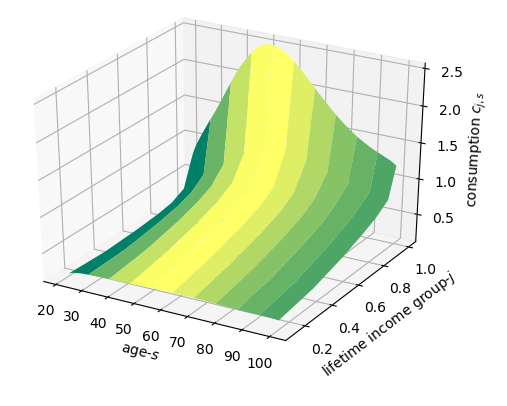
\includegraphics[width=\textwidth]{images/HHcons_SS.png}
      \caption{Consumption $\bar{c}_{j,s}$}
      \label{FigSSeqlbHHcons}
    \end{subfigure}
    \begin{subfigure}[b]{0.48\textwidth}
      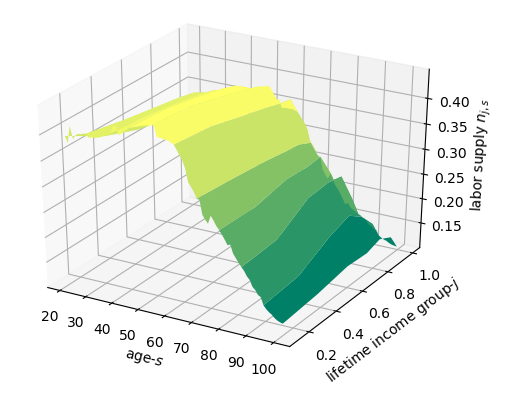
\includegraphics[width=\textwidth]{images/HHlab_SS.png}
      \caption{Labor supply $\bar{n}_{j,s}$}
      \label{FigSSeqlbHHlab}
    \end{subfigure}
    \begin{subfigure}[b]{0.48\textwidth}
      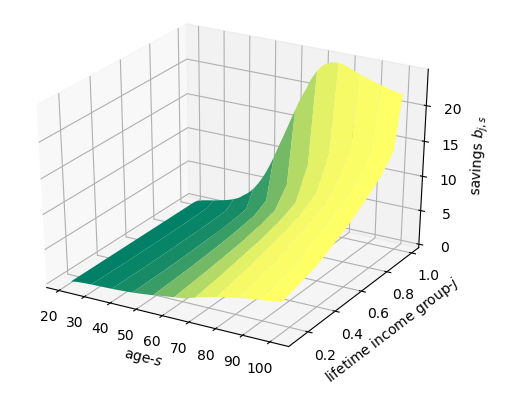
\includegraphics[width=\textwidth]{images/HHsav_SS.png}
      \caption{Savings $\bar{b}_{j,s+1}$}
      \label{FigSSeqlbHHsav}
    \end{subfigure}
  \end{figure}

  Table \ref{TabSSeqlbAggrVars} lists the steady-state prices and aggregate variable values along with some of the maximum error values from the characterizing equations.

  \begin{table}[htbp] \centering \captionsetup{width=4.1in}
  \caption{\label{TabSSeqlbAggrVars}\textbf{Steady-state prices, aggregate variables, and maximum errors}}
    \begin{threeparttable}
    \begin{tabular}{>{\small}l >{\small}r |>{\small}l >{\small}r}
      \hline\hline
      \multicolumn{1}{c}{\small{Variable}} & \multicolumn{1}{c}{\small{Value}} & \multicolumn{1}{c}{\small{Variable}} & \multicolumn{1}{c}{Value} \\
      \hline
      $\bar{r}$ & 0.058 & $\bar{w}$ & 1.148 \\
      \hline
      $\bar{Y}$ & 0.630 & $\bar{C}$ & 0.462 \\
      $\bar{I}$ & 0.144 & $\bar{K}$ & 1.810 \\
      $\bar{L}$ & 0.357 & $\bar{B}$ & 2.440 \\
      $\overline{BQ}$ & 0.106 & $factor$  & 141,580 \\
      \hline
      $\overline{Rev}$ & 0.096 & $\overline{TR}$ & 0.057 \\
      $\bar{G}$ & 0.023 & $\bar{D}$ & 0.630 \\
      \hline
      Max. abs.         & 4.57e-13 & Max. abs.  & 8.52e-13 \\[-2mm]
      \:\: labor supply &   & \:\: savings &     \\[-2mm]
      \:\: Euler error  &   & \:\: Euler error & \\
      Resource        & -4.39e-15 & Serial & 1 hr. 25.9 sec.\tnote{*} \\[-2mm]
      \:\: constraint & & \:\: computation & \\[-2mm]
      \:\: error      & & \:\: time &  \\
      \hline\hline
    \end{tabular}
    \begin{tablenotes}
      \scriptsize{\item[*]The steady-state computation time does not include any of the exogenous parameter computation processes, the longest of which is the estimation of the baseline tax functions which computation takes 1 hour and 15 minutes.}
    \end{tablenotes}
    \end{threeparttable}
  \end{table}

  \chapter{Stationary Non Steady-state Equilibrium}\label{Chap_NSSeqlb}
    %!TEX root = ../OGUSAdoc.tex

In this chapter, we define the stationary nonsteady-state equilibrium of the \ogindia model. Chapters \ref{Chap_Demog} through \ref{Chap_MarkClr} derive the equations that characterize the equilibrium of the model. We also need the steady-state solution from Chapter \ref{Chap_SSeqlb} to solve for the nonsteady-state equilibrium transition path. As with the steady-state equilibrium, we must use the stationarized version of the characterizing equations from Chapter \ref{Chap_Stnrz}.


\section{Stationary Nonsteady-State Equilibrium Definition}\label{SecEqlbNSSdef}

  We define a stationary nonsteady-state equilibrium as the following.

  \vspace{5mm}
  \hrule
  \vspace{-1mm}
  \begin{definition}[\textbf{Stationary Nonsteady-state functional equilibrium}]\label{DefNSSEql}
    A non autarkic nonsteady-state functional equilibrium in the \ogindia model is defined as stationary allocation functions of the state $\bigl\{n_{j,s,t} = \phi_s\bigl(\bm{\hat{\Gamma}}_t\bigr)\bigr\}_{s=E+1}^{E+S}$ and $\bigl\{\hat{b}_{j,s+1,t+1}=\psi_{s}\bigl(\bm{\hat{\Gamma}}_t\bigr)\bigr\}_{s=E+1}^{E+S}$ for all $j$ and $t$ and stationary price functions $\hat{w}(\bm{\hat{\Gamma}}_t)$ and $r(\bm{\hat{\Gamma}}_t)$ for all $t$ such that:
    \begin{enumerate}
      \item households have symmetric beliefs $\Omega(\cdot)$ about the evolution of the distribution of savings as characterized in \eqref{EqBeliefs}, and those beliefs about the future distribution of savings equal the realized outcome (rational expectations),
      \begin{equation*}
        \bm{\hat{\Gamma}}_{t+u} = \bm{\hat{\Gamma}}^e_{t+u} = \Omega^u\left(\bm{\hat{\Gamma}}_t\right) \quad\forall t,\quad u\geq 1
      \end{equation*}
      \item households optimize according to \eqref{EqStnrzHHeul_n}, \eqref{EqStnrzHHeul_b}, and \eqref{EqStnrzHHeul_b},
      \item firms optimize according to \eqref{EqStnrzFOC_L} and \eqref{EqFirmFOC_K},
      \item Government activity behaves according to \eqref{EqStnrzGovBC} and \eqref{EqStnrzClosureRule}, and
      \item markets clear according to \eqref{EqStnrzMarkClrLab}, \eqref{EqStnrzMarkClrCap}, and \eqref{EqStnrzMarkClrBQ}.
    \end{enumerate}
  \end{definition}
  \vspace{-2mm}
  \hrule
  \vspace{5mm}


\section{Stationary Nonsteady-state Solution Method}\label{SecEqlbNSSsoln}

  \renewcommand\theenumi{\arabic{enumi}}
  \renewcommand\theenumii{\alph{enumii}}
  \renewcommand\theenumiii{\roman{enumiii}}

  This section describes the solution method for the stationary nonsteady-state equilibrium described in Definition \ref{DefNSSEql}. We use the time path iteration (TPI) method. This method was originally outlined in a series of papers between 1981 and 1985\footnote{See \citet{AuerbachEtAl:1981,AuerbachEtAl:1983}, \citet{AuerbachKotlikoff:1983a,AuerbachKotlikoff:1983b,AuerbachKotlikoff:1983c}, and \citet{AuerbachKotlikoff:1985}.} and in the seminal book \citet[ch. 4]{AuerbachKotlikoff:1987} for the perfect foresight case and in \citet[Appendix II]{NishiyamaSmetters:2007} and \citet[Sec. 3.1]{EvansPhillips:2014} for the stochastic case. The intuition for the TPI solution method is that the economy is infinitely lived, even though the agents that make up the economy are not. Rather than recursively solving for equilibrium policy functions by iterating on individual value functions, one must recursively solve for the policy functions by iterating on the entire transition path of the endogenous objects in the economy (see \citet[ch. 17]{StokeyLucas1989}).

  The key assumption is that the economy will reach the steady-state equilibrium $\bm{\bar{\Gamma}}$ described in Definition \ref{DefSSEql} in a finite number of periods $T<\infty$ regardless of the initial state $\bm{\hat{\Gamma}}_1$. The first step in solving for the nonsteady-state equilibrium transition path is to solve for the steady-state using the method described in Section \ref{SecEqlbSSsoln}. After solving for the steady-state, one must then find a fixed point over the entire path of endogenous objects.  We do this by first making an initial guess at these objects in a the general equilibrium ``outer loop'' step, analogous to the outer loop described in the steady-state solution method. The time path iteration method then uses functional iteration to converge on a fixed point for the path of these objects.  The paths of aggregate variables that must be guessed in this outer loop are $\{\bm{r}^i,\bm{\hat{w}}^i,\bm{\hat{BQ}}^i, \bm{\hat{TR}}^i\}$, where $\bm{r}^i = \left\{r_1^i,r_2^i,...r_T^i\right\}$, $\bm{\hat{BQ}}^i = \left\{\hat{BQ}_1^i,\hat{BQ}_2^i,...\hat{BQ}_T^i\right\}$, and $\bm{\hat{TR}}^i = \left\{\hat{TR}_1^i,\hat{TR}_2^i,...\hat{TR}_T^i\right\}$. The only requirement on these transition paths is that the initial total bequests $\hat{BQ}_1^i$ conform to the initial state of the economy $\bm{\hat{\Gamma}}_1$, and that the economy has reached the steady-state by period $t=T$ $\{r_T^i, \hat{BQ}_T^i, \hat{TR}_T^i\} = \{\bar{r}, \bar{w}, \overline{BQ}, \overline{TR}\}$.

  The ``inner loop'' of the nonsteady-state transition path solution method is to solve for the full set of lifetime savings decisions $\bar{b}_{j,s+1,t+1}$ and labor supply decisions $\bar{n}_{j,s,t}$ for every household alive between periods $t=1$ and $t=T$.  To solve for the $2JS$ equations and unknowns for each household's lifetime decisions we use a multivariate root finder.

  We outline the stationary non-steady state solution algorithm in the following steps.

  \begin{enumerate}
    \item Compute the steady-state solution $\{\bar{n}_{j,s},\bar{b}_{j,s}\}_{s=E+1}^{E+S}$ corresponding to Definition \ref{DefSSEql}.

    \item Given initial state of the economy $\bm{\hat{\Gamma}}_1$ and steady-state solutions $\{\bar{n}_{j,s},\bar{b}_{j,s+1}\}_{s=E+1}^{E+S}$, guess transition paths of outer loop macroeconomic variables $\{\bm{r}^i,\bm{\hat{BQ}}^i, \bm{\hat{TR}}^i\}$ such that $\hat{BQ}_1^i$ is consistent with $\bm{\hat{\Gamma}}_1$ and $\{r_t^i, \hat{BQ}_t^i, \hat{TR}_t^i\} = \{\bar{r}, \overline{BQ}, \overline{TR}\}$ for all $t\geq T$.

    \item Given initial condition $\bm{\hat{\Gamma}}_1$, guesses for the aggregate time paths $\{\bm{r}^i,\bm{\hat{BQ}}^i, \bm{\hat{TR}}^i\}$, we solve for the inner loop lifetime decisions of every household that will be alive across the time path $\{n_{j,s,t},\hat{b}_{j,s+1,t+1}\}_{s=E+1}^{E+S}$ for all $j$ and $1\leq t\leq T$.
    \begin{enumerate}
      \item Given time path guesses $\{\bm{r}^i,\bm{\hat{BQ}}^i, \bm{\hat{TR}}^i\}$, we can compute the path of wages, $\bm{w}^i$ and then solve for each household's lifetime decisions $\{n_{j,s,t},\hat{b}_{j,s+1,t+1}\}_{s=E+1}^{E+S}$ for all $j$, $E+1\leq s \leq E+S$, and $1\leq t\leq T_2+S-1$.
      \begin{enumerate}
        \item The household problem can be solved with a multivariate root finder solving the $2S$ equations and unknowns at once for all $j$ and $1\leq t\leq T+S-1$. The root finder uses $2S$ household Euler equations \eqref{EqStnrzHHeul_n}, \eqref{EqStnrzHHeul_b}, and \eqref{EqStnrzHHeul_bS} to solve for each household's $2S$ lifetime decisions.
        \item After solving the first iteration of time path iteration, subsequent initial values for the $J$, $2S$ root finding problems are based on the solution in the prior iteration. This speeds up computation further and makes the initial guess for the highly nonlinear system of equations start closer to the solution value.
      \end{enumerate}
    \end{enumerate}
    \item Given partial equilibrium household nonsteady-state solutions $\{n_{j,s,t},\hat{b}_{j,s+1,t+1}\}_{s=E+1}^{E+S}$ for all $j$ and $1\leq t\leq T$ based on macroeconomic variable time path guesses $\{\bm{r}^i,\bm{\hat{BQ}}^i, \bm{\hat{TR}}^i\}$, compute new values for these aggregates implied by the households' solutions, $\{\bm{r}^{i'},\bm{\hat{BQ}}^{i'}, \bm{\hat{TR}}^{i'}\}$.
    \begin{enumerate}
          \item We solve for the updated interest rate as follows:
    		\begin{enumerate}
    			\item Use the guess at the path of total transfers, $\hat{TR}_{t}^{i}$ and the transfer spending rule given in Equation \eqref{EqUnbalGBCtfer} to find the implied path of GDP: $\hat{Y}_{t}^{i} = \frac{\hat{TR}_{t}^{i}}{\alpha_{tr}}$.
    			\item Using the path of GDP and the household savings and labor supply decisions, $\{n_{j,s,t},\hat{b}_{j,s+1,t+1}\}_{s=E+1}^{E+S}$, compute the path of stationarizaed total tax revenue, $\hat{Revenue}_{t}^{i}$.
    			\item Using the long-run debt-to-GDP ratio, the path of GDP, the path of total tax revenue, and Equation \eqref{EqUnbalGBCclosure_Gt}, find the path of stationarized government debt, $\hat{D}_{t}^{i}$.
    			\item Use the capital market clearing condition from Equation \eqref{EqStnrzMarkClrCap} and $D_{t}^{i}$ to find aggregate capital in each period,

    			\begin{equation*}
    				\hat{K}_{t}^{i}=\frac{1}{1 + g_{n,t}}\sum_{s=E+2}^{E+S+1}\sum_{j=1}^{J}\Bigl(\omega_{s-1,t-1}\lambda_j \hat{b}_{j,s,t} + i_s\omega_{s,t}\lambda_j \hat{b}_{j,s,t}\Bigr) - D_{t}^{i}
    			\end{equation*}

    		\item Use the labor market clearing condition from Equation \eqref{EqStnrzMarkClrLab} to find the path of aggregate labor supply:

    			\begin{equation*}
    				\hat{L}_{t}^{i}=\sum_{s=E+1}^{E+S}\sum_{j=1}^{J} \omega_{s,t}\lambda_j e_{j,s}n_{j,s,t}
    			\end{equation*}

    		\item Use the firm's production function from Equation \eqref{EqStnrzCESprodfun} to compute an updated value of $\hat{Y}_{t}$ given the values for the factors of production:

    		\begin{equation*}
    			\hat{Y}_{t}^{i'} = Z_{t}\biggl[(\gamma)^\frac{1}{\ve}(\hat{K}_{t}^{i})^\frac{\ve-1}{\ve} + (1-\gamma)^\frac{1}{\ve}(\hat{L}_{t}^{i})^\frac{\ve-1}{\ve}\biggr]^\frac{\ve}{\ve-1}
    		\end{equation*}

    		\item Use the firm's first order condition for its choice of capital to find the updated path of interest rates,

    		\begin{equation*}
    			r_{t}^{i'} = (1 - \tau_{t}^{corp})(Z_{t})^\frac{\ve-1}{\ve}\left[\gamma\frac{\hat{Y}_{t}^{i'}}{\hat{K}_{t}^{i}}\right]^\frac{1}{\ve} - \delta + \tau_{t}^{corp}\delta_{t}^\tau
    		\end{equation*}

    	\end{enumerate}

    	\item The stationarized law of motion for total bequests \eqref{EqStnrzMarkClrBQ} provides the expression in which household savings decisions $\{b_{j,s+1,t+1}\}_{s=E+1}^{E+S}$ imply a value for aggregate bequests, $BQ_{t}^{\,i'}$. When computing aggregate bequests, we use the updated path of interest rates found above.
    		\begin{equation*}
    			\hat{BQ}_{t}^{\,i'} = \left(\frac{1+r_{t}^{i'}}{1 + g_{n,t}}\right)\left(\sum_{s=E+2}^{E+S+1}\sum_{j=1}^J\rho_{s-1}\lambda_j\omega_{s-1,t-1}\hat{b}_{j,s,t}\right)
    		\end{equation*}

    	\item In equation \eqref{EqStnrzTfer}, we defined total household transfers as a fixed percentage of GDP ($\hat{TR}_t=\alpha_{tr}\hat{Y}_t$).  To find the updated value for transfers, we find the amount of transfers implied by the most updated value of GDP, $\hat{TR}_{t}^{i'}=\alpha_{tr}\hat{Y}_{t}^{i'}$.



	\end{enumerate}
	\item The updated values for the outer loop variables are then used to compute the percentage differences between the initial and implied values:
		\begin{enumerate}
			\item $error_r = max\left\{\frac{r_{t}^{i'} - r_{t}^i}{r_{t}^i}\right\}_{t=0}^{T}$
			\item $error_{bq} =  max\left\{\frac{\hat{BQ}_{t}^{\,i'} - \hat{BQ}_{t}^{\,i}}{\hat{BQ}_{t}^{\,i}}\right\}_{t=0}^{T}$
			\item $error_{tr} = \left\{\frac{\hat{TR}_{t}^{\,i'} - \hat{TR}_{t}^{\,i}}{\hat{TR}_{t}^{\,i}}\right\}_{t=0}^{T}$
		\end{enumerate}
	\item If the maximum absolute error among the three outer loop error terms is greater than some small positive tolerance $toler_{tpi,out}$,
		\begin{equation*}
			\max\big|\left(error_r,error_{bq},error_{tr},error_f\right)\bigr| > toler_{tpi,out}
		\end{equation*}
	then update the guesses for the outer loop variables as a convex combination governed by $\xi_{tpi}\in(0,1]$ of the respective initial guesses and the new implied values and repeat steps (3) through (5).
	\begin{equation*}
		\begin{split}
			\left[\bm{r}^{i+1},\bm{\hat{BQ}}^{\,i+1},\bm{\hat{TR}}^{\,i+1}\right] &= \xi_{tpi}\left[\bm{r}^{i'},\bm{\hat{BQ}}^{\,i'},\bm{\hat{TR}}^{\,i'}\right] + \\
			&\qquad(1-\xi_{tpi})\left[\bm{r}^{i},\bm{\hat{BQ}}^{\,i},\bm{\hat{TR}}^{\,i}\right]
		\end{split}
	\end{equation*}
	\item If the maximum absolute error among the five outer loop error terms is less-than-or-equal-to some small positive tolerance $toler_{tpi,out}$ in each period along the transition path,
		\begin{equation*}
			\max\big|\left(error_r,error_{bq},error_{tr},error_f\right)\bigr| \leq toler_{tpi,out}
		\end{equation*}
	then the non-steady-state equilibrium has been found.
		\begin{enumerate}
			\item Make sure that the resource constraint (goods market clearing) \eqref{EqStnrzMarkClrGoods} is satisfied in each period along the time path. It is redundant, but this is a good check as to whether everything worked correctly.
			\item Make sure that the government budget constraint \eqref{EqStnrzGovBC} binds.
			\item Make sure that all the $(T+S)\times2JS$ household Euler equations are solved to a satisfactory tolerance.
		\end{enumerate}
  \end{enumerate}

  \renewcommand\theenumi{\roman{enumi}}


\section{Baseline Nonsteady-state Results}\label{SecNSSeqlbResults}

  asdf


\part{Calibration and International Options}\label{PartSolMthCal}
  \chapter{Calibration}\label{Chap_Calibr}
    % \input{Chapters/Chap_Calibr}
  \chapter{Open Economy Specifications}\label{Chap_SmOpEcn}
    %!TEX root = ../OGUSAdoc.tex

\section{Small Open Economy}
In the small open economy version of \ogindia, the county faces an exogenous world interest rate, $r^{*}_{t}$ that determines the amount of savings and investment.  If the supply of savings from households does not meet the demand for private capital and private borrowing, foreign capital will flow in to make excess demand zero at the world interest rate.  Let the total capital stock be given by the quantity of domestically supplied capital and foreign supplied capital, i.e., $K_{t}= K^{d}_{t}+K^{f}_{t}$.  Then foreign capital is given by:

\begin{equation}
  K^{f}_{t} = K^{demand}_{t} - B_{t} - D_{t},
\end{equation}

where $B_{t}$ is aggregate household savings and $D_{t}$ is government borrowing.  Capital demand is determined from the firm's first order condition for its choice of capital.

\section{Partially Open Economy}

In the partially open economy version of \ogindia, the openness of the economy is modeled through two parameters that capture the extent of foreign lending to the domestic government and the amount of foreign lending of private capital to firms.


The parameter $\zeta_{D}$ gives the share of new debt issues that are purchased by foreigners.  The law of motion for foreign-held debt is therefore given by:

\begin{equation}
  D^{f}_{t+1} = D^{f}_{t} + \zeta_{D}(D_{t+1} - D_{t})
\end{equation}

Domestic debt holdings as then the remaining debt holdings needed to meet government demand for debt:

\begin{equation}
  D^{d}_{t} = D_{t} - D^{f}_{t}
\end{equation}


The parameters $\zeta_{K}$ helps to determine the share of domestic capital held by foreigners.  In particular, $\zeta_{D}$ is the share of foreign capital held by foreigners in the small open economy specification:

\begin{equation}
  K^{f}_{t} = \zeta_{K}K^{open}_{t}
\end{equation}

$K^{open}_{t}$ is the amount of capital that would need to flow into the country to meet firm demand for capital at the exogenous world interest rate from the small open economy specification, net of what domestic households can supply:

\begin{equation}
  K^{open}_{t} = K^{demand, open}_{t} - (B_{t} - D^{d}_{t})
\end{equation}

where, $K^{demand, open}_{t}$ is total capital demand by domestic firms at $r^
{*}_{t}$, $B_{t}$ are total asset holdings of domestic households, and $D^{d}_{t}$ are holdings of government debt by domestic households.  Total asset holdings from households result from solving the household problem at the endogenous home country interest rate.  Note that there is a disconnect between the interest rates that determine firm capital demand and domestic household savings and the interest rate used to determine $K^{demand, open}_{t}$.  This assumption is useful in that it nests the small open economy case into the partial open economy model.  However, it does leave out the realistic responses of foreign capital supply to differentials in the home country interest rate and the world interest rate.

Given the two equations above, we can find the total supply of capital as:

\begin{equation}
  \begin{split}
  K^{supply}_{t} & = K^{d}_{t} + K^{f}_{t} \\
   & = B_{t} - D^{d}_{t} + \zeta_{K}K^{open}_{t} \\
  \end{split}
\end{equation}


\subsection{Stationarization}

\subsubsection{Foreign debt purchases}

The amount of government debt is growing by the rate of productivity growth and the rate of population growth.  Thus, stationarized government debt is given by:

\begin{equation}
  \hat{D}_{t} = \frac{D_{t}}{e^{g_{y}t}N_{t}}
\end{equation}

The stationarized form of the foreign and domestic capital holdings thus become:

\begin{equation}
  \begin{split}
    \hat{D}^{f}_{t+1} & = \frac{D^{f}_{t+1}}{e^{g_{y}t+1}N_{t+1}} = \frac{D^{f}_{t}}{e^{g_{y}t+1}N_{t+1}} + \zeta_{D}(\frac{D_{t+1}}{e^{g_{y}t+1}N_{t+1}} - \frac{D_{t}}{e^{g_{y}t+1}N_{t+1}}) \\
    & = \frac{\hat{D}^{f}_{t}N_{t}}{e^{g_{y}}N_{t+1}} + \zeta_{D}(\hat{D}_{t+1} - \frac{\hat{D}_{t}N_{t}}{e^{g_{y}}N_{t+1}}) = \frac{\hat{D}^{f}_{t}}{e^{g_{y}}g_{n,t+1}} + \zeta_{D}(\hat{D}_{t+1} - \frac{\hat{D}_{t}}{e^{g_{y}}g_{n,t+1}})
  \end{split}
\end{equation}

and

\begin{equation}
  \hat{D}^{d}_{t} = \frac{D^{d}_{t}}{e^{g_{y}t}N_{t}} = \frac{D_{t}}{e^{g_{y}t}N_{t}} - \frac{D^{f}_{t}}{e^{g_{y}t}N_{t}} = \hat{D}_{t} - \hat{D}^{f}_{t}
\end{equation}


Note that in the steady-state, we still have $\hat{D}^{f} = \zeta_{D}\hat{D}$


\subsubsection{Foreign capital purchase}

In the equation for foreign capital purchases, all quantities are growing at the rate of technological change and population growth.  Thus, to stationarize this equation, we find:

\begin{equation}
  \hat{K}^{f}_{t} = \frac{K^{f}_{t}}{e^{g_{y}t}N_{t}}= \zeta_{K}\frac{K^{open}_{t}}{e^{g_{y}t}N_{t}} = \zeta_{K}\hat{K}^{open}_{t}
\end{equation}

and

\begin{equation}
  \hat{K}^{open}_{t} = \frac{K^{open}_{t}}{e^{g_{y}t}N_{t}}= \frac{K^{demand, open}_{t}}{e^{g_{y}t}N_{t}} - \left(\frac{B_{t}}{e^{g_{y}t}N_{t}} - \frac{D^{d}_{t}}{e^{g_{y}t}N_{t}}\right) = \hat{K}^{demand, open}_{t} - (\hat{B}_{t}-\hat{D}_{t})
\end{equation}

and

\begin{equation}
  \begin{split}
  \hat{K}^{supply}_{t} &= \frac{K^{supply}_{t}}{e^{g_{y}t}N_{t}} = \frac{K^{d}_{t}}{e^{g_{y}t}N_{t}} + \frac{K^{f}_{t}}{e^{g_{y}t}N_{t}} = \hat{K}^{d}_{t} + \hat{K}^{f}_{t} \\
   & = \frac{B_{t}}{e^{g_{y}t}N_{t}} - \frac{D^{d}_{t}}{e^{g_{y}t}N_{t}} + \zeta_{K}\frac{K^{open}_{t}}{e^{g_{y}t}N_{t}} = \hat{B}_{t} - \hat{D}^{d}_{t} + \zeta_{K}\hat{K}^{open}_{t} \\
  \end{split}
\end{equation}

\subsubsection{Resource Constraint}

As a result of the foreign ownership of capital, the resource constraint is modified.  In a closed economy, the resource constraint is given by:

\begin{equation}
  Y_{t} = C_{t} + I_{t} + G_{t}
\end{equation}

In the partially open economy, some of the output is paid to the foreign owners of capital.  This amount is given by $r_{t}K^{f}_{t}$.  In addition, foreign lending to the home country's government relaxes the resource constraint.  In the case , the resource constraint is given by:

\begin{equation}
  Y_{t} = C_{t} + (K^{d}_{t+1} - K^{d}_{t}) + \delta K_{t} +  G_{t} + r_{t}K^{f}_{t} - (D^{f}_{t+1}-D^{f}_{t}) + rD^{f}_{t}
\end{equation}

The stationarized version of this becomes:

\begin{equation}
  \hat{Y}_{t} = \hat{C}_{t} + (\hat{K}^{d}_{t+1}e^{g_{y}}(1+g_{n,t+1}) - \hat{K}^{d}_{t}) + \delta \hat{K}_{t} +  \hat{G}_{t} + r_{t}\hat{K}^{f}_{t} - (\hat{D}^{f}_{t+1}e^{g_{y}}(1+g_{n,t+1})- \hat{D}^{f}_{t}) + r_{t}\hat{D}^{f}_{t}
\end{equation}

Note that with a wedge between the interest rate on government debt and private capital as outlined in Chapter \ref{SecRateWedge} we need to be careful about the interest rates paid and the amount of capital and debt held.  In the case of the partially open economy with an interest rate wedge, we assume that domestic and foreign investors earn a rate of return on their portfolio of:

\begin{equation}
  r_{hh,t} = \frac{r_{t}K_{t} + r_{gov,t}D_{t}}{K_{t} + D_{t}}
\end{equation}

In the partially open economy, the ratio of private capital to debt held by domestic households might differ from the ratio held by foreign households, but we assume they still earn the same rate of return on their portfolio.\footnote{One reason for this assumption is that it simplifies our solution since we do not need to know the domestic versus foreign holdings of capital before solving the households' problems.}  With this assumption, we modify the resource constraint to be a function of this portfolio interest rate:

\begin{equation}
  \hat{Y}_{t} = \hat{C}_{t} + (\hat{K}^{d}_{t+1}e^{g_{y}}(1+g_{n,t+1}) - \hat{K}^{d}_{t}) + \delta \hat{K}_{t} +  \hat{G}_{t} + r_{hh, t}\hat{K}^{f}_{t} - (\hat{D}^{f}_{t+1}e^{g_{y}}(1+g_{n,t+1})- \hat{D}^{f}_{t}) + r_{hh,t}\hat{D}^{f}_{t}
\end{equation}



\appendix
\appendixpage
\addappheadtotoc

\chapter{Derivations}\label{Chap_Deriv}
  %!TEX root = ../OGUSAdoc.tex

This appendix contains derivations from the theory in the body of this book.


\section{Properties of the CES Production Function}\label{SecAppDerivCES}

  The constant elasticity of substitution (CES) production function of capital and labor was introduced by \citet{Solow:1956} and further extended to a consumption aggregator by \citet{Armington:1969}. The CES production function of aggregate capital $K_t$ and aggregate labor $L_t$ we use in Chapter \ref{Chap_Firms} is the following,
  \begin{equation}\tag{\ref{EqFirmsCESprodfun}}
    Y_t = F(K_t, L_t) \equiv Z_t\biggl[(\gamma)^\frac{1}{\ve}(K_t)^\frac{\ve-1}{\ve} + (1-\gamma)^\frac{1}{\ve}(e^{g_y t}L_t)^\frac{\ve-1}{\ve}\biggr]^\frac{\ve}{\ve-1} \quad\forall t
  \end{equation}
  where $Y_t$ is aggregate output (GDP), $Z_t$ is total factor productivity, $\gamma$ is a share parameter that represents the capital share of income in the Cobb-Douglas case ($\ve=1$), and $\ve$ is the elasticity of substitution between capital and labor. The stationary version of this production function is given in Chapter \ref{Chap_Stnrz}. We drop the $t$ subscripts, the ``$\:\hat{\,}\:$''stationary notation, and use the stationarized version of the production function \eqref{EqStnrzCESprodfun} for simplicity.
  \begin{equation}\tag{\ref{EqStnrzCESprodfun}}
    Y =  Z\biggl[(\gamma)^\frac{1}{\ve}(K)^\frac{\ve-1}{\ve} + (1-\gamma)^\frac{1}{\ve}(L)^\frac{\ve-1}{\ve}\biggr]^\frac{\ve}{\ve-1}
  \end{equation}
  The Cobb-Douglas production function is a nested case of the general CES production function with unit elasticity $\ve=1$.
  \begin{equation}\label{EqAppDerivCES_CobbDoug}
    Y = Z(K)^\gamma(L)^{1-\gamma}
  \end{equation}



  \subsection{Wages as a function of interest rates}\label{SecAppDerivCESwr}

    An important property of the CES production function for the solution method of \ogindia is that the interest rate $r_t$ and wage $w_t$ are functions of the capital labor ratio. This property implies that the wage every period $w_t$ is just a function of the interest rate $r_t$, and vice versa. The first step is to show that the output-capital ratio ($Y/K$) and the output-labor ($Y/L$) ratio are both functions of the capital-labor ratio ($K/L$).
    \begin{equation}\label{EqAppDerivCES_YL}
      \begin{split}
      Y &= Z\biggl[(\gamma)^\frac{1}{\ve}(K)^\frac{\ve-1}{\ve} + (1-\gamma)^\frac{1}{\ve}(L)^\frac{\ve-1}{\ve}\biggr]^\frac{\ve}{\ve-1} \\
      &= Z\left[(\gamma)^\frac{1}{\ve}(K)^\frac{\ve-1}{\ve}\left(\frac{L^\frac{\ve-1}{\ve}}{L^\frac{\ve-1}{\ve}}\right) + (1-\gamma)^\frac{1}{\ve}(L)^\frac{\ve-1}{\ve}\right]^\frac{\ve}{\ve-1} \\
      &= ZL\left[(\gamma)^\frac{1}{\ve}\left(\frac{K}{L}\right)^\frac{\ve-1}{\ve} + (1-\gamma)^\frac{1}{\ve}\right]^\frac{\ve}{\ve-1} \\
      \Rightarrow\quad \frac{Y}{L} &= Z\left[(\gamma)^\frac{1}{\ve}\left(\frac{K}{L}\right)^\frac{\ve-1}{\ve} + (1-\gamma)^\frac{1}{\ve}\right]^\frac{\ve}{\ve-1}
      \end{split}
    \end{equation}

    \begin{equation}\label{EqAppDerivCES_YK}
      \begin{split}
      Y &= Z\biggl[(\gamma)^\frac{1}{\ve}(K)^\frac{\ve-1}{\ve} + (1-\gamma)^\frac{1}{\ve}(L)^\frac{\ve-1}{\ve}\biggr]^\frac{\ve}{\ve-1} \\
      &= Z\left[(\gamma)^\frac{1}{\ve}(K)^\frac{\ve-1}{\ve} + (1-\gamma)^\frac{1}{\ve}(L)^\frac{\ve-1}{\ve}\left(\frac{K^\frac{\ve-1}{\ve}}{K^\frac{\ve-1}{\ve}}\right)\right]^\frac{\ve}{\ve-1} \\
      &= ZK\left[(\gamma)^\frac{1}{\ve} + (1-\gamma)^\frac{1}{\ve}\left(\frac{L}{K}\right)^\frac{\ve-1}{\ve}\right]^\frac{\ve}{\ve-1} \\
      \Rightarrow\quad \frac{Y}{K} &= Z\left[(\gamma)^\frac{1}{\ve} + (1-\gamma)^\frac{1}{\ve}\left(\frac{L}{K}\right)^\frac{\ve-1}{\ve}\right]^\frac{\ve}{\ve-1}
      \end{split}
    \end{equation}

    Solving for the firm's first order conditions for capital and labor demand from profit maximization \eqref{EqStnrzProfit} gives the following equations in their respective stationarized forms from Chapter \ref{Chap_Stnrz}.
    \begin{align}
      w &= (Z)^\frac{\ve-1}{\ve}\left[(1-\gamma)\left(\frac{Y}{L}\right)\right]^\frac{1}{\ve} \tag{\ref{EqStnrzFOC_L}} \\
      r &= (1 - \tau^{corp})(Z)^\frac{\ve-1}{\ve}\left[\gamma\left(\frac{Y}{K}\right)\right]^\frac{1}{\ve} - \delta + \tau^{corp}\delta^\tau \tag{\ref{EqFirmFOC_K}}
    \end{align}
    As can be seen from \eqref{EqStnrzFOC_L} and \eqref{EqFirmFOC_K}, the wage $w$ and interest rate $r$ are functions of $Y/L$ and $Y/K$, respectively. Equations \eqref{EqAppDerivCES_YL} and \eqref{EqAppDerivCES_YK} show that both $Y/L$ and $Y/K$ are functions of the capital-labor ratio $K/L$. Substituting \eqref{EqAppDerivCES_YL} and \eqref{EqAppDerivCES_YK} into \eqref{EqStnrzFOC_L} and \eqref{EqFirmFOC_K}, respectively, gives expressions of the wage $w$ and interest rate $r$ in terms of the capital-labor ratio $K/L$.
    \begin{align}
      w &= (1-\gamma)^\frac{1}{\ve}Z\left[(\gamma)^\frac{1}{\ve}\left(\frac{K}{L}\right)^\frac{\ve-1}{\ve} + (1-\gamma)^\frac{1}{\ve}\right]^\frac{1}{\ve-1} \label{EqAppDerivCES_FOCL} \\
      r &= (1 - \tau^{corp})(\gamma)^\frac{1}{\ve}Z\left[(\gamma)^\frac{1}{\ve} + (1-\gamma)^\frac{1}{\ve}\left(\frac{L}{K}\right)^\frac{\ve-1}{\ve}\right]^\frac{1}{\ve-1} - \delta + \tau^{corp}\delta^\tau \label{EqAppDerivCES_FOCK}
    \end{align}
    In the Cobb-Douglas unit elasticity case ($\ve=1$) of the CES production function, the first order conditions are more easily expressed in terms of the capital-labor ratio.
    \begin{align}
      \text{if}\:\:\,\ve=1:\quad w &= (1-\gamma)Z\left(\frac{K}{L}\right)^\gamma \label{EqAppDerivCES_CDFOCL} \\
      \text{if}\:\:\:\ve=1:\quad r &= (1 - \tau^{corp})\gamma Z\left(\frac{L}{K}\right)^{1-\gamma} - \delta + \tau^{corp}\delta^\tau \label{EqAppDerivCES_CDFOCK}
    \end{align}

    With $w$ and $r$ expressed in terms of the capital-labor ratio $K/L$ in \eqref{EqAppDerivCES_FOCL} and \eqref{EqAppDerivCES_FOCK}, we can write the expressions for the capital-labor ratio as a function of the interest rate and, therefore, the wage as a function of the interest rate. We first solve equation \eqref{EqAppDerivCES_FOCK} for the capital-labor ratio to get the expression for $K/L$ as a function of the interest rate $r$.
    \begin{equation}\label{EqAppDerivCES_KLr}
      \frac{K}{L} = \left(\frac{(1-\gamma)^\frac{1}{\ve}}{\left[\frac{r + \delta - \tau^{corp}\delta^\tau}{(1 - \tau^{corp})\gamma^\frac{1}{\ve}Z}\right]^{\ve-1} - \gamma^\frac{1}{\ve}}\right)^\frac{\ve}{\ve-1}
    \end{equation}
    In the Cobb-Douglas unit elasticity case ($\ve=1$), we solve equation \eqref{EqAppDerivCES_CDFOCK} for the capital-labor ration to get the expression for $K/L$ as a function of the interest rate $r$.
    \begin{equation}\label{EqAppDerivCES_CDKLr}
      \text{if}\:\:\:\ve=1:\quad \frac{K}{L} = \left[\frac{(1 - \tau^{corp})\gamma Z}{r + \delta - \tau^{corp}\delta^\tau}\right]^\frac{1}{1-\gamma}
    \end{equation}

    Substituting \eqref{EqAppDerivCES_KLr} into \eqref{EqAppDerivCES_FOCL} gives the expression for the wage $w$ as a function of the interest rate $r$ in the general CES case.
    \begin{equation}\label{EqAppDerivCES_wr}
      w = (1-\gamma)^\frac{1}{\ve}Z\left[(\gamma)^\frac{1}{\ve}\left(\frac{(1-\gamma)^\frac{1}{\ve}}{\left[\frac{r + \delta - \tau^{corp}\delta^\tau}{(1 - \tau^{corp})\gamma^\frac{1}{\ve}Z}\right]^{\ve-1} - \gamma^\frac{1}{\ve}}\right) + (1-\gamma)^\frac{1}{\ve}\right]^\frac{1}{\ve-1}
    \end{equation}
    In the Cobb-Douglas unit elasticity case ($\ve=1$), we substitute \eqref{EqAppDerivCES_CDKLr} into \eqref{EqAppDerivCES_CDFOCL} gives the expression for the wage $w$ as a function of the interest rate $r$.
    \begin{equation}\label{EqAppDerivCES_CDwr}
      \text{if}\:\:\:\ve=1:\quad w = (1-\gamma)Z\left[\frac{(1 - \tau^{corp})\gamma Z}{r + \delta - \tau^{corp}\delta^\tau}\right]^\frac{\gamma}{1-\gamma}
    \end{equation}

% \chapter{Using Python}\label{Chap_Python}
%   %!TEX root = ../OGtextbook.tex
% TODO: Place this chapter as an appendix chapter before Git chapter

Python is a powerful and elegant open-source programming language that has become widely used in scientific computing and the new field of open data science. Since its introduction in 1991, Python's internal features, libraries, and user network have expanded in ways that have made it a go-to language for prototyping processes. Its ease of integrating with compiled languages such as C and Fortran make it ideal as the master scripting language in hierarchical programs and modules. Python also has great structures and syntax that are amenable to flexible functional programming, object oriented programming, and parallel processing.

It is true that Python's ``interpreted'' language status means that it is often slower than Fortran or C. But most of the Python functions and libraries that could leverage compiled language speedups--such as root finders, optimizers, matrix inversion, and matrix decomposition---are already implemented in Python as wrappers of the optimized C and Fortran code.


\section{Installing Python}\label{SecPythonInstall}

  A basic Python kernel can be installed from \href{https://www.python.org/downloads/}{https://www.python.org/downloads/}. However, this is not the recommendation of this book. Because Python has many important libraries that can be added to the distribution, this book recommends downloading the \href{https://www.continuum.io/downloads}{Anaconda distribution} of Python (https://www.continuum.io/downloads), which is curated by Continuum Analytics. In previous years, many users remained with version 2.x despite the existence of 3.x. However, Python 3.x has now been extensively tested and widely adopted by the Python community and it is advisable to download the latest version (currently 3.x). The Anaconda distribution of Python is easy to install on Mac OS X, Windows, and Linux machines.


\section{Learning Python}\label{SecPythonLearning}

  Many resources exist for learning Python. Most widely used are the online tutorials. Below are some favorite examples.

  \begin{itemize}
    \item \href{https://docs.python.org/3/tutorial/}{The official Python 3 tutorial site} (https://docs.python.org/3/tutorial/)
    \item \href{https://www.codecademy.com/learn/python}{Code Academy's Python learning module} (https://www.codecademy.com/learn/python)
    \item \href{http://lectures.quantecon.org/py/index.html}{Quant-Econ.net} tutorial of how to use Python for Economics applications (http://lectures.quantecon.org/py/index.html)
    \item Applied and Computational Mathematics Emphasis at Brigham Young University \href{http://www.acme.byu.edu/?page\_id=2067}{open source Python training labs} (http://www.acme.byu.edu/?page\_id=2067)
  \end{itemize}

  In addition, a number of excellent textbooks and reference manuals are very helpful and may be available in your local library. Or you may just want to have these in your own library. \citet{Lutz:2013} is a giant 1,500-page reference manual that has an expansive collection of materials targeted at beginners. \citet{Beazley:2009} is a more concise reference but is targeted at readers with some experience using Python. Despite its focus on a particular set of tools in the Python programming language, \citet{McKinney:2013} has a great introductory section that can serve as a good starting tutorial. Further, its focus on Python's data analysis capabilities is truly one of the important features of Python. Rounding out the list is \citet{Langtangen:2010}. This book's focus on scientists and engineers makes it a unique reference for optimization, wrapping C and Fortran and other scientific computing topics using Python.

  As with any programming language, the long-run internalized learning comes from using the language in relevant applications. This book will provide many economic applications of a broad set of computational tools using Python. These tools are applicable in many other fields. And they can be implemented in other programming languages. But Python currently occupies a strong niche of being a programming language with broad capabilities, having an active and expanding user group, having a syntax that is efficient and relatively easy to write, and being open source. From a general standpoint, it is likely that Python's use will continue expanding in economics.


\section{Principles of Writing Good Code}\label{SecPythonPrinc}

  \begin{itemize}
    \item Python has its own preferred style of writing good code. These best practices are listed in \href{https://www.python.org/dev/peps/pep-0008/}{PEP 8 -- Style Guide for Python Code} (https://www.python.org/dev/peps/pep-0008/).\footnote{PEP stands for ``Python Enhancement Proposals''.}
    \item Work with 1-dimensional arrays or numpy vectors as much as possible. For example, a vector $x$ with $n$ elements should have shape \texttt{x.shape = (n,)}. In addition, some operations on matrix $\bm{A}$ with $m$ rows and $n$ columns can be more efficiently executed by vectorizing $\bm{A}$ or transforming it into a one-dimensional array $a$ with $m\times n$ elements.
    \item Write functions for particular lines of code that get reused and represent a clear concept from the theory. This is an art of understanding efficient coding. It also means that if you change a concept or augment your code, you might only have to make the change in one place even though that concept gets used in the code in multiple places.
    \item Avoid using global variables across functions.
    \item Use Python tuples to pass arguments between functions because the data types can vary across tuple elements (e.g., you can pack integer elements with float elements).
    \item Learn how to use the \texttt{*args} and \texttt{**kwargs} constructs in passing tuples of varying lengths into functions.
    \item Store sets of functions in intuitive groups in separate python script (\texttt{file.py}) files. These scripts are called modules. Import these functions when needed by importing the module using \texttt{import file as fl}. Then you can call those functions in your current script using \texttt{fl.funcname(...)}.
    \item Place comments and meta data extensively throughout your code. Every function should have explanations of what the function does, what are the inputs, what functions are called, what objects are created inside the function, and what is the output of the function. This will feel like overkill at the beginning, but it will save you and everyone else who every uses your code lots of time over the long run. \href{https://www.python.org/dev/peps/pep-0257/}{PEP 257} (https://www.python.org/dev/peps/pep-0257/) provides a description of Python docstring and meta data conventions.
    \item Use the theory to map out what the optimal structure of your code should be. A universal principle in scientific computing is that insights, efficiency, and discovery can happen going both from theory to computation as well as from computation to theory. Use them both extensively. If you have a problem in the code, it might be highlighting an issue in the theory. If you have a problem in the theory, you might be able to discover the reason by computing different scenarios and special cases.
    \item Use parallelization where possible. Python's \texttt{multiprocessing} library makes this very easy on your own machine. For more advanced and flexible parallel processing, the \texttt{mpi4py} library imports tools for implementing MPI (message passing interface) operations.
  \end{itemize}


\section{Running Python}\label{SecPythonRun}

  asdf

  \subsection{Text editor and terminal}\label{SecPythonRunText}

    Talk about Vim, Emacs, Sublime Text 3.


  \subsection{IDE}\label{SecPythonRunIDE}

    Spyder is like MATLAB. ipython


  \subsection{Jupyter Notebook}\label{SecPythonRunJupyt}

    Jupyter is a general platform that can display ``notebooks'' in your browser that can interactively run code in a number of languages and can display other surrounding rich text elements such as text, equations, figures, and links. Jupyter notebooks are ideal for teaching programming and giving examples because they can be executed and manipulated in real time and they can be saved as a record for future use. I will use Jupyter notebooks in class to teach some of the computational techniques you will be using in your problem sets. I will save these notebooks to the class GitHub repository.

    If you have installed the Anaconda distribution of Python on your computer, you can open the Jupyter notebook server dashboard by going to your terminal and typing \texttt{jupyter notebook}. If you do not have the Anaconda distribution of Python, you can install Jupyter by following the instructions at \href{http://jupyter.readthedocs.io/en/latest/install.html}{http://jupyter.readthedocs.io/en/latest/install.html}. The \href{https://jupyter-notebook-beginner-guide.readthedocs.io/en/latest/}{Jupyter/IPython Notebook Quick Start Guide} (https://jupyter-notebook-beginner-guide.readthedocs.io/en/latest/) provides a nice introduction to installing and using the Jupyter notebook system.

    You can open a Jupyter notebook by navigating in your terminal to the directory on your local computer in which a Jupyter notebook is saved. Type the following command in your terminal to open the Jupyter server dashboard.
    \begin{lstlisting}[frame=single]
      >>> jupyter notebook
    \end{lstlisting}
    As shown in Figure \ref{FigPythonJupInit}, the Jupyter dashboard interface will show all of the files available in that directory. To open one of the Jupyter notebooks, simply double click on the desired file with the ``.ipynb'' file-type suffix.

    \begin{figure}[htbp]\centering\captionsetup{width=6.0in}
      \caption{\textbf{Screenshot of Jupyter startup dashboard}}\label{FigPythonJupInit}
      \fbox{\resizebox{6.0in}{1.8in}{\includegraphics{./images/JupyterDash.png}}}
    \end{figure}


\section{Debugging}\label{SecPythonDebug}

  \begin{itemize}
    \item Debugging is unavoidable.
    \item Develop an endurance to stick with the problem until it is solved.
    \item Coding errors go down with experience, holding ability constant.
      \begin{itemize}
        \item Coding ability usually rises over time, which means that it is not clear that debugging ever goes away.
      \end{itemize}
    \item Stackoverflow is your friend.
  \end{itemize}


\section{Python cheat sheet}\label{SecPythonCheat}

  In this section, I list a number of useful Python commands that are not as frequently used.
  \begin{itemize}
    \item How to set IPython to automatically reload modules that had previously been imported. Load the IPython \texttt{autoreload} extension by typing the following two Python magic function commands.
    \begin{lstlisting}[frame=single]
      >>> %load_ext autoreload
      >>> %autoreload 2
    \end{lstlisting}
  \end{itemize}


\section{Optimization: Root Finders and Minimizers}\label{SecPythonOpt}

  Root finders and minimizers are the two key tools for solving numerical optimization problems. We will define the general formulation of an optimization problem as a minimization problem,
  \begin{equation}\label{EqPythonOptGen}
    \min_{\bm{x}}\: f\left(\bm{x},\bm{z}|\bm{\theta}\right) \quad\text{s.t}\quad \bm{g}(\bm{x},\bm{z}|\bm{\theta})\geq\bm{0} \quad\text{and}\quad \bm{h}(\bm{x}) = \bm{0}
  \end{equation}
  where $\bm{x}=\{x_1, x_2,... x_N\}$ is a vector of $N$ endogenous variables, $\bm{z}$ is a vector of exogenous variables, $\bm{\theta}$ is a vector of model parameters, $f$ is a scalar-valued potentially nonlinear function of $(\bm{x},\bm{z})$ given parameters $\bm{\theta}$, $\bm{g}$ is a system of $K$ potentially nonlinear inequality constraints, and $\bm{h}$ is a system of $J$ potentially nonlinear equality constraints.

  An example of a minimization problem of the form \eqref{EqPythonOptGen} is the 3-period lived agent OG model with exogenous labor supply in Chapter \ref{Chap_3perSimp}. Each household's optimization problem is the following.
  \begin{equation}\label{EqPython3perProb}
    \begin{split}
      \max_{b_{2,t+1},b_{3,t+2}}\: &u\bigl(c_{1,t}\bigr) + \beta u\bigl(c_{2,t+1}\bigr) + \beta^2 u\bigl(c_{3,t+2}\bigr) \\
      &\text{s.t.}\quad c_{s,t} > 0 \quad\text{for}\quad s = \{1,2,3\} \quad\text{and}\quad K_t > 0 \quad\forall t \\
      &\text{and}\quad c_{s,t} + b_{s+1,t+1} = (1+r_t)b_{s,t} + w_t n_{s,t} \quad\text{for}\quad s = \{1,2,3\}
    \end{split}
  \end{equation}

  Mapping the 3-period-lived OG model example from \eqref{EqPython3perProb} to the general minimization problem formulation in \eqref{EqPythonOptGen} is instructive. First, notice that \eqref{EqPython3perProb} is posed as a maximization problem while \eqref{EqPythonOptGen} is posed as a minimization problem. This is not an issue because any maximization problem of the form $\max_{\bm{x}}\bm{f}(\bm{x})$ has an isomorphic minimization problem formulation $\min_{\bm{x}} -\bm{f}(\bm{x})$.

  The vector of choice variables $\bm{x}$ in \eqref{EqPython3perProb} is the two-element vector of savings choices $(b_{2,t+1}, b_{3,t+2})$. The objective functions $f$ to be minimized is the discounted lifetime utility $u(c_{1,t}) + \beta u(c_{2,t+1}) + \beta^2 u(c_{3,t+2})$ and is a function of.


  \subsection{Root finders}\label{SecPythonRoot}

    \citet[p.442-443]{PressEtAl:2007} highlight that with nonlinear multidimensional root finding problems, `` you can never be sure that the root is there at all until you have found it.... It cannot be overemphasized, however, how crucially success depends on having a good first guess for the solution,....'' \citet[p. 473]{PressEtAl:2007} also state, ``We make an extreme, but wholly defensible statement: There are no good, general methods for solving systems of more than one nonlinear equation. Furthermore, it is not hard to see why (very likely) there never will be any good, general methods''.

    Because initial values are so important to root finders and minimization problems are often more robust to compute, \citet[p.172]{Judd:1998} suggests running a minimization problem with a loose stopping rule on the vector of squared errors. Then one can use that solution as the initial guess for the root finder.

% \chapter{Using \texttt{Git} and GitHub.com}\label{Chap_Git}
%   %!TEX root = ../OGtextbook.tex
% TODO: Place this chapter as an appendix chapter after Python chapter
%       and before LaTeX chapter

In technical terms, \href{https://git-scm.com/}{\git} is a distributed version control system (DVCS). This means that users have complete copies of a source repository on their local hard drive. \git is valuable as a local version control system (LVCS) in that it can allow you to track changes in files and directories on your local computer without any connectedness to the internet or to other collaborators. However, \git's most powerful characteristics come from its ability to carefully allow multiple users to collaborate on the same files and record the changes in an ordered, structured, hierarchical way.

\git is the software on your local machine that executes the commands and takes the snapshots that track the changes in marked files on your local machine and integrates those changes with remote repositories. The remote repositories are hosted by companies like \href{https://github.com/}{GitHub.com} or \href{https://bitbucket.org/}{Bitbucket.org}. This chapter will focus on GitHub.com, but Bitbucket.org is a good alternative with slightly different strengths and weaknesses.

\begin{figure}[htb]\captionsetup{width=6.0in}
  \caption{\textbf{Screenshot of Linux Contributors}}\label{FigLinuxContrib}
  \fbox{\resizebox{6.0in}{4.0in}{\includegraphics{./images/LinuxContrib.png}}} \\
  {\scriptsize{This snapshot was taken on September 28, 2016.}}
\end{figure}

\git software was born out of a dispute between the Linux kernel developers and the original version control provider for that group. The developers ended up creating their own free distributed version control sytem, which is \git.\footnote{See a short history of Git in \href{https://git-scm.com/book/en/v2/Getting-Started-A-Short-History-of-Git}{\citet[p.5]{ChaconStraub:2014}}, which is also freely available online at \href{https://git-scm.com/book/en/v2/}{https://git-scm.com/book/en/v2/}.} GitHub.com currently hosts thousands of open source repositories with virtually unlimited numbers of contributors to each repository. The GitHub repository for the \href{https://github.com/torvalds/linux}{Linux kernel} has over 200 contributors. Figure \ref{FigLinuxContrib} shows a snapshot of the contributors page of the Linux repository on GitHub. This page shows exactly who has contributed, when they contributed, and what they contributed. Some employers are more interested in a potential employee's GitHub page than they are in that person's resume.


\section{Why Not Use Dropbox or Google Docs?}\label{SecGitDropb}

  Easy and commonly used alternatives to \git as your version control and collaboration platform are Google Docs and \href{https://www.dropbox.com/}{Dropbox}. These two \git alternatives are file storage systems that sync changes to files across multiple storage locations of a single user or across many users. For simple file sharing, storage, and syncing, Google Docs and Dropbox are often preferred to \git. But for projects in which hierarchical permissions of who can edit, careful tracking of contribution attribution, and version history are important, \git is preferred.

  Dropbox is nice because changes to a shared document on one person's machine are automatically updated on another person's machine. Dropbox offers some storage of previous versions of files. But it does not have detailed description and does not go back very far. Furthermore, Dropbox has trouble merging changes to a document that happen simultaneously. Suppose that you and your collaborator open a shared document simultaneously on your respective machines, and you both make changes to that document. Dropbox does not know whose changes dominate, so it updates the main document with the changes of whoever saves first and then makes a ``conflicted copy'' from the saved changes of whoever saves last. It is then up to the user to figure out how to manually merge those two files.

  Google Docs have no merging problem because the document is automatically updated in real time on each user's computer, regardless of whether the document has been opened or not. This is made possible because a Google Doc resides primarily on remote Google servers. Despite this remote predominance, Google Docs do allow users to store copies of the files on their local drives to be able to use the documents while off-line. To a slightly greater degree than Dropbox, Google Docs allow some version history of who made changes, as well as a nice chat and comment interface for collaboration. But in Google Docs, everybody often has the same level of permission on making changes.

  \git requires more deliberate decisions and effort about what gets merged, what does not get merged. And git has more specific rules about who decides what gets incorporated into the code and what does not. But with this extra complexity comes extra order, which is essential for large projects with lots of contributors. Additionally, \git provides a more specific version history with more refined ability to revert your code to a particular point in that history.

  \git, Dropbox, and Google Docs each have different strengths and weaknesses. But \git is the standard for large projects with many contributors and a need for careful version control, changelog history, and contribution attribution.


\section{Installing \texttt{Git} and Settings}\label{SecGitInstall}

  A good set of \href{https://git-scm.com/book/en/v2/Getting-Started-Installing-Git}{instructions for installing \git} is available on the \git website.\footnote{See \href{https://git-scm.com/book/en/v2/Getting-Started-Installing-Git}{https://git-scm.com/book/en/v2/Getting-Started-Installing-Git}.} This \git site states, ``Even if it's already installed, it’s probably a good idea to update to the latest version.'' This textbook recommends that you follow this instruction and update \git on your local machine. It is worth noting that \git comes installed on every Mac OSX.

  Once \git is installed on your machine, you should update the settings in the \texttt{git config} tool. The \texttt{git config} tool controls how \git looks and operates and customizes \git with your information. The obvious starting place is to enter your user name with which you contributions will be associated as well as your e-mail address at which collaborators can contact you.
  \begin{lstlisting}[frame=single]
    >>> git config --global user.name "FirstName LastName"
    >>> git config --global user.email youremail@example.com
  \end{lstlisting}
  The \texttt{--global} option tells \git that these values are the default values that only need to be entered once. You can see all of the \texttt{--global} settings in \texttt{git config} by typing the \texttt{--list} command.
  \begin{lstlisting}[frame=single]
    >>> git config --list
  \end{lstlisting}


\section{\texttt{Git} and GitHub Structure, Workflow}\label{SecGitStruct}

  A number of different \git workflows are used in open source projects, but most recommended flows include some form of \textit{fork}$\rightarrow$\textit{branch}$\rightarrow$\textit{pull request}. This textbook suggests the workflow displayed in Figure \ref{FigGitFlowDiag}. At first glance, this workflow looks very complicated and might make the user wish for the ease of Dropbox or a Google Doc. But the workflow depicted in Figure \ref{FigGitFlowDiag} exhibits some important principles and rules that protect code integrity and allow for many organized contributors.

  \begin{figure}[htbp]\centering\captionsetup{width=6.0in}
    \caption{\textbf{Flow diagram of \git and GitHub workflow}}\label{FigGitFlowDiag}
    \fbox{\resizebox{6.0in}{4.6in}{\includegraphics{./images/GitFlowDiag.png}}}
  \end{figure}

  \begin{table}[htbp] \centering \captionsetup{width=6.0in}
  \caption{\label{TabGitCommands}\textbf{List of common \git commands}}
    \begin{threeparttable}
    \begin{tabular}{>{\small}c |>{\small}l}
      \hline\hline
      Fig. \ref{FigGitFlowDiag} & \\
      reference & \multicolumn{1}{c}{\small{\git command}} \\
      \hline
      \textcircled{1} & Click ``Fork'' button at \texttt{https://github.com/main\_acct/main\_repo\_name} \\[3mm]
      \textcircled{2} & \texttt{git clone https://github.com/fork\_acct/main\_repo\_name.git} \\[2mm]
      \textcircled{3} & \texttt{git checkout -b [BranchName]} \\[2mm]
      \textcircled{4} & \texttt{git fetch upstream}\hspace{5mm} and\hspace{5mm} \texttt{git merge upstream/master} \\[2mm]
      \textcircled{5} & \texttt{git push origin master} \\[2mm]
      \textcircled{6} & \texttt{git merge master/[BranchName]} \\[2mm]
      \textcircled{7} & \texttt{git add [FileName]} \hspace{5mm} or \hspace{5mm} \texttt{git add -A} \\[2mm]
      \textcircled{8} & \texttt{git commit -m "[descriptive commit message]"} \\[2mm]
      \textcircled{9} & \texttt{git push origin [BranchName]} \\[2mm]
      \textcircled{10} & Click ``New pull request'' button at \\
      &\qquad \texttt{https://github.com/fork\_acct/main\_repo\_name} \\
      \hline\hline
    \end{tabular}
    % \begin{tablenotes}
    %   \scriptsize{\item[*]See Table 8.1 in \citet{MittelbachGoossens:2004}.}
    % \end{tablenotes}
    \end{threeparttable}
  \end{table}

  The first characteristic to note from the workflow displayed in Figure \ref{FigGitFlowDiag} is the protected sanctity of the main code repository, labeled \textcircled{A}. There is only one arrow \textcircled{10} leading into the main repository. Submitting a pull request is the only way for foreign code to be incorporated into the main repository. Related to this point is the characteristic that all work on the main repository \textcircled{A} is performed in separate and separated repositories, both remote and local. This is highlighted by the horizontal dotted line in Figure \ref{FigGitFlowDiag} that separates the main repository from everything else in the figure.

  One last introductory distinction to make with \git is the difference between remote repositories and local repositories. The horizontal line in Figure \ref{FigGitFlowDiag} separates these two concepts. Every object above the line in the figure is \textit{remote} and is located on a GitHub server somewhere in the cloud. Of the remote repositories (\textcircled{A}, \textcircled{B}, and \textcircled{E} above the horizontal line), the two branches of your fork of the main repository (\textcircled{B} and \textcircled{E}) to the left of the horizontal line will be called \textit{origin} and the main repository \textcircled{A} will be called \textit{upstream}. Section \ref{SecGitStructUpstream} discusses the significance of the \textit{upstream} reference.


  \subsection{Create a fork and clone it}\label{SecGitStructFork}

    Assume that the main repository is a GitHub repository. The first step one takes in the \git workflow when joining a project is to ``fork'' the main repository. This is shown in step \textcircled{1} in Figure \ref{FigGitFlowDiag}. This is done by going to the URL of the main repository on GitHub.com and clicking on the ``Fork'' button toward the upper-right corner of the screen as shown in Figure \ref{FigGitMainRepoMain}. GitHub will then give you the option to choose a GitHub account in which to place your fork of the main repository.

    \begin{figure}[htb]\centering\captionsetup{width=6.0in}
      \caption{\textbf{Main repository GitHub main page}}\label{FigGitMainRepoMain}
      \fbox{\resizebox{6.0in}{3.4in}{\includegraphics{./images/GitForkScrnShot.png}}}
    \end{figure}

    A fork is a copy of the main repository that is placed in your remote GitHub account. The name of your fork is the same as the name of the main repository. The remote forked repository is labeled \textcircled{B} in Figure \ref{FigGitFlowDiag}. The only difference at this point is that the main repository is in a different account than your fork. It is important in the \git workflow that all changes that are made to the code from the main repository are made is a completely quarantined copy---the user's fork.

    Once you have successfully forked the main repository, you want to \textit{clone} your fork. This action is represented by \textcircled{2} in Figure \ref{FigGitFlowDiag}. Cloning is the \git terminology for making a copy of a remote repository on your local machine, which local repository is tracked and related to the remote repository by the \git software. The local clone of your remote fork is represented by \textcircled{C} in Figure \ref{FigGitFlowDiag}. You clone the remote fork opening your terminal on your local machine, navigating to the directory in which you want to place the cloned repository and typing the following command,
    \begin{lstlisting}[frame=single]
      >>> git clone [remote fork Git URL]
    \end{lstlisting}
    where \texttt{[remote fork Git URL]} is the address that you copy when you click on the green ``Clone or Download'' button, which is below the ``Fork'' button on the main page of your remote fork \textcircled{B} (not the main repository \textcircled{A}).


  \subsection{Branching, making changes, updating your remotes}\label{SecGitStructUpdate}

    \textit{Branching} is one of the most powerful functions of \git. Once you are ready to start modifying the code, this textbook recommends that you always make those changes in a new branch of your local fork. Each repository can have multiple branches. Branches represent copies of the repository that need not be identical. Think of each branch as representing a different project on the code repository.

    The main branch of a repository is called \textit{master}. It is automatically created with each newly forked or cloned repository. The master branch's purpose in this \git work flow is to be the baseline or fundamental reference, which is kept in sync with the main repository \textcircled{A} (see Section \ref{SecGitStructUpstream}). Branches \textcircled{B} and \textcircled{C} in Figure \ref{FigGitFlowDiag} are the master branches of the remote fork and local fork, respectively.

    You can always check what branch of your repository you are in by typing the following command.
    \begin{lstlisting}[frame=single]
      >>> git branch
    \end{lstlisting}
    This will list all the branches of your repository, and it will highlight with an ``*'' the branch you are currently in. It is very important to always be sure you are working in the correct branch.

    All changes to the master branch and new work should be in a new branch. You create a new branch off the master branch by the following command, which is action \textcircled{3} in Figure \ref{FigGitFlowDiag}.
    \begin{lstlisting}[frame=single]
      >>> git checkout -b [NewBranchName]
    \end{lstlisting}
    This command both creates the new branch and changes your directory to the new branch, no longer in the \textit{master} branch. If you have multiple branches, you can change between them by typing:
    \begin{lstlisting}[frame=single]
      >>> git checkout [BranchName]
    \end{lstlisting}
    It is important to note that the files in your local \git directory change when you change branches to the files associated with that branch. It is, therefore, important to make sure you are making changes in the branch with which you intend those changes to be associated.

    As you work on your code and change the files in your repository, there are three steps you need to follow. You must (i) \textit{add}, (ii) \textit{commit}, and (iii) \textit{push} changes to your branch in your remote fork \textcircled{E} from your local branch \textcircled{D}.

    You can check the status of the branch of your local repository by typing:
    \begin{lstlisting}[frame=single]
      >>> git status
    \end{lstlisting}
    This will show you if any files or folders have been modified, added, or deleted. You choose which of those files to track or stage for a future commit by \text{adding} them to the ``staging area'' as shown in action \textcircled{7} in Figure \ref{FigGitFlowDiag}. You can add a particular file by using the following command,
    \begin{lstlisting}[frame=single]
      >>> git add [FileName]
    \end{lstlisting}
    or you can add all the modified, added, or deleted files with the following command.
    \begin{lstlisting}[frame=single]
      >>> git add -A
    \end{lstlisting}
    If you type \texttt{git status} after adding files to the ``staging area'' to be tracked by \git, you will see that the files you added are now shown with a different status.

    Once you have completed an intuitive well defined set of changes is a good time to commit those \textit{added} files. A \textit{commit} is a bundled group of changed files that can be summarized in one or two short sentences. You commit all files in the staging area that have been previously added by typing the following command. This is action \textcircled{8} in Figure \ref{FigGitFlowDiag}.
    \begin{lstlisting}[frame=single]
      >>> git commit -m "[descriptive commit summary message]"
    \end{lstlisting}
    As mentioned above, a commit message should be no more than two sentences, but is probably better as one sentence. This implies that you should commit your work often and not wait until you have completed whatever change your branch was created for. Never go too long without committing. And you should always commit at the end of a coding session or when switching branches.

    A \textit{push}, shown as action \textcircled{9} in Figure \ref{FigGitFlowDiag}, is an action that takes all the commits that have not already been \textit{pushed} and copies them to the remote origin repository. This textbook recommends that commits from a project branch \textcircled{D} be pushed to a similar remote origin branch \textcircled{E}. A push is done by typing the following command.\footnote{If you leave off the \texttt{BranchName} in the command, your changes will default to the remote master branch of your fork. We do not recommend this.}
    \begin{lstlisting}[frame=single]
      >>> git push origin [BranchName]
    \end{lstlisting}
    Each \textit{push} will likely contain multiple \textit{commits}. Notice that your master branch and project branch---both in your remote fork and in your local repository---will be different from each other.

    Once you feel that your changes are done and you have pushed them to your remote branch so that \textcircled{D} and \textcircled{E} are identical, you are ready to incorporate them into the main repository \textcircled{A}. This is done through a \textit{pull request}, as shown in action \textcircled{10} in Figure \ref{FigGitFlowDiag}. A pull request is made through the GitHub website. You go to the main page of the repository, make sure you are in the project branch on the website by clicking on the ``Branch:[BranchName]'' button in the upper-left area as shown in Figure \ref{FigGitMainRepoMain}. Then click on the ``New pull request button'', which is next to the ``Branch:[BranchName]'' button.

    Before submitting this pull request, make sure it has an intuitive, descriptive, and concise title. Then make sure in the box below the title, that you put a detailed description of what is in the pull request. In the end, the pull request will be the cumulative changes from all the commits from all of the pushes since the creation of that branch. In the description, you may want to give context to the changes, and you may even want to point out areas on which you need an extra set of eyes.

    Notice the different naming of this process. Rather than being called a \textit{push} in which the energy is coming from the source of the changes, it is called a \textit{pull request}. This name signifies that the energy comes from the destination of the change. You can think of a pull request as an invitation for the collaborators who run the main repository to \textit{merge} your changes into the main repository. It is for this reason that this open source work flow allows for the full democratization of coding. Anyone can take the code and make any changes they want. But only the code that is accepted by those who manage the main repository is incorporated.

    Once you make a pull request and before someone chooses to \text{merge} that pull request, the status of your branch is linked to the pull request. That is, you can continue to make changes to your local branch, add/commit/push those changes to your remote branch, and those commits will be automatically added to the pull request.

    If the changes in your code are accepted, those who manage the main repository \textcircled{A} will \textit{merge} in your changes. They may also open a dialog in the pull request in which the community can respond to and discuss the changes. In the end, the managers of the main repository have the option to reject the pull request.

    Once your pull request is accepted and merged into the main repository. We recommend that you \texttt{git fetch upstream} the changes from the main repository \textcircled{A} to your local master branch \textcircled{C}, \texttt{git merge upstream/master} those changes, and \texttt{git push origin master} those changes to your remote master branch \textcircled{B}. You should then delete the local project branch \textcircled{D} by typing,
    \begin{lstlisting}[frame=single]
      >>> git branch -d [BranchName]
    \end{lstlisting}
    and then delete that remote project branch \textcircled{E} from your remote repository by typing the following.
    \begin{lstlisting}[frame=single]
      >>> git push origin --delete [BranchName]
    \end{lstlisting}


  \subsection{Set the upstream remote, fetch, merge, and push}\label{SecGitStructUpstream}

    Once you have cloned your fork of the main repository, you will need a way to keep your fork updated---both your local cloned repository \textcircled{C} and your remote fork \textcircled{B}---with any changes that are made in the main repository \textcircled{A}. You will first want to designate a remote repository from which to draw code changes. \git designates your fork \textcircled{B} of the main repository as \textit{origin}. Designate the main repository as the remote for your fork by opening your terminal in your local machine, navigate to the main directory of your local clone, and type the following code,
    \begin{lstlisting}[frame=single]
      >>> git remote add upstream [main repo Git URL]
    \end{lstlisting}
    where \texttt{[main repo Git URL]} is the address that you copy when you go to the main repo main page and click on the green ``Clone or Download'' button, shown in Figure \ref{FigGitFlowDiag} under the ``Fork'' button.

    Naming the main repository \textcircled{A} ``upstream'' in your local clone \textcircled{C} makes the commands easier to write that execute the updating step displayed as labeled \textcircled{4} and \textcircled{5} in Figure \ref{FigGitFlowDiag}. Each time you come back to your local fork of the repository, you will want to check the status of your fork with respect to the remote upstream main repository \textcircled{A} and with respect to the remote origin fork of the repository \textcircled{B}. This section focuses on updating your local fork \textcircled{C} with new changes in the remote upstream main repository \textcircled{A}.

    You can tell \git to go get any changes to the remote upstream main repository by opening your terminal, navigating to the directory of the master branch of your local fork \textcircled{C}, and typing the following.
    \begin{lstlisting}[frame=single]
      >>> git fetch upstream
    \end{lstlisting}
    This command \textit{fetches} all the changes from the upstream repository and stages them for potentially being \textit{merged} into your local master branch \textcircled{C}. Note here that you are not staging this to be added to your new project branch \textcircled{D} of your local repository. The purpose of your local master branch \textcircled{C} is to remain up-to-date with the remote master repository \textcircled{A}.

    Once these changes are staged with the \texttt{git fetch upstream} command, you can merge those changes from the remote master repo \textcircled{A} into your local master branch \textcircled{C} using the following command.
    \begin{lstlisting}[frame=single]
      >>> git merge upstream/master
    \end{lstlisting}
    Because of the work flow that this textbook advocates in Figure \ref{FigGitFlowDiag}, you should have no merge conflicts with this action. Your local master branch of the forked repository \textcircled{C} is meant simply as a local source that receives updates from the remote main repository \textcircled{A}. The only other time that your local master \textcircled{C} is updated from another source is when it was created by cloning \textcircled{2} the remote master \textcircled{B}, which action should happen only once.

    Once the changes from the remote main repository \textcircled{A} have been fetched and merged into your local main branch \textcircled{C}, you just need to \textit{push} \textcircled{5} those changes up to your remote master branch of your fork \textcircled{B}. This is done by being in your master branch and typing the following.
    \begin{lstlisting}[frame=single]
      >>> git push origin master
    \end{lstlisting}
    The \texttt{push} command copies the changes from your local master branch \textcircled{C} into your remote master branch \textcircled{B}. The term \textit{origin} refers to the set of branches, including the master, in your remote fork of the main repository. In Figure \ref{FigGitFlowDiag}, repositories \textcircled{B} and \textcircled{E} are branches of the \textit{origin} remotes. At this point, your remote master branch of your fork \textcircled{B}, your local master branch of your fork \textcircled{C}, and the main repository \textcircled{A} are all syncronized.

    The last function we detail here is the action of \textit{merging} changes from your local master branch \textcircled{C} that came from the main repository \textcircled{A} into your local project branch \textcircled{D}. This is action \textcircled{6} in Figure \ref{FigGitFlowDiag}. Go to the branch that will be the destination of the merge or the branch where you want to incorporate the changes. In this case, that is the local project branch \textcircled{D}.
    \begin{lstlisting}[frame=single]
      >>> git checkout [ProjectBranch]
    \end{lstlisting}
    Now merge the master branch into the project branch.
    \begin{lstlisting}[frame=single]
      >>> git merge master/[ProjectBranch]
    \end{lstlisting}
    If the merge is nontrivial, then you will get a conflict message like the following.
    \begin{lstlisting}[frame=single]
      Auto-merging master.txt
      CONFLICT (content): Merge conflict in master.txt
      Automatic merge failed; fix conflicts and then commit the result.
    \end{lstlisting}
    Now type the following to open the globally set \git mergetool (see Section \ref{SecGitInstall} for mergetool global setting).
    \begin{lstlisting}[frame=single]
      >>> git mergetool
    \end{lstlisting}
    Finally, you can commit the changed files and be done.
    \begin{lstlisting}[frame=single]
      >>> git commit -m "Description of merge commit"
    \end{lstlisting}


\section{\texttt{Git} Cheat Sheet Commands}\label{SecGitCheat}

  In this section, I list a number of useful \git commands that are not as frequently used.
  \begin{itemize}
    \item List the last commit for each branch in a local repository.
    \begin{lstlisting}[frame=single]
      >>> git branch -v
    \end{lstlisting}
    \item List branches that you have or have not yet merged into your current branch.
    \begin{lstlisting}[frame=single]
      >>> git branch --merged
      >>> git branch --no-merged
    \end{lstlisting}
    \item Undo erroneous commits in your local branch. Let \texttt{[commit\#]} be the commit number to which you want to rewind. This will usually be a reference like \texttt{f2f7281451364c29c75e07ddb3be1d8d7d6c25dc}. Type the following.
    \begin{lstlisting}[frame=single]
      >>> git reset [commit#]
    \end{lstlisting}
    \item Undo erroneous commits merged into your \textit{upstream} repository. Note that it is usually thought of as bad form to erase \git history.\footnote{See \git Koan, ``\href{http://stevelosh.com/blog/2013/04/git-koans/}{Only the Gods}''.} Let ``upstream'' be the name of the repository and ``BranchName'' be the branch of that repository with the offending commits. First, pull the branch with the bad commits to your local repo:
    \begin{lstlisting}[frame=single]
      >>> git pull upstream [BranchName]
    \end{lstlisting}
    Let \texttt{[commit\#]} be the commit number to which you want to rewind. Rewrite the commit history on your local repo using the following command:
    \begin{lstlisting}[frame=single]
      >>> git reset --hard [commit#]
    \end{lstlisting}
    Now push this back up to the remote repository.
    \begin{lstlisting}[frame=single]
      >>> git push -f upstream [BranchName]
    \end{lstlisting}
    \item Create a local branch that is a copy of someone's pull request branch.
    \begin{lstlisting}[frame=single]
      >>> git checkout -b [NewBranchName]
      >>> git pull [PR sender branch git URL] [NewBranchName]
    \end{lstlisting}
  \end{itemize}


\section{Using GitHub for Collaborative Issue Tracking}\label{SecGitIssues}

  GitHub repositories have an ``Issues'' section that is a powerful place for collaboratively discussing and resolving issues with the code. The issues interface of a GitHub repository is accessed via the ``Issues'' tab in the upper-right area of the main page of the repository as shown in Figure \ref{FigGitMainRepoMain}. GitHub issues create a central remote location for resolving questions with your code. An issue creates a permanent record of what the question was, the path to resolving it, and what was the resolution. GitHub issues also serve as a non-email method of communicating about a project. This is valuable because resolution of issues can often span weeks and even months.

  A good example of an effective GitHub issue is \href{https://github.com/open-source-economics/OG-USA/issues/237}{issue \# 237} of the \href{https://github.com/open-source-economics/OG-USA}{\ogindia} repository. One can tag GitHub collaborators in these issues, add images and equations, and reference other issues and pull requests. \href{https://help.github.com/articles/working-with-advanced-formatting/}{This link} and \href{https://github.com/adam-p/markdown-here/wiki/Markdown-Cheatsheet}{this link} has some of the markdown options for augmenting your discussion in GitHub issues.


% \chapter{Using \LaTeX}\label{Chap_LaTeX}
%   %!TEX root = ../OGtextbook.tex
% TODO: Place this chapter as an appendix chapter after Git chapter

\LaTeX is a document preparation system that produces high-quality typesetting and is ideal for technical, scientific, and computational subjects. The mathematical equation engine in \LaTeX is the standard in technical and mathematical typesetting. Further, the broader philosophy of \LaTeX documents is to provide document-type and reference-type formatting functions separate from the content of the document. This allows the \LaTeX user to focus on content, and let separate commands determine the formatting. This can also allow for particular content to be quickly reformatted to another style.

An encylopedic reference for most \LaTeX functionality is \citet{MittelbachGoossens:2004}. But it valuable to search the resources available online because they often describe the typesetting innovations that come from writing your own source \LaTeX code.

Programs like \href{https://www.mackichan.com/index.html?products/swp.html~mainFrame}{Scientific WorkPlace} provide a GUI interface for \LaTeX. But this program is expensive, and it is not as flexible as writing your own \LaTeX document code. This book recommends writing your own \LaTeX document source code. Very soon, you will begin to think in terms of the the compiled \LaTeX document even though you are typing source code.


\section{Installing \LaTeX}\label{SecLaTeXInstall}

  A great summary page for installing \LaTeX on Mac OS X, Windows, or Linux is available from \href{https://www.latex-project.org/get/}{this link} (https://www.latex-project.org/get/). Following these instructions will install on your local machine a number of libraries, packages, and tools to help you use \LaTeX for your typesetting.


\section{Running \LaTeX}\label{SecLaTeXRun}

  The traditional use and workflow of creating a document in \LaTeX is to write a plain text source document (.tex subscript) in any text editor and then have the \LaTeX engine compile that document into a format you want to use (typically a PDF). You can use any text editor for creating \LaTeX source documents (.tex files), but there are advantages to using text editors that ``work well'' with \LaTeX.

  Most distributions of \LaTeX that you would download from the link in Section \ref{SecLaTeXInstall} will come with a text editor, such as TeXShop for Mac, WinEdt for Windows, and TeXMaker for Linux. The \href{http://www.vim.org/}{Vim} text editor is a sign of a true programmer. Vim is most effective for the coder that prefers to keep his hands on the keyboard and avoid the mouse. Vim has a \LaTeX plug in that allows the user to compile .tex files to PDF directly. The \href{https://www.sublimetext.com/3}{Sublime Text 3} is a more versatile text editor that has a nice LaTeXTools package that allows you to compile PDFs from .tex files directly from the editor. On Mac OS X, Sublime Text also requires the Skim PDF viewer. Sublime Text and Vim also have various color and syntax highlighting options for .tex and other \LaTeX source files. Figure \ref{FigSubTxtSkimPDF} shows a screen shot of a .tex file in Sublime Text 3 and its compiled PDF version.

  \begin{figure}[htbp]\centering\captionsetup{width=6.0in}
    \caption{\textbf{Screenshot Sublime Text 3 .tex document and compiled PDF in Skim}}\label{FigSubTxtSkimPDF}
    \fbox{\resizebox{6.0in}{3.3in}{\includegraphics{./images/SubTxtSkimPDF.png}}}
  \end{figure}


\section{Learning \LaTeX}\label{SecLaTeXLearning}

  Many tutorials are available online for learning \LaTeX. However, most of those tutorials focus on functionality specific to a particular field. The best way to start using \LaTeX is to get a template of a source .tex document and then use online resources to learn more specific functionality. Figure \ref{FigLaTeXtemplate} is a snapshot of a template.tex file.

  \begin{figure}[htbp]\centering\captionsetup{width=4.0in}
    \caption{\textbf{Screenshot of \LaTeX template .tex file}}\label{FigLaTeXtemplate}
    \fbox{\resizebox{4.0in}{5.0in}{\includegraphics{./images/LaTeXtemplate.png}}}
  \end{figure}

  \href{http://stackoverflow.com/}{Stackoverflow.com} is a great resource for answers to particular \LaTeX questions. Anyone can publicly browse the questions and answers stored at Stackoverflow. If you register for an account, you will be able to ask questions through Stackoverflow and even give answers. In most cases, you will find that someone else has already asked a question similar to yours and that a series of answers have been given.


\section{\LaTeX\space Cheat Sheet}\label{SecLaTeXCheat}

  This section provides a list of some of the key \LaTeX commands and structures that you will likely use.

  \subsection{Math symbols and Greek Letters}

    A good list of the \LaTeX commands for math symbols and Greek letters is available at \href{http://web.ift.uib.no/Teori/KURS/WRK/TeX/symALL.html}{this link}.\footnote{See \href{http://web.ift.uib.no/Teori/KURS/WRK/TeX/symALL.html}{http://web.ift.uib.no/Teori/KURS/WRK/TeX/symALL.html}.} Math symbols and Greek letters are included in the text by using dollar signs to bracket the commands that are to be rendered in math mode. Typing the text, ``The Greek letter \verb|$\theta$| represents \verb|$x + y$|'' will be rendered as ``The Greek letter $\theta$ represents $x + y$''.

    \textbf{Equations.} The \texttt{amsmath} package (American Mathematical Society) allows for a number of higher math display options that you will use often. The standard construct for equations is the \verb|\begin{equation}| environment. The following text will render the following equation.

    \begin{lstlisting}[frame=single]
      \usepackage{amsmath}
      \begin{equation}
        u\left(c_{s,t}\right) = \frac{(c_{s,t})^{1-\gamma} - 1}{1 - \gamma}
      \end{equation}
    \end{lstlisting}
    \begin{equation}\tag{1}
      u\left(c_{s,t}\right) = \frac{(c_{s,t})^{1-\gamma} - 1}{1 - \gamma}
    \end{equation}

    \noindent Table \ref{TabLaTeXAMStypes} shows various display environment options for the \texttt{amsmath} package.

    \begin{table}[htbp] \centering \captionsetup{width=6.0in}
    \caption{\label{TabLaTeXAMStypes}\textbf{Display environment options in the \texttt{amsmath} package}}
      \begin{threeparttable}
      \begin{tabular}{>{\small}l >{\small}l |>{\small}l}
        \hline\hline
        \multicolumn{1}{c}{\textbf{\small{Numbered}}} & \multicolumn{1}{c}{\textbf{\small{Not numbered}}} & \multicolumn{1}{c}{\textbf{\small{Description}}} \\
        \hline
        \texttt{equation} & \texttt{equation*} & One line, one equation \\
        \texttt{multline} & \texttt{multline*} & One unaligned multiple-line equation, one equation number \\
        \texttt{gather} & \texttt{gather*} & Several equations without alignment \\
        \texttt{align} & \texttt{align*} & Several equations with multiple alignments \\
        \texttt{flalign} & \texttt{flalign*} & Several equations: horizontally spread form of \texttt{align} \\
        \texttt{split} &  & A simple alignment within a multiple-line equation \\
        \texttt{gathered} &  & A ``mini-page'' with unaligned equations \\
        \texttt{aligned} &  & A ``mini-page'' with multiple alignments \\
        \hline\hline
      \end{tabular}
      \begin{tablenotes}
        \scriptsize{\item[*]See Table 8.1 in \citet{MittelbachGoossens:2004}.}
      \end{tablenotes}
      \end{threeparttable}
    \end{table}


  \subsection{Brackets and parentheses in equations}

    TODO: Add content.


  \subsection{Matrices in equations}

    TODO: Add content.

  \subsection{Tables}

    TODO: Add content.

  \subsection{Figures}

    A good package and set up for producing figures is the \texttt{graphicx} package. These figures are called ``float'' objects because \LaTeX intelligently chooses their placement in the document based on natural breaks in the text. The code that produced Figure \ref{FigSubTxtSkimPDF} is the following.

    \begin{lstlisting}[frame=single]
      \usepackage{graphicx}
      \usepackage[format=hang,font=normalsize,labelfont=bf]{caption}

      \begin{figure}[htbp]\centering\captionsetup{width=4.0in}
        \caption{\textbf{Screenshot of \LaTeX template .tex file}}\label{FigLaTeXtemplate}
        \fbox{\resizebox{4.0in}{5.0in}{\includegraphics{./images/LaTeXtemplate.png}}}
      \end{figure}
    \end{lstlisting}


  \subsection{BibTeX and references}

    TODO: Add content.


\section{Debugging}\label{SecLaTeXDebug}

  At some point, you will have created a \LaTeX source .tex file and hit compile and you will receive an error. The PDF will not compile. \LaTeX produces an error log file in this case. The first time you read an error log, it may look incomprehensible. But as you experience more of these error logs, you find where the key information is located to help you solve your problem most efficiently.

  The error log often displays at the bottom of your text editor. In Sublime Text, the error log is displayed in the window at the bottom of the screen, pictured in Figure \ref{FigSubTxtSkimPDF} at the bottom of the left-hand-side. Key information is the line number of the source code where the error occured. And the error log will also usually give you some kind of helpful description as to what the problem was.

  In many cases, the error will be an incomplete closure, such as  \$\:\$, (), [], \{\}, \verb|\begin{}\end{}|. Other common errors include misspelled function names and missing source packages in the preamble.

  One last comment with debugging \LaTeX code is that \href{http://stackoverflow.com/}{Stackoverflow.com} is your friend. As was mentioned in Section \ref{SecLaTeXRun}, Stackoverflow is a great resource for answers to particular \LaTeX questions. Anyone can publicly browse the questions and answers stored at Stackoverflow. This book recommends that you register for an account. This will allow you to ask questions through Stackoverflow and even give answers. In most cases, you will find that someone else has already asked a question similar to yours and that a series of answers have been given.





\bibliography{OGINDIAdoc.bib}

\end{document}
